%%  A simple AAU report template.

%  2014-09-13 v. 1.1.0
%  Copyright 2010-2014 by Jesper Kjær Nielsen <jkn@es.aau.dk>
%
%  This is free software: you can redistribute it and/or modify
%  it under the terms of the GNU General Public License as published by
	%  the Free Software Foundation, either version 3 of the License, or
%  (at your option) any later version.
%
%  This is distributed in the hope that it will be useful,
%  but WITHOUT ANY WARRANTY; without even the implied warranty of
%  MERCHANTABILITY or FITNESS FOR A PARTICULAR PURPOSE.  See the
%  GNU General Public License for more details.
%
%  You can find the GNU General Public License at <http://www.gnu.org/licenses/>.
%
%  A simple AAU report template.
%  2014-09-13 v. 1.1.0
%  Copyright 2010-2014 by Jesper Kjær Nielsen <jkn@es.aau.dk>
%
%  This is free software: you can redistribute it and/or modify
%  it under the terms of the GNU General Public License as published by
%  the Free Software Foundation, either version 3 of the License, or
%  (at your option) any later version.
%
%  This is distributed in the hope that it will be useful,
%  but WITHOUT ANY WARRANTY; without even the implied warranty of
%  MERCHANTABILITY or FITNESS FOR A PARTICULAR PURPOSE.  See the
%  GNU General Public License for more details.
%
%  You can find the GNU General Public License at <http://www.gnu.org/licenses/>.
%
\documentclass[11pt,twoside,a4paper,openright]{report}

%%%%%%%%%%%%%%%%%%%%%%%%%%%%%%%%%%%%%%%%%%%%%%%%
% Language, Encoding and Fonts
% http://en.wikibooks.org/wiki/LaTeX/Internationalization
%%%%%%%%%%%%%%%%%%%%%%%%%%%%%%%%%%%%%%%%%%%%%%%%
% Select encoding of your inputs. Depends on
% your operating system and its default input
% encoding. Typically, you should use
%   Linux  : utf8 (most modern Linux distributions)
%            latin1 
%   Windows: ansinew
%            latin1 (works in most cases)
%   Mac    : applemac
% Notice that you can manually change the input
% encoding of your files by selecting "save as"
% an select the desired input encoding. 
\usepackage[utf8]{inputenc}
% Make latex understand and use the typographic
% rules of the language used in the document.
\usepackage[english,danish]{babel}
% Use the vector font Latin Modern which is going
% to be the default font in latex in the future.
\usepackage{lmodern}
% Choose the font encoding
\usepackage[T1]{fontenc}
% For checkmarks: \cmark and crossmarks: \xmark
\usepackage{pifont}
	\newcommand{\cmark}{\ding{51}}%
	\newcommand{\xmark}{\ding{55}}%
%%%%%%%%%%%%%%%%%%%%%%%%%%%%%%%%%%%%%%%%%%%%%%%%
% Graphics and Tables
% http://en.wikibooks.org/wiki/LaTeX/Importing_Graphics
% http://en.wikibooks.org/wiki/LaTeX/Tables
% http://en.wikibooks.org/wiki/LaTeX/Colors
%%%%%%%%%%%%%%%%%%%%%%%%%%%%%%%%%%%%%%%%%%%%%%%%
% load a colour package
\usepackage[table,dvipsnames]{xcolor}
\definecolor{aaublue}{RGB}{33,26,82}% dark blue
\definecolor{lightGrey}{RGB}{240,240,240}% 
% The standard graphics inclusion package
\usepackage{grffile}
% Load package to convert eps-files to use as figures
\usepackage{epstopdf}
% Set up how figure and table captions are displayed
\usepackage{caption}
\captionsetup{%
  font=footnotesize,% set font size to footnotesize
  labelfont=bf % bold label (e.g., Figure 3.2) font
}
\usepackage{wrapfig}
% For subfigures
\usepackage{upgreek}
% Not italic greek letters
\usepackage{subcaption}
% Make the standard latex tables look so much better
\usepackage{array,booktabs}
% Enable the use of frames around, e.g., theorems
% The framed package is used in the example environment
\usepackage{framed}
\bibliographystyle{unsrt}
% Afstand mellem listepunkter og tilføjelse af resume funktion til lister: \begin{enumerate}[resume]
\usepackage{enumitem}
\setlist{itemsep=-2pt}


% Tilføjer mulighed for at lave enkelte sider i landskab.
\usepackage{lscape}

\newcounter{listcounter}
%%%%%%%%%%%%%%%%%%%%%%%%%%%%%%%%%%%%%%%%%%%%%%%%
% Mathematics
% http://en.wikibooks.org/wiki/LaTeX/Mathematics
%%%%%%%%%%%%%%%%%%%%%%%%%%%%%%%%%%%%%%%%%%%%%%%%
% Defines new environments such as equation,
% align and split 
\usepackage{amsmath}
\usepackage{amsfonts}
% Adds new math symbols
\usepackage{amssymb}
% Use theorems in your document
% The ntheorem package is also used for the example environment
% When using thmmarks, amsmath must be an option as well. Otherwise \eqref doesn't work anymore.
\usepackage[framed,amsmath,thmmarks]{ntheorem}
% Laplace Transform sign
\usepackage{mathrsfs}
%Line Fractions
\usepackage{nicefrac}

% Tilføjer \degree symbol
\usepackage{textcomp}
\usepackage{gensymb}

% Fjerner mellemrum efter komma i formler.
%\usepackage{icomma}

% Packages for SI units
\usepackage[binary-units]{siunitx}
% Format SI units as italic in italic texts
\sisetup{detect-all}

%Define new SI units
\DeclareSIUnit{\belm}{Bm}
\DeclareSIUnit{\belsm}{Bsm}
\DeclareSIUnit{\samplePerSecond}{sps}
\DeclareSIUnit{\beli}{Bi}
\DeclareSIUnit{\step}{step}
\DeclareSIUnit{\msps}{MSPS}

% Argument til amsmath der gør parenteser uden om parenteser pænere ved brug af \right og \left kommandoerne
\delimitershortfall=-1pt

%%%%%%%%%%%%%%%%%%%%%%%%%%%%%%%%%%%%%%%%%%%%%%%%
% Page Layout
% http://en.wikibooks.org/wiki/LaTeX/Page_Layout
%%%%%%%%%%%%%%%%%%%%%%%%%%%%%%%%%%%%%%%%%%%%%%%%
% Change margins, papersize, etc of the document
\usepackage[
  inner=28mm,% left margin on an odd page
  outer=41mm,% right margin on an odd page
  ]{geometry}
% Modify how \chapter, \section, etc. look
% The titlesec package is very configureable
\usepackage[explicit]{titlesec}
%\titleformat*{\section}{\normalfont\Large\bfseries\color{aaublue}}
%\titleformat*{\subsection}{\normalfont\large\bfseries\color{aaublue}}
%\titleformat*{\subsubsection}{\normalfont\normalsize\bfseries\color{aaublue}}
%\titleformat*{\paragraph}{\normalfont\normalsize\bfseries\color{aaublue}}
%\titleformat*{\subparagraph}{\normalfont\normalsize\bfseries\color{aaublue}}
\usepackage{calc}

% Spacing omkring kapiteloverskrift
\titlespacing*{\chapter}{0pt}{40pt}{50pt}

% Overskrift med stort nummer til venstre og titel til højre
%\newlength\chapnumb
%\setlength{\chapnumb}{1.5cm}
%\titleformat{\chapter}[block]
%{\normalfont\bfseries}{}{0pt}
%{\parbox[b]{\chapnumb}{%
	  %\fontsize{2cm}{0}\selectfont\thechapter}%
  %\parbox[b]{\dimexpr\textwidth-\chapnumb\relax}{%
    %\raggedleft%
    %\hfill{\Huge#1}\\
    %\rule{\dimexpr\textwidth-\chapnumb\relax}{.5pt}}}
%\titleformat{name=\chapter,numberless}[block]
%{\normalfont\bfseries}{}{0pt}
	%{\Huge#1}

% Clear empty pages between chapters
\let\origdoublepage\cleardoublepage
\newcommand{\clearemptydoublepage}{%
  \clearpage
  {\pagestyle{empty}\origdoublepage}%
}
\let\cleardoublepage\clearemptydoublepage

% Change the headers and footers
\usepackage{fancyhdr}
\pagestyle{fancy}
\fancyhf{} %delete everything
\renewcommand{\headrulewidth}{0pt} %remove the horizontal line in the header
\fancyhead[RE]{\color{black}\small\nouppercase\leftmark} %even page - chapter title
\fancyhead[LO]{\color{black}\small\nouppercase\rightmark} %uneven page - section title
\fancyhead[LE,RO]{\thepage} %page number on all pages
% Do not stretch the content of a page. Instead,
% insert white space at the bottom of the page
\raggedbottom
% Enable arithmetics with length. Useful when
% typesetting the layout.

\setlength{\headheight}{14pt}

% Raise penalties for bastards
\widowpenalty=10000
\clubpenalty=10000

%%%%%%%%%%%%%%%%%%%%%%%%%%%%%%%%%%%%%%%%%%%%%%%%
% Table of Contents
% http://en.wikibooks.org/wiki/LaTeX/Bibliography_Management
%%%%%%%%%%%%%%%%%%%%%%%%%%%%%%%%%%%%%%%%%%%%%%%%
% Add additional commands for Table of Contents
\usepackage{bookmark}

{\setcounter{tocdepth}{1}}

% Control of space between items in Table of Contents
\usepackage[titles]{tocloft}
\setlength{\cftbeforepartskip}{10pt}
\setlength{\cftbeforechapskip}{4pt}
\setlength{\cftbeforesecskip}{2pt}
%%%%%%%%%%%%%%%%%%%%%%%%%%%%%%%%%%%%%%%%%%%%%%%%
% Bibliography
% http://en.wikibooks.org/wiki/LaTeX/Bibliography_Management
%%%%%%%%%%%%%%%%%%%%%%%%%%%%%%%%%%%%%%%%%%%%%%%%
% Add the \citep{key} command which display a
% reference as [author, year]
\usepackage[square,numbers]{natbib}
%%%%%%%%%%%%%%%%%%%%%%%%%%%%%%%%%%%%%%%%%%%%%%%%
% Misc
%%%%%%%%%%%%%%%%%%%%%%%%%%%%%%%%%%%%%%%%%%%%%%%%
% Add bibliography and index to the table of
% contents
\usepackage[nottoc]{tocbibind}
% Add the command \pageref{LastPage} which refers to the
% page number of the last page
\usepackage{lastpage}
\usepackage[
%  disable, %turn off todonotes
  colorinlistoftodos, %enable a coloured square in the list of todos
  textwidth=\marginparwidth, %set the width of the todonotes
  textsize=scriptsize, %size of the text in the todonotes
  ]{todonotes}

% Add command \includepdf to add a whole pdf page to document
\usepackage{pdfpages}

% String manipulation
\usepackage{xstring,xifthen}

% Tikz package for drawing nice figures
\usepackage{tikz}

% Code syntax highlight
%\usepackage{listings}
%
%%%
%\lstset{breaklines=true,
%		breakatwhitespace=true,
%		commentstyle=\color{ForestGreen},
%		numbers=left,
%		frame=tb,
%		numberstyle=\tiny\color{black},
%    	keywordstyle=\color{blue},%
%		basicstyle=\footnotesize\ttfamily,
%        showstringspaces=false,
%		}
%\renewcommand{\lstlistingname}{Code Snippet}
%
%

\usepackage{listings}

\definecolor{dkgreen}{rgb}{0,0.6,0}
\definecolor{gray}{rgb}{0.5,0.5,0.5}
\definecolor{mauve}{rgb}{0.58,0,0.82}

\lstset{
  frame=tbs,
  language=C,
  aboveskip=3mm,
  belowskip=3mm,
  showstringspaces=false,
  columns=flexible,
  basicstyle={\small\ttfamily},
  numbers=left,
  numberstyle=\tiny\color{gray},
  keywordstyle=\color{blue},
  commentstyle=\color{dkgreen},
  stringstyle=\color{mauve},
  breaklines=true,
  breakatwhitespace=true,
  tabsize=3,
  basicstyle=\footnotesize\ttfamily
}
\renewcommand{\lstlistingname}{Code Snippet}



%% Code syntax for matlab


%%%%%%%%%%%%%%%%%%%%%%%%%%%%%%%%%%%%%%%%%%%%%%%%
% Table environments
% http://en.wikibooks.org/wiki/LaTeX/Tables
%%%%%%%%%%%%%%%%%%%%%%%%%%%%%%%%%%%%%%%%%%%%%%%%
% Better table environments for stuff like table width specifier
\usepackage{tabularx}
\usepackage{multirow}
\usepackage{longtable}
%%%%%%%%%%%%%%%%%%%%%%%%%%%%%%%%%%%%%%%%%%%%%%%%
% Project info and abstract
% chapters\abstract.tex, chapters\projectinfo.tex
%%%%%%%%%%%%%%%%%%%%%%%%%%%%%%%%%%%%%%%%%%%%%%%%
% Loads project info and abstract for use in
% hypersetup
\newcommand{\projectFaculty}{%
\iflanguage{english}{%
Electronic Engineering and IT%
}{%
Elektronik og IT%
}}

\newcommand{\projectGroup}{%
Group CE6-633%
}

\newcommand{\projectSemester}{%
P6%
}

\newcommand{\projectType}{%
\iflanguage{english}{%
Project Report%
}{%
Projektrapport%
}}

\newcommand{\projectTitle}{%
%
Rocket Navigation System
%
}

\newcommand{\projectSubtitle}{%
\iflanguage{english}{%
- Subtitle -%
}{%
- Undertitel -%
}}

\newcommand{\projectTheme}{%
Control Engineering%
}

\newcommand{\projectPeriod}{%
\iflanguage{english}{%
Spring Semester 2017%
}{%
Efterårssemester 2016%
}}



\newcommand{\projectParticipants}{%
Geoffroy Sion\\
Mathias Nielsen\\
Jacob Lassen\\
Raphaël Casimir\\
Maxime Remy\\
Romain Dieleman
}

\newcommand{\projectSupervisors}{%
Kirsten Nielsen \\ Tom Pedersen
}

\newcommand{\projectCopies}{??}

\newcommand{\projectCompletion}{
?? June 2017%
}




\newcommand{\projectAbstract}{
This reports aims to investigate the inverted pendulum and a rocket launche, as balancing an inverted pendulum and following a flight path with a rocket are both unstable systems that are controlled by applying a torque on the bottom part of a long and narrow cylinder. 

First, a brief overview is given as to why the two systems have similar stability problems before a mathematical model is derived. Both models are nonlinear and are linearized and reduced to two simple models. It is found that the simple mathematical models of each systems are not identical. A single controller controlling both systems therefore cannot be made. A controller for each system is thus designed and implemented on the respective setups. 

The controller designed for the inverted pendulum was implemented on an Arduino and uses two potentiometers and a tachometer as sensors. It is found that the controller balances the pendulum satisfactorily to the specifications made. 

The controller designed for the rocket showed that it could follow the trajectory in a linear simulation based on the model. The rocket setup was built in its entirety by the group. The rocket controller was implemented but not tested due to time constraints.

In conclusion, while a rocket during flight and an inverted pendulum share similarities with instability, the models are not identical and a controller cannot be made to work with both systems. A controller showing satisfactory balancing of the inverted pendulum  was made, but the rocket controller ultimately was not tested in flight.
}

\newcommand{\projectSynopsis}{
Synopsis}




%%%%%%%%%%%%%%%%%%%%%%%%%%%%%%%%%%%%%%%%%%%%%%%%
% Hyperlinks
% http://en.wikibooks.org/wiki/LaTeX/Hyperlinks
%%%%%%%%%%%%%%%%%%%%%%%%%%%%%%%%%%%%%%%%%%%%%%%%
% Enable hyperlinks and insert info into the pdf
% file. Hypperref should be loaded as one of the 
% last packages
\usepackage{hyperref}
\hypersetup{%
	%pdfpagelabels=true,%
	plainpages=false,%
	pdfauthor={\projectGroup, \projectFaculty, \iflanguage{english}{Aalborg University}{Aalborg Universitet}},%
	pdftitle={\projectTitle},%
	pdfsubject={\projectTheme},%
	bookmarksnumbered=true,%
	colorlinks,%
	citecolor=black,%aaublue,%
	filecolor=black,%aaublue,%
	linkcolor=black,%aaublue,% you should probably change this to black before printing
	urlcolor=black,%aaublue,%
	pdfstartview=FitH,%
	bookmarksdepth=2,%
}

% Defines where URLs should break
\def\UrlBreaks{\do\/\do-\do_}
\urlstyle{same}

% Give the possibility to autoformat reference based on distance to the referenced page. Ex. \vpageref{}
\usepackage{varioref}


% Package to warn about missing references.
%\usepackage{refcheck}

%no indent 
\usepackage[parfill]{parskip}



\usepackage{tikz-timing}
\usepackage{parnotes}
% Package inclusion and set up of the document

% see, e.g., http://en.wikibooks.org/wiki/LaTeX/Formatting#Hyphenation
% for more information on word hyphenation
\hyphenation{ex-am-ple hy-phen-a-tion short}
\hyphenation{long la-tex}
\hyphenation{ve-lo-ci-ty}
\hyphenation{me-cha-ni-cal}
% Hypenation setup

%  A simple AAU report template.
%  2014-09-13 v. 1.1.0
%  Copyright 2010-2014 by Jesper Kjær Nielsen <jkn@es.aau.dk>
%
%  This is free software: you can redistribute it and/or modify
%  it under the terms of the GNU General Public License as published by
%  the Free Software Foundation, either version 3 of the License, or
%  (at your option) any later version.
%
%  This is distributed in the hope that it will be useful,
%  but WITHOUT ANY WARRANTY; without even the implied warranty of
%  MERCHANTABILITY or FITNESS FOR A PARTICULAR PURPOSE.  See the
%  GNU General Public License for more details.
%
%  You can find the GNU General Public License at <http://www.gnu.org/licenses/>.
%
%
%
% see, e.g., http://en.wikibooks.org/wiki/LaTeX/Customizing_LaTeX#New_commands
% for more information on how to create macros

%%%%%%%%%%%%%%%%%%%%%%%%%%%%%%%%%%%%%%%%%%%%%%%%
% Loads user defined variables
%%%%%%%%%%%%%%%%%%%%%%%%%%%%%%%%%%%%%%%%%%%%%%%%
\newcommand{\noSIunit}{$1$}% Definerer hvad der skal skrives hvis symbolet ikke har nogen enhed.



%%%%%%%%%%%%%%%%%%%%%%%%%%%%%%%%%%%%%%%%%%%%%%%%
% Macros for the titlepage
%%%%%%%%%%%%%%%%%%%%%%%%%%%%%%%%%%%%%%%%%%%%%%%%
%Creates the aau titlepage
\newcommand{\aautitlepage}[3]{%
  {
    %set up various length
    \ifx\titlepageleftcolumnwidth\undefined
      \newlength{\titlepageleftcolumnwidth}
      \newlength{\titlepagerightcolumnwidth}
    \fi
    \setlength{\titlepageleftcolumnwidth}{0.44\textwidth-\tabcolsep}
    \setlength{\titlepagerightcolumnwidth}{\textwidth-2\tabcolsep-\titlepageleftcolumnwidth}
    %create title page
    \thispagestyle{empty}
    \noindent%
    \begin{tabular}{@{}ll@{}}
      \parbox{\titlepageleftcolumnwidth}{
        \iflanguage{danish}{%
          
\includegraphics[page=1,width=\titlepageleftcolumnwidth]{figures/aau_logo}
        }{%
          
\includegraphics[page=2,width=\titlepageleftcolumnwidth]{figures/aau_logo}
        }
      } &
      \parbox{\titlepagerightcolumnwidth}{\raggedleft\sf\small
        #2
      }\bigskip\\
       #1 &
      \parbox[t]{\titlepagerightcolumnwidth}{%
        \iflanguage{danish}{%
          \textbf{Synopsis:}\smallskip\par
        }{%
          \textbf{Abstract:}\smallskip\par
        }
        \fbox{\parbox{\titlepagerightcolumnwidth-2\fboxsep-2\fboxrule}{%
          #3
        }}
      }\\
    \end{tabular}
    \vfill
    \iflanguage{danish}{%
      \noindent{\footnotesize\emph{Rapportens indhold er frit tilgængeligt, men offentliggørelse (med kildeangivelse) må kun ske efter aftale med forfatterne.}}
    }{%
      \noindent{\footnotesize\emph{The content of this report is freely available, but publication may only be pursued with reference.}}
    }
    \cleardoublepage
  }
}

%Create english project info
\newcommand{\englishprojectinfo}[8]{%
  \parbox[t]{\titlepageleftcolumnwidth}{
    \textbf{Title:}\\ #1\bigskip\par
    \textbf{Theme:}\\ #2\bigskip\par
    \textbf{Project Period:}\\ #3\bigskip\par
    \textbf{Project Group:}\\ #4\bigskip\par
    \textbf{Participants:}\\ #5\bigskip\par
    \textbf{Supervisor:}\\ #6\bigskip\par
    \textbf{Page Numbers:} \pageref{LastPage}\bigskip\par
    \textbf{Date of Completion:}\\ #8
  }
}

%Create danish project info
\newcommand{\danishprojectinfo}[8]{%
  \parbox[t]{\titlepageleftcolumnwidth}{
    \textbf{Titel:}\\ #1\bigskip\par
    \textbf{Tema:}\\ #2\bigskip\par
    \textbf{Projektperiode:}\\ #3\bigskip\par
    \textbf{Projektgruppe:}\\ #4\bigskip\par
    \textbf{Deltagere:}\\ #5\bigskip\par
    \textbf{Vejleder:}\\ #6\bigskip\par
    \textbf{Oplagstal:} #7\bigskip\par
    \textbf{Sidetal:} \pageref{LastPage}\bigskip\par
    \textbf{Afleveringsdato:}\\ #8
  }
}

%%%%%%%%%%%%%%%%%%%%%%%%%%%%%%%%%%%%%%%%%%%%%%%%
% An example environment
%%%%%%%%%%%%%%%%%%%%%%%%%%%%%%%%%%%%%%%%%%%%%%%%
\theoremheaderfont{\normalfont\bfseries}
\theorembodyfont{\normalfont}
\theoremstyle{break}
\def\theoremframecommand{{\color{aaublue!50}\vrule width 5pt \hspace{5pt}}}
\newshadedtheorem{exa}{Example}[chapter]
\newenvironment{example}[1]{%
		\begin{exa}[#1]
}{%
		\end{exa}
}


%%%%%%%%%%%%%%%%%%%%%%%%%%%%%%%%%%%%%%%%%%%%%%%%%
% Exponential function defined as upright e, \exp
%%%%%%%%%%%%%%%%%%%%%%%%%%%%%%%%%%%%%%%%%%%%%%%%%
\renewcommand{\exp}{\text{e}}


%%%%%%%%%%%%%%%%%%%%%%%%%%%%%%%%%%%%%%%%%%%%%%%%%%%
% Command \clearevenpage start chapter on even page
%%%%%%%%%%%%%%%%%%%%%%%%%%%%%%%%%%%%%%%%%%%%%%%%%%%
\makeatletter
\newcommand*{\clearevenpage}{%
  \clearpage
  \if@twoside
    \ifodd\c@page
      \hbox{}%
      \newpage
      \if@twocolumn
        \hbox{}%
        \newpage
      \fi
    \fi
  \fi
}
\makeatother

%%%%%%%%%%%%%%%%%%%%%%%%%%%%%%%%%%%%%%%%%%%%%%%%%%%%%%%
% Command \addunit. Use it to add si units to equations
%%%%%%%%%%%%%%%%%%%%%%%%%%%%%%%%%%%%%%%%%%%%%%%%%%%%%%%
\DeclareSIUnit{\mph}{mph} %Creation of miles per hour as SI unit
\DeclareSIUnit{\miles}{mi} %Creation of miles as SI unit
\DeclareSIUnit{\feet}{ft} %Creation of feet as SI unit
\DeclareSIUnit{\inch}{in} %Creation of feet as SI unit
\makeatletter
\providecommand\add@text{}
\newcommand\addunit[1]{%
  \gdef\add@text{\text{[}\ifthenelse{\equal{#1}{}}{\noSIunit}{\si{#1}}\text{]}\gdef\add@text{}}}% 
\renewcommand\tagform@[1]{%
  \maketag@@@{\llap{\add@text\quad}(\ignorespaces#1\unskip\@@italiccorr)}%
}
\makeatother

%%%%%%%%%%%%%%%%%%%%%%%%%%%%%%%%%%%%%%%%%%%%%
% Oversættelser af ord ved brug af \autoref{}
%%%%%%%%%%%%%%%%%%%%%%%%%%%%%%%%%%%%%%%%%%%%%
\addto\extrasdanish{%
  \def\figureautorefname{Figur}%
  \def\subfigureautorefname{Figur}%
  \def\tableautorefname{Tabel}%
  \def\partautorefname{Del}%
  \def\appendixautorefname{Bilag}%
  \def\equationautorefname{Ligning}%
  \def\Itemautorefname{Punkt}%
  \def\chapterautorefname{Kapitel}%
  \def\sectionautorefname{Afsnit}%
  \def\subsectionautorefname{Afsnit}%
  \def\subsubsectionautorefname{Underafsnit}%
  \def\paragraphautorefname{Delafsnit}%
  \def\Hfootnoteautorefname{Fodnote}%
  \def\AMSautorefname{Ligning}%
  \def\theoremautorefname{Sætning}%
  \def\pageautorefname{Side}%
  \def\requirementautorefname{Krav}%
}

\addto\extrasenglish{%
  \def\chapterautorefname{Chapter}%
  \def\sectionautorefname{Section}%
  \def\subsectionautorefname{Section}%
  \def\subsubsectionautorefname{Section}%
  \def\requirementautorefname{Requirement}%
}

%%%%%%%%%%%%%%%%%%%%%%%%%%%%%%%%%%%%%%%%%%%%%%%%%%%%%%%%%%%%%%%%%%%%%%
% Tilføjer kommando \fullref{} for både at referere til nummer og navn
%%%%%%%%%%%%%%%%%%%%%%%%%%%%%%%%%%%%%%%%%%%%%%%%%%%%%%%%%%%%%%%%%%%%%%
\renewcommand*{\fullref}[1]{\hyperref[{#1}]{\autoref*{#1} \nameref*{#1}}} % One single link


%%%%%%%%%%%%%%%%%%%%%%%%%%%%%%%%%%%%%%%%%%%%%%%%%%%%%%%%%%%%%%%%%%%%%%
% Tilføjer forkortelser af ord.
%%%%%%%%%%%%%%%%%%%%%%%%%%%%%%%%%%%%%%%%%%%%%%%%%%%%%%%%%%%%%%%%%%%%%%
\newcommand{\AAU}{%
\iflanguage{english}{%
Aalborg University%
}{%
Aalborg Universitet%
}}

\newcommand{\opamp}{%
\iflanguage{english}{%
operational amplifier%
}{%
operationsforstærker%
}}

\newcommand{\hifi}{%
\iflanguage{english}{%
hi-fi amplifier%
}{%
hi-fi-forstærker%
}}

%%%%%%%%%%%%%%%%%%%%%%%%%%%%%%%%%%%%%%%%%%%%%%%%%%%%%%%%%%%%%%%%%%%%%%
% Command \requirement{Add requirement here}{Add requirement argumentation here.}
%%%%%%%%%%%%%%%%%%%%%%%%%%%%%%%%%%%%%%%%%%%%%%%%%%%%%%%%%%%%%%%%%%%%%%
\def\reqPrefixName{??}% Individual prefix for the requirements
\newcounter{reqIDCounter}% Requirement counter for the subsections
\newcounter{requirement}% Absolute requirement counter
\newcounter{reqGreyCounter}% Counter for the background colour of the req.

\newcommand{\reqPrefix}[1]{% Command to define requirement prefix
\ifthenelse{\equal{#1}{}}{\reqPrefixName}{\setcounter{reqIDCounter}{0}\def\reqPrefixName{#1}}%
}

\newcommand{\reqGrey}{% Background colour
\ifnum\thereqGreyCounter=0%
\stepcounter{reqGreyCounter}%
\def\greyRow{}%
\else%
\setcounter{reqGreyCounter}{0}%
\def\greyRow{\rowcolor{lightGrey}}
\fi%
}

\makeatletter% Define requirementID for references
\newcommand{\reqLabel}{%
\protected@edef\@currentlabel{\reqPrefixName\thereqIDCounter}%
\protected@edef\@currentlabelname{Requirement}%
}\makeatother%

\newcommand{\reqHeader}{% Command to add header to requirementtabular
\setcounter{reqGreyCounter}{0}%
\par\noindent\begin{tabularx}{1\textwidth}{p{1.1cm}p{5cm}X}%
\textit{ID} & \textit{Description} & \textit{Origin}\\%
\bottomrule%
\end{tabularx}%
\par%
}%

\newcommand{\requirement}[2]{% The actual requirement macro
\refstepcounter{requirement}%
\stepcounter{reqIDCounter}%
\reqLabel%
\reqGrey%
\par\noindent\begin{tabularx}{1\textwidth}{p{1.2cm}p{5cm}X}%
\greyRow\reqPrefixName\thereqIDCounter & #1 & \ifthenelse{\equal{#2}{}}{\textit{\textbf{No argument is specified for this requirement}}}{#2}\\%
\end{tabularx}%
\par\vspace{0.2cm}%
}%

%%%%%%%%%%%%%%%%%%%%%%%%%%%%%%%%%%%%%%%%%%%%%%%%%%%%%%%%%%%%%%%%%%%%%%
% Tilføjer kommando \numnameref{labelnavn}
% Kommandoen tilføjer en reference til et afsnit med både nummer og navn.
%%%%%%%%%%%%%%%%%%%%%%%%%%%%%%%%%%%%%%%%%%%%%%%%%%%%%%%%%%%%%%%%%%%%%%
\newcommand{\numnameref}[1]{%
\hyperref[#1]{\autoref{#1}: \nameref{#1}}%
}

%%%%%%%%%%%%%%%%%%%%%%%%%%%%%%%%%%%%%%%%%%%%%%%%%%%%%%%%%%%%%%%%%%%%%%
% Defines subscript as upright text if it contains more than one character.
% 
%%%%%%%%%%%%%%%%%%%%%%%%%%%%%%%%%%%%%%%%%%%%%%%%%%%%%%%%%%%%%%%%%%%%%%

\catcode`\_=12% Makes underscore an inactive character
\begingroup\lccode`~=`\_% Loads underscore character for redefinition
\lowercase{\endgroup\def~}#1{% Start definition of underscore
\StrLen{#1}[\subscriptstringlen]% Determine length of subscript string
\ifthenelse{\subscriptstringlen=1}% Test if subscript string contain one character
{\sb{#1}}% Prints subscript as italic if only one character is present
{\sb{\mathrm{#1}}}}% Prints subscript as upright text if there are more than one character
\AtBeginDocument{\mathcode`\_=\string"8000 }% Makes underscore active only in math mode



%%%%%%%%%%%%%%%%%%%%%%%%%%%%%%%%%%%%%%%%%%%%%%%%%%%%%%%%%%%%%%%%%%%%%%
% Tilføjer kommando \startexplain, \stopexplain og \explain{}{}
% Bruges til forklaringer af ligninger.
%%%%%%%%%%%%%%%%%%%%%%%%%%%%%%%%%%%%%%%%%%%%%%%%%%%%%%%%%%%%%%%%%%%%%%
\newcounter{firstexplain}% Holder styr på om det er den første symbolforklaring

\def\startexplain{%
	\setcounter{firstexplain}{1}%
	\noindent%
	\begin{tabular}{@{}p{.06\columnwidth}p{.76\columnwidth}@{\hskip.04\columnwidth}p{.02\columnwidth}@{}}}%
\def\stopexplain{\end{tabular}\\[10pt]}%

\newcommand{\explain}[2]{%
	\ifthenelse{\thefirstexplain=1}{%
	Where:\\&#1&[\ifthenelse{\equal{#2}{}}{\noSIunit}{#2}]\\\setcounter{firstexplain}{0}
	}{%
	&#1&[\ifthenelse{\equal{#2}{}}{\noSIunit}{#2}]\\%
	}%
}%


%%%%%%%%%%%%%%%%%%%%%%%%%%%%%%%%%%%%%%%%%%%%%%%%%%%%%%%%%%%%%%%%%%%%%%
% Tilføjer kommando \hyph
% Bruges til bindestreger i ord så de stadig kan deles korrekt af Latex.
%%%%%%%%%%%%%%%%%%%%%%%%%%%%%%%%%%%%%%%%%%%%%%%%%%%%%%%%%%%%%%%%%%%%%%
\def\hyph{-\penalty0\hskip0pt\relax}


%%%%%%%%%%%%%%%%%%%%%%%%%%%%%%%%%%%%%%%%%%%%%%%%%%%%%%%%%%%%%%%%%%%%%%
% Tilføjer kommando \hex og \bin
% Bruges til at skrive hexidecimal og binære tal.
%%%%%%%%%%%%%%%%%%%%%%%%%%%%%%%%%%%%%%%%%%%%%%%%%%%%%%%%%%%%%%%%%%%%%%
\newcommand{\hex}[1]{%
	\texttt{#1$_{16}$}
}%

\newcommand{\bin}[1]{%
	\texttt{#1$_{2}$}
}%


\newcommand{\greyrow}{%
	\rowcolor{lightGrey}
}%


%% Kommando til uppercase tau
\newcommand{\Tau}{\mathcal{T}}
% Macros

\begin{document}

\selectlanguage{english}

\pagestyle{empty}
	
%REMEMBER TO DELETE BEFORE HAND-IN

% List of todos
%\pagenumbering{alph}
%\pdfbookmark[0]{Todoliste}{label:todos}
%\listoftodos
%\todo[author=Daniel, inline]{Should not be included in final build}
%\cleardoublepage
%REMEMBER TO DELETE BEFORE HAND-IN


%disable headers and footers
\pagenumbering{roman} %use roman page numbering in the frontmatter

%\pdfbookmark[0]{Frontpage}{label:frontpage}%
%
\includepdf[fitpaper]{chapters/frontpage.pdf}
%  A simple AAU report template.
%  2014-09-13 v. 1.1.0
%  Copyright 2010-2014 by Jesper Kjær Nielsen <jkn@es.aau.dk>
%
%  This is free software: you can redistribute it and/or modify
%  it under the terms of the GNU General Public License as published by
%  the Free Software Foundation, either version 3 of the License, or
%  (at your option) any later version.
%
%  This is distributed in the hope that it will be useful,
%  but WITHOUT ANY WARRANTY; without even the implied warranty of
%  MERCHANTABILITY or FITNESS FOR A PARTICULAR PURPOSE.  See the
%  GNU General Public License for more details.
%
%  You can find the GNU General Public License at <http://www.gnu.org/licenses/>.
%
\iflanguage{english}
{\pdfbookmark[0]{Frontpage}{label:frontpage}}%
{\pdfbookmark[0]{Forside}{label:forside}}%

\begin{titlepage}
  \addtolength{\hoffset}{0.5\evensidemargin-0.5\oddsidemargin} %set equal margins on the frontpage - remove this line if you want default margins
  \noindent%
  \begin{tabular}{@{}p{\textwidth}@{}}
    \toprule[2pt]
    \midrule
    \vspace{0.2cm}
    \begin{center}
    \Huge{\textbf{\projectTitle% insert your title here
    }}
    \end{center}
%    \begin{center}
%      \Large{
%        \projectSubtitle% insert your subtitle here
%      }
%    \end{center}
    \vspace{0.2cm}\\
    \midrule
    \toprule[2pt]
  \end{tabular}
  
\includegraphics[width=\linewidth]{figures/frontpage.jpg}
    \centering
    \vspace{0.5cm}
  \begin{center}
    {\large
      \projectType%Insert document type (e.g., Project Report)
    }\\
    \vspace{0.2cm}
    {\Large
      \projectGroup%Insert your group name or real names here
    }
  \end{center}

  \begin{center}
  \iflanguage{english}{Aalborg University}{Aalborg Universitet}\\
  \projectFaculty
  \end{center}
\end{titlepage}
\clearpage

\thispagestyle{empty}
{\small
\strut\vfill % push the content to the bottom of the page
\begin{center}
Copyright \copyright{} \projectGroup{}, \projectFaculty{}, \AAU{} \the\year\par 

\vspace{0.2cm}

This report is compiled in \LaTeX.
\end{center} 

}
\clearpage

{\iflanguage{english}{
\pdfbookmark[0]{Title Page}{label:titlepage_en}
\aautitlepage{%
  \englishprojectinfo{
    \projectTitle %title 
  }{%
    \projectTheme %theme
  }{%
    \projectPeriod %project period
  }{%
    \projectGroup % project group
  }{%
    \projectParticipants %list of group members
  }{%
    \projectSupervisors %list of supervisors
  }{%
    \projectCopies % number of printed copies
  }{%
    \projectCompletion % date of completion
  }%
}{%department and address
  \textbf{\projectFaculty}\\
  Aalborg University\\
  \href{http://www.aau.dk}{http://www.aau.dk}\\
}{% the abstract
  \projectAbstract
}}
{
\pdfbookmark[0]{Titelblad}{label:titlepage_da}

\aautitlepage{%
  \danishprojectinfo{
    \projectTitle  %title 
  }{%
    \projectTheme %theme
  }{%
    \projectPeriod %project period
  }{%
    \projectGroup % project group
  }{%
    \projectParticipants %list of group members
  }{%
    \projectSupervisors %list of supervisors
  }{%
    \projectCopies % number of printed copies
  }{%
    \projectCompletion % date of completion
  }%
}{%department and address
  \textbf{\projectFaculty}\\
  Aalborg Universitet\\
  \href{http://www.aau.dk}{http://www.aau.dk}\\
}{% the abstract
 \projectSynopsis
}}}


\cleardoublepage
\pagestyle{fancy} % Enable headers and footers again
\iflanguage{english}{
\chapter*{Preface\markboth{Preface}{Preface}}\label{ch:preface}%
%\addcontentsline{toc}{chapter}{Preface}%
}{%
\chapter*{Forord\markboth{Forord}{Forord}}\label{ch:forord}%
%\addcontentsline{toc}{chapter}{Forord}%
}

This report is composed by group CE6-633 during the 6th semester of the Bachelor of \projectFaculty{} at \AAU{}, \the\year. The study of rocket stabilization and inverted pendulum balancing described in this report is part of the theme \textit{\projectTheme}. 

For citation the report employs IEEE style referencing. If citations are not present by figures or tables, these have been made by the authors of the report. Units are indicated according to the SI system.

The natural logarithm is denominated by $\ln$ and $\log_{10}$ is the base 10 logarithm.

A period is used as a decimal mark. Half a space is used as a 100 0 separator. 

\vspace{\baselineskip}\hfill \AAU, \today
\vfill\noindent

\begin{center}
\begin{minipage}[b]{0.45\textwidth}
 \centering
 \rule{\textwidth}{0.5pt}\\
  Geoffroy Sion\\
 {\footnotesize <gsion16@student.aau.dk>}
\end{minipage}
\begin{minipage}[b]{0.45\textwidth}
 \centering
 \rule{\textwidth}{0.5pt}\\
  Jacob Lassen\\
 {\footnotesize <jlasse14@student.aau.dk>}
\end{minipage}
\hspace{0.3cm}

\end{center}
\vspace{3\baselineskip}
\begin{center}

\begin{minipage}[b]{0.45\textwidth}
 \centering
 \rule{\textwidth}{0.5pt}\\
  Mathias Nielsen\\
 {\footnotesize <mathni14@student.aau.dk>}
\end{minipage}
\hspace{0.3cm}
\begin{minipage}[b]{0.45\textwidth}
 \centering
 \rule{\textwidth}{0.5pt}\\
  Maxime Remy\\
 {\footnotesize <mremy16@student.aau.dk>}
\end{minipage}

\end{center}
\vspace{3\baselineskip}
\begin{center}

\begin{minipage}[b]{0.45\textwidth}
	\centering
	\rule{\textwidth}{0.5pt}\\
	Raphaël Casimir\\
	{\footnotesize <rcasim16@student.aau.dk>}
\end{minipage}
\hspace{0.3cm}
\begin{minipage}[b]{0.45\textwidth}
	\centering
	\rule{\textwidth}{0.5pt}\\
	Romain Dieleman\\
	{\footnotesize <rdiele16@student.aau.dk>}
\end{minipage}

% For one person 
%\begin{minipage}[b]{0.45\textwidth}
% \centering
% \rule{\textwidth}{0.5pt}\\
%  xx\\
% {\footnotesize <xx>}
%\end{minipage}

% For 2 persons 
%\begin{minipage}[b]{0.45\textwidth}
% \centering
% \rule{\textwidth}{0.5pt}\\
%  xx\\
% {\footnotesize <xx>}
%\end{minipage}
%\hspace{0.3cm}
%\begin{minipage}[b]{0.45\textwidth}
% \centering
% \rule{\textwidth}{0.5pt}\\
%  xx\\
% {\footnotesize <xx>}
%\end{minipage}

\end{center}



\begingroup % Let ToC start on even page.
  \let\cleardoublepage\clearevenpage
	\cleardoublepage
	\iflanguage{english}{\pdfbookmark[0]{Contents}{label:contents}}{\pdfbookmark[0]{Indhold}{label:indhold}}
 \tableofcontents
\endgroup

\cleardoublepage
% Mainmatter
\pagenumbering{arabic} % Use arabic page numbering in the mainmatter

%\chapter{Matrix calculations - Quadratic placement by GR633}
\graphicspath{{figures/}}
\section{a) Explain how to find the positions of the free cells that minimize the total wire length}
The total square wire length is given by \autoref{matrix:Jk}.
\begin{flalign}
J_K=\sum_{k=1}^K\left[(x_{I(k)}-x_{J(k)})^2+(y_{I(k)}-y_{J(k)})^2\right] \label{matrix:Jk}
\end{flalign}
where $x_{I(K)}$ is the position where the wire start and $x_{J(K)}$ is the position where the wire ends. Likewise with y. 

By defining the position of the free cells, $x_{free}$, as $[x_1,x_2,...,x_n]^T$ and the fixed cells, $x_{fixed}$, as $[x_{n+1},...,x_N]^T$, x can be defined as $[x_{free}^T, x_{fixed}^T]^T$ and similarly with y.

The matrix, A, describes which wire connects the start cell, I(k), to the end cell, J(k). It can then be shown that
\begin{flalign*}
x_{I(k)}-x_{J(k)}=A_kx
\end{flalign*}
as $A_{kj}$ is -1 if wire $k$ goes from cell $j$, 1 if wire $k$ goes to cell $j$ or 0 otherwise.

A simple example can be seen in \autoref{matrix:A}.
\begin{flalign}
&A_1=[-1, 0, 0, 1], x=[x_1, x_2, x_3, x_4]^T, \text{from cell 1 to cell 4} \notag \\
&A_1x=x_4-x_1\label{matrix:A}
\end{flalign}

To get the same expression as \autoref{matrix:Jk} the term needs to be squared. This is similar to squaring the norm of $Ax$. The cost function can thus be rewritten to be \autoref{matrix:AxAy}.
\begin{flalign}
J_K=\left(||Ax||_2^2+||Ay||_2^2\right) \notag \\
J_K=\left(||A[x_{free}^T, x_{fixed}^T]^T||_2^2+||A[y_{free}^T, y_{fixed}^T]^T||_2^2\right) \label{matrix:AxAy}
\end{flalign}

The cost function is similar to the least square approximation as the function needs to be minimized by selecting $x_{free}$ and $y_{free}$ that gives the least squares.

\section{b) Determine the optimal quadratic placement for a specific set of cells and interconnect topology.}
\autoref{matrix:AxAy} is minimized using the CVX toolbox in matlab c.f. matrix_hw_GR633.m except the norm isn't squared in the matlab program as it gave an error with the CVX toolbox. This isn't an issue as the minimizer will be the same.

\begin{figure}[htbp]
\centering
\begin{subfigure}{0.45\textwidth}
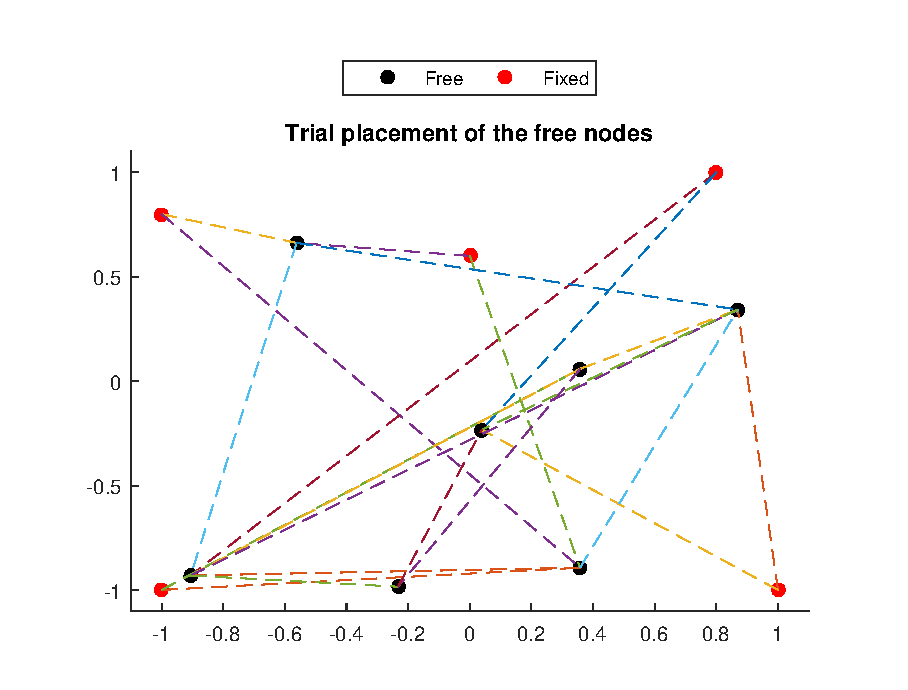
\includegraphics[width=\textwidth]{matrixrand}
\caption{Plot of randomly selected free cells.}
\end{subfigure}
\begin{subfigure}{0.45\textwidth}
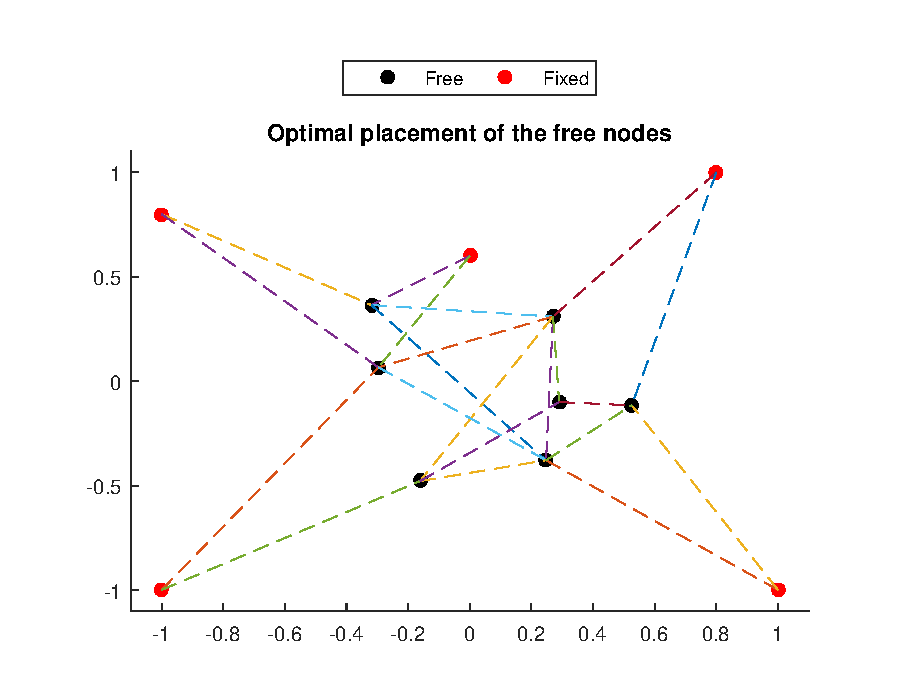
\includegraphics[width=\textwidth]{matrixopt}
\caption{Plot of free cells selected by minimizing \autoref{matrix:AxAy}.}
\end{subfigure}
\caption{Plot of the fixed and free cells incl. their wiring.}
\label{matrix:fig}
\end{figure}

On \autoref{matrix:fig} the fixed and free cells are seen where they're randomly selected or optimized. Since they're connected to each other and/or the fixed cells it makes sense that the optimized cells are closer to the center of the fixed cells than when randomly selected.

\part{Pre-analysis \& requirements}\label{pt:preanalysis_req}
%
\chapter{Introduction}\todo{Should be revised - Mathias}
This project deals with the design of a stabilization system based on modelling of a rocket.
%within the atmosphere of Earth. 

On the 15th of february 2017 an Indian rocket successfully launched with a payload of 104 satellites. The rocket beat the previous payload record for a Russian rocket carrying 37 satellites. This is a accomplishment and important milestone for rockets, but in the early days rocket was not developed based on space travelling.

Rockets is a technology used for hundreds of years. In the 13th century the Chinese and Mongols used fire based rocket, which had chemical mixed gunpowder as propulsion. Trough the 14th and 15th century the gunpowder improved and the rockets range increased, but was at this time considered as weapons.  

The understanding of modern rockets was based on experiments with steam propulsion as with for example the aeolipile in the 17th century. Aeolipile is a rocket-like sphere, that rotates trough directing pressurised steam trough opposite pointing L-shaped nozzles\cite{web:HistoryRocket}. 

This meant that the approach to rockets became more scientific. In the later 17th century Sir Isaac Newton determined his three laws of motions which led to new understanding in rocket science.

Rocket was still considered as weapons at this state and the accuracy was one of the major problems. The understanding and knowledge of aerodynamics was not yet established at this point. And therefore these rockets could not be used to carry a preservable payload, because of their accuracy and stability. 


From the 20th century and forward the use of rockets rapidly progressed and within the last 60 years rocket have been used for travelling and exploring our atmosphere and space. The development of this has been beneficial for humans, with the sending of satellites into orbit around earth and the scientific exploration of space. Today satellites and space travelling has a wide spread use for communication, scientific research and monitoring, which benefits most people on daily basis. This was not possible without the development of stable rockets that is able to carry a payload\cite{web:HistoryRocket}.


The early days problems of rockets was the short travelling distance. Therefore the focus was on having better thrust to gain further distances. The design of liquid fuel motors lead to that distance no longer was a problem. The main concern was the amount of fuel needed and the weight of the payload. The heavier the rocket is the more fuel it needs, and adding more fuel makes the rocket heavier. Incorrect distribution of the fuel could therefore make the rocket unstable, because of the change in the rockets center of gravity.


Stability and inaccuracy was also one of the major concerns in 19th century rockets. The rockets was designed with the thruster placed in the top/front, similar to how fireworks are designed today. This causes instability if the thruster is not powerful enough or the weight distribution is incorrect. As well does a disturbance as wind etc. effect the stability. But as we know from modern full scale rockets the thruster is placed at the bottom, which gives a higher risk of instability problems. When the thrust is applied from the bottom the rocket needs to be stable in the top. If the rocket becomes unbalanced at tip, the more likely it is to deviate from its path. 



\bigbreak
Incorrect weight distribution, faulty design, and aerodynamics is factors that all could lead to instability in rockets. These stability problems has all been faced throughout the history of rocket development, and will therefore be further examined to determine if a electronic control system can be implemented to improve the stability issues of rockets.




%
\chapter{Initial Problem Statement}
In order to design and implement a controller that can ensure a stable launch and flight of a rocket the following questions needs answering: 

\textit{How much is the stabilization of the inverted pendulum similar to the flight control of a rocket in the early stages?}
\bigbreak
\begin{itemize}[noitemsep]
\item Is the model of the inverted pendulum is similar rocket's flight control?
\item Can the inverted pendulum and the rocket be controlled using similar control methods?
\end{itemize}



\graphicspath{{figures/technical/}}

\chapter{Preliminary Analysis of a Rocket}
The following chapter describes the functionality and structure behind a rocket. The goal is to determine which factors that leads to instability in flight and launch of a rocket. 



The full scale rocket model that will be described consist of,
\begin{itemize}[noitemsep]
\item a payload system.
\item a guidance system.
\item a propulsion system. 
\item a structural system.
\end{itemize}    
The model is seen cf. figure \ref{fig:RocketStructure}.
\begin{figure}[htbp]
	\centering
 	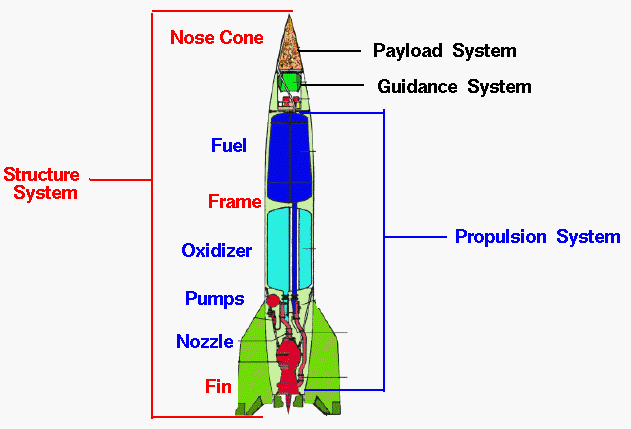
\includegraphics[width=0.65\textwidth]{figures/RocketStructure.png} 
 	\caption{Structure of a full scale rocket\cite{web:RocketStructure}.}
 	\label{fig:RocketStructure}
\end{figure}
%https://spaceflightsystems.grc.nasa.gov/education/rocket/rockpart.html

\textbf{Payload System}\\
Most rockets has some form of a payload system. The goal of the payload system is to carry different objects to its wanted destination. The payload can be everything from satellites and astronauts to fireworks depending on the purpose of the rocket. The payload should be considered when looking at the stability of the rocket, because incorrect weight distribution in the rocket, could lead to aerodynamic and structural instability. 


\textbf{Guidance System}\\
All rockets that has the goal to be directed or controlled includes a guidance system. The guidance system consist of a processors, sensors, radars, and  a form of wireless communication. Its purpose is to control the stability, direction and rotation of the rocket during launch and in flight. The guidance system is developed based on the understanding of forces acting rocket and its motion. The guidance system in moderne rockets often actuate on the propulsion and nozzle system to correct rotation and direction of the rocket.

\textbf{Propulsion System}\\
The propulsion system of a rocket is the part which thrust the rocket. Thrust is the the main force that makes the rocket launch and fly. All propulsion systems is based on Newton's third law. This means that a propulsion system should be able make a combustion which produces a downwards force high enough to launch the structural system of the rocket.


The propulsion system can either be a liquid rocket engine or a solid rocket engine. A liquid rocket engine is based on a combustion of fuel and a oxidizer which is mixed an burned. The resulting gas of the burn, is directed trough a nozzle which accelerates it.
A solid rocket engine has premixed oxidizer and fuel which becomes the propellant. This propellant is compressed into a cylinder with an hole in it that functions as a combustion chamber. Which means that after ignition the propellants surface functions as the combustion chamber. The gas is therefore also forced trough a nozzle that accelerates it. Which applies i force to the engine that gives a launch of the rocket. 


\textbf{Structural System}\\
Close to all full scale rockets consist of a structural system. The system consist of the cylindrical body/frame, a nose cone with the payload system and the fins that ensures a stable aerodynamic profile. Though most newer full scales rocket does not rely only on aerodynamics to ensure stability\cite{web:RocketStructure}.
\bigbreak   

The correct combination of the system modules should ensure a stable flight. \todo{Write something about instability based on the introduction.} 

%All based on https://spaceflightsystems.grc.nasa.gov/education/rocket/rockpart.html

\subsection{Controlling a Rocket's Stability}
The design method for placing the CP and GP does not always provide a perfectly stable attitude control. Indeed to have such precision an active control system is necessary. Full scale rockets use the thrusting force to achieve alike control. In order to do so most of them operate with the gimbaled thrust method. It consists of steering the engine's nozzle to get the thrusting force in right incidence. An example is seen cf. figure \autoref{fig:RocketGimbal}. 
\begin{figure} [htbp]
	\centering
	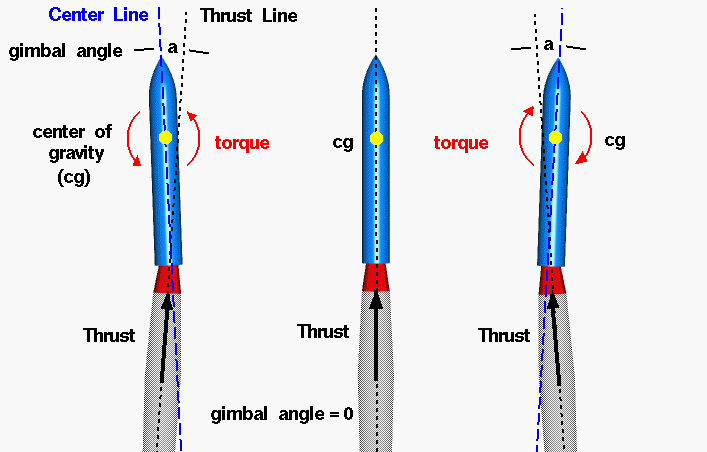
\includegraphics[width=0.8\linewidth]{RocketGimbal}
	\caption{Example of gimballing a rocket nozzle \cite{web:rocketnasa}.}
	\label{fig:RocketGimbal}
\end{figure}
\newpage

Where a torque is applied to create a rotation around the rocket's center of gravity. The thrust direction is relative to the position of the center of gravity.  This should compensate for direction deviations from the rocket's center line or trajectory, and keep the rocket stable. The described gimbal method will be the control method focused on in this project. The rocket will be designed with a control system depending on vectoring the thruster in relation to the attitude position of the rocket. 


\section{Mechanical System of a Rocket}
Input/output relation of a rocket.
\section{Systems with Similar Instability Problems}
\graphicspath{{figures/"Preanalysis&Requirement"/SimilarSystems/}}

In order to stabilize the rocket in flight, a controller must be implemented to correct the rockets trajectory deviation during flight.

The possibility of damaging the rocket or the controller needs to be countered by the efficiency of the control system.


Experimenting such a system during flight is expensive and presents nonnegligible hazards.
Is there a system that has similar instability properties of rockets, and presents fewer restrictions to experiment?

The Cubli is a system known for its instability. It is commonly used in Control Theory to analyze the behavior of a reaction of a wheel inverted system. The advantages of the usage a Cubli is its ability to reach its equilibrium position in microgravity environments, such as asteroids. This is not relevant for a rocket instability project. And can therefore not be directly related to the instability of a rocket.

A recent technology facing instability is Segway. A Segway is an application of an inverted pendulum to a two wheeled self-balance vehicle. The objective is to detect and stabilize the instability of the vertical stick to move the vehicle and prevent the user to fall. This vehicle requires three body directions instead of the linear motion of an inverted pendulum. The study of instability properties of a Segway system would mean the study of elements nonexistent or negligible in a rocket system.

An inverted pendulum objective is to stabilize a stick whose center of mass is above pivot point. The process is done using a horizontal force, resulting in a first degree of freedom rotation, as found in a rocket system. A double inverted pendulum is a combination of an inverted pendulum and a double pendulum. The stability of the stick is reached by applying a torque between the two pendulums. To reach the equilibrium position of a rocket in flight, the aileron must create a torque to counter the lift force.
%\begin{figure}[htbp]
%	\centering
%	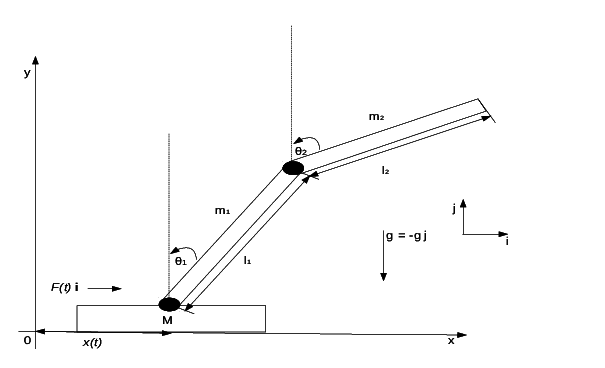
\includegraphics[width=0.6\linewidth]{double-inverted-pendulum}
%	\caption{Summary of forces applied to a double inverted pendulum. The process is equivalent to figure  \vref{fig:RocketForceSummary}.}
%	\label{fig:DoubleInvertedPendulum}
%\end{figure}

In consideration of the different applications and similarities of the three systems, the double inverted pendulum will be further analyzed. The objective is to model the dynamics of both the double inverted pendulum and the rocket, and then compare and relate the models to determine similarities. This should lead to designing a control system for stabilizing the inverted pendulum, which could be implemented on the rocket as a stabilization control system. 




\section{The Inverse Pendulum}
relate the rocket model to a Inverse Pendulum

\chapter{Delimitation}
In the project some limits has to be set for the use of models and materials. The objective of the control system is to find the similarities of using a electronic stabilization system for rockets and for inverted pendulums. The system is developed as a proof-of-concept solution. The models in the project can only be approximations of reality, and it is therefore observable that the transfer to a larger scale project will not be linear.        

\textbf{Physical delimitation:}
The inverted pendulum setup used in the project is pre-fabricated and made available by the university.  The choice of motor, gears, and other components will therefore not be further considered. The setup is a double inverted pendulum, and contains therefore of both a arm and a stick. The double inverted pendulum setup will be from here on be called "inverted pendulum". The setup is shown cf. figure \ref{fig:InvertedPendulum1}.
\todo{Figure should be updated with lengths and gear teeth, block seperating the individual systems.}
\begin{figure}[htbp]
	\centering
	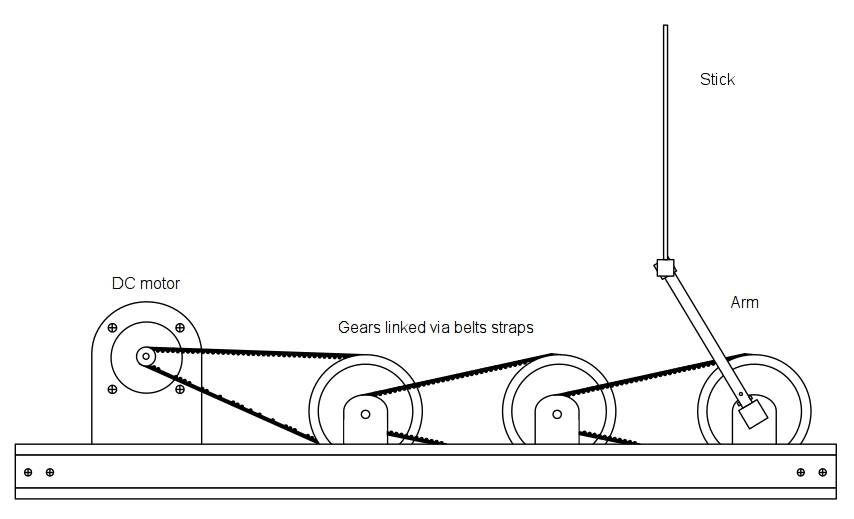
\includegraphics[width=0.7\linewidth]{figures/"Preanalysis&Requirement"/invertedPendulumDiagram}
	\caption{Diagram of the inverted pendulum setup\citep{web:BalancingStick2008}.} \label{fig:InvertedPendulum1}
\end{figure}


Construction and modeling of the rocket will be limited to a minor-scale rocket with a similarities to the design behind a full-scale rocket. The rocket will be designed around a solid propellant thruster, and will therefore not contain any liquid fuel. This is to limit the constraints from laws and keep the cost low. Further more weight and dimension limits is set before designing the rocket.
 
 
\textbf{Control delimitation:}
A choice is made that the starting point for controlling the stick is as illustrated cf. figure \ref{fig:InvertedPendulum1} in upwards vertical position. Therefore the controller will not be able to balance the stick, if its vertical balance limits is surpassed. The delimitation is made to simplify the controlling, and make it as similar as possible to controlling a rocket. 
 
 
\textbf{Test delimitation:}
Launching and flight of a rocket for testing a controller is a high cost procedure because of the chance of damaging the rocket and the cost of thrusters per launch. The testing of the rockets stabilization will be ground based test setup, where the controller can be tested without the risk of damaging the rocket. If, and only if the control system proves stable and safe, a launch and flight of the rocket will be conducted under circumstances fulfilling given laws.   
\bigbreak


The delimitation sets the boundaries for the project and describes which models is available. This gives possibility for describing and modeling of both the inverted pendulum and rocket, to examine if there is similarities behind controlling them. 

\chapter{Inverted pendulum analysis}


\section{Inverted pendulum description}
For this project an inverted pendulum set up is given. It consists of:
\begin{itemize}
	\item a DC motor
	\item a system of four gears linked by belt strap
	\item an arm
	\item a stick connected to the end of the arm with a liberty of movement of one degree
\end{itemize}

\begin{figure} [htbp]
	\centering
	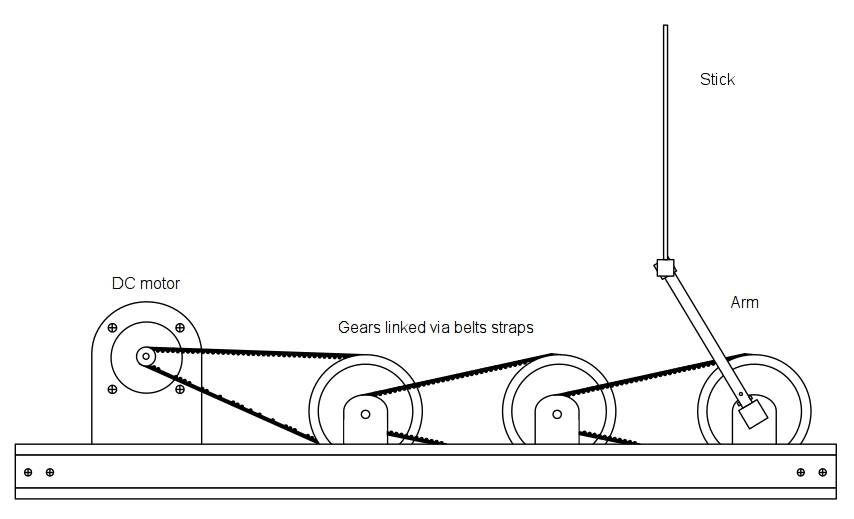
\includegraphics[width=0.8\linewidth]{figures/"Preanalysis&Requirement"/invertedPendulumDiagram}
	\caption{Diagram of the set up fully assembled} \label{fig:InvertedPendulumSetUp}
\end{figure}

\autoref{fig:InvertedPendulumSetUp} is a diagram of the set up when fully assembled. The DC motor moves the arm via the gears, a noteworthy fact is that out the four gears three are of the same size. This means that two gears do not have any influence on the torque and the angular velocity of the arm.

\section{Inverted pendulum modelling}
put the modelling section there

\graphicspath{{figures/modeling/gearTrain/}}
\section{Modeling of the Gear System}\label{sec:ModGearSys}
In this section, the gear system will be modeled. 

\todo [inline,author=Geoff]{Work on intro and maybe put figure}


Three transfer functions are going to be determined in this section. First, the transfer of the motor's angular velocity $\omega_m$ to the angle of the arm $\theta_a$ through the gears. Then, too transfer functions are needed for $\tau_L$: the torque of the load comes from both the torque of the arm and stick $\tau_{as}$ and, considering the frictions in the gears, from $\omega_m$ itself.


\subsection{Relation between $\Omega_m$ and $\Theta_a$}

\begin{figure}[htbp]
	\centering
 	
\includegraphics[width=1\textwidth]{figures/FigureIsComing.PNG} 
 	\caption{Part of the gear structure. The whole gear system consists of three of them.}
 	\label{fig:GearPart}
\end{figure}


From \autoref{fig:GearPart}, considering the small wheel as the one connected to the motor, if the motor shaft turns, the belt joining the small and the big wheel will make them turn the same distance:
\begin{equation}
	\theta_m r_m = \theta_w r_w
\end{equation}

This expression is then differentiated to find the relation with the angular velocities:
\begin{equation}
	\omega_m r_m = \omega_w r_w
	\label{eq:AngularVelRelation}
\end{equation}

The gear ratio is defined as: 
\begin{equation}
	N = \frac{r}{R}
	\label{eq:GearRatio}
\end{equation}

As the gear system is composed by three similar connected wheels structures like shown in \autoref{fig:GearPart}, the ratio between small wheel x, $r_x$, and big wheel x, $R_x$ is the same:
\begin{equation}
	\frac{r_x}{R_x} = \frac{r_{motor}}{R_{w_1}} = \frac{r_{w_1}}{R_{w_2}} = \frac{r_{w_2}}{R_{w_3}} = N
\end{equation}

Knowing this and since $\omega_m$ is transferred through three gears, the relation between the angular velocity of the motor $\omega_m$ and the angle of the arm $\theta_a$ is found following the principle of \autoref{eq:AngularVelRelation}:
\begin{subequations} \label{eq:tech_ToA}
	\begin{flalign}
		&\dot{\theta}_a(t) = N^3 \omega_m(t) \\
		&\dot{\theta}_a(t) = N^3 \int_{0}^{t}\omega_m(v) dv \\
		&\mathcal{L}\{\dot{\theta}_a(t)\} = \Theta_a(s) = N^3 \cdot \frac{1}{s} \Omega_m(s)
	\end{flalign}
\end{subequations}

The transfer function from the motor's angle velocity to the angle of the arm is:
\begin{equation}\label{eq:thetaOmega}
	\frac{\Theta_a(s)}{\Omega_m(s)} =  \frac{N^3}{s}
\end{equation}

\subsection{Linear Model}
\todo[inline,author=Geoff]{Why linear model?}

In order to design an effective feedback control system a linear models is a necessity. As seen previously in \autoref{eq:thetaOmega} $\frac{\Theta_a(s)}{\omega_m(s)}$ is already a linear relationship. So in order to get a linear system only the transfer function $\frac{\omega_m(s)}{U(s)}$ has to be linearized.

It can be seen from \autoref{eq:DCMotorTFWithLoad}, that in order to linearize $\frac{\omega_m(s)}{U(s)}$ $\tau_l$ has to be rewrite in function of $U(s)$ and $\omega_m(s)$.

\subsection{Determining $\tau_l$}
As said in \autoref{sec:ModGearSys} $\tau_l(s)$ is the torque of the load. In the inverted pendulum case the load is composed of the friction and the torque necessary to counter the gravity which result in \autoref{eq:TauL}.

\begin{equation}\label{eq:TauL}
	\tau_l = \tau_{f_{gear}} + \tau_{as}
\end{equation}

It is necessary then to derive $\tau_{f_{gear}}$ and $\tau_{as}$ to see if they are requiring linearization.

\subsubsection*{Determining $\tau_{f_{gear}}$}
The gear train is composed by three identical belt and pulley system. \autoref{fig:Belt&Pulley} corresponds to the first system between the motor and the first wheel. 
\begin{figure}[htbp]
    \centering
    
\includegraphics[width=1\textwidth]{figures/FigureIsComing.PNG}
    \caption{Body diagram of a belt and pulley system}
    \label{fig:Belt&Pulley}
\end{figure}

\startexplain
\explain{$J_m$ is the moment of inertia of the motor}{\si{\kilogram\meter\squared}}
\explain{$J_w$ is the moment of inertia of the wheel}{\si{\kilogram\meter\squared}}
\explain{$\omega_m$ is the motor's angular velocity}{\si{\meter\per\second}}
\explain{$\tau_m$ is the torque of the motor}{\si{\newton\meter}}
\explain{$F_1$ is the force transferred from the motor to the wheel}{\si{\newton}}
\explain{$r$ is the radius of the motor's wheel}{\si{\meter}}
\explain{$R$ is the radius of the wheel}{\si{\meter}}
\explain{$\tau_{f_{gear}}$ is the torque of the gear train friction}{\si{\newton\meter}}
\explain{$\tau_L$ is the torque of the wheel's load}{\si{\newton\meter}}
\explain{$b_w$ is the viscous friction coefficient of the wheel}{\si{\newton\meter\per\radian\per\second}}
\stopexplain



\begin{figure}[htbp]
    \centering
    
\includegraphics[width=1\textwidth]{figures/FigureIsComing.PNG}
    \caption{Body diagram of the motor wheel}
    \label{fig:BodyDiagramsMotorWheel}
\end{figure}

Using the previously stated $2^{nd}$ law of motion, the mechanical equation for the motor wheel can be found from \autoref{fig:BodyDiagramsMotorWheel}:

\begin{equation}
    J_m \dot{\omega}_m = \tau_m + F_1r - b_m\omega_m
    \label{eq:MotorfreeBody}
\end{equation}

For the body diagram for the wheel in \autoref{fig:BodyDiagramsMotorWheel}:
\begin{equation}
	J_w\dot{\omega}_w = -F_1R -\tau_l -b_w\omega_w
\end{equation}

Looking at the whole gear train, $\tau_{f_{gear}}$ represents the total friction and $\tau_L$ is the opposite of the torque transferred to the next wheel. Which gives for wheels 1, 2 and 3:

\begin{subequations} 
	\begin{flalign} \label{eq:GiveMeAnOriginalName}
		&J_{w_1}\dot{\omega}_{w_1} = -F_1R + F_2r -b_{w_1}\omega_{w_1} \\ 
		&J_{w_2}\dot{\omega}_{w_2} = -F_2R + F_3r -b_{w_2}\omega_{w_2} \\ 
		&J_{w_3}\dot{\omega}_{w_3} = -F_3R - b_{w_3}\omega_{w_3} 
	\end{flalign}
\end{subequations}

Using the relation in \autoref{eq:AngularVelRelation}, the angular velocity of each wheels can be found according to $\omega_m$:
\begin{subequations} 
	\begin{flalign}
		&\omega_{w_1} = N \omega_m \\
		&\omega_{w_2} = N \omega_{w_1} = N^2 \omega_m \\
		&\omega_{w_3} = N \omega_{w_2} = N^3 \omega_m
	\end{flalign}
\end{subequations}

The same equations are valid with angular accelerations.
Which gives for Equations \ref{eq:GiveMeAnOriginalName}:
\begin{subequations} 
	\begin{flalign}  
		&J_{w_1}N\dot{\omega}_m = -F_1R + F_2r -b_{w_1}N\omega_m \\ 
		&J_{w_2}N^2\dot{\omega}_m = -F_2R + F_3r -b_{w_2}N^2\omega_m  \\ 
		&J_{w_3}N^3\dot{\omega}_m = -F_3R - b_{w_3}N^3\omega_m 
	\end{flalign}
\end{subequations}

The total friction torque $\tau_{f_{gear}}$ in the gear train is the torque that needs to be overcome by the torque of the motor in order to make the gear train move. It means that when the gear train is static:

\begin{subequations} \label{eq:findTauf}
	\begin{flalign}
		&\omega_m = 0\\
		&\tau_m \leqslant \tau_{f_{gear}}
	\end{flalign}
\end{subequations}

To find $\tau_{f_{gear}}$, the special case where $\tau_m = \tau_{f_{gear}}$ is studied. Inserting \autoref{eq:findTauf} into \autoref{eq:MotorfreeBody}:

\begin{equation} 
		\tau_{f_{gear}} = -F_1 \cdot r
		\label{eq:TaufF1r}
\end{equation}

$F_1$ needs to be isolated from \autoref{eq:GiveMeAnOriginalName}. Each forces $F_1$, $F_2$ and $F_3$ are then isolated, giving: 

\begin{subequations} 
	\begin{flalign}
		&F_1 = -\frac{1}{R} (b_{w_1}N\omega_m + J_{w_1}N\dot{\omega}_m - F_2r) 	\label{eq:F1}\\ 
		&F_2 = -\frac{1}{R} (b_{w_2}N^2\omega_m +  J_{w_2}N^2\dot{\omega}_m - F_3r)	\label{eq:F2}\\
		&F_3 = -\frac{1}{R} (b_{w_3}N^3\omega_m + J_{w_3}N^3\dot{\omega}_m)			\label{eq:F3}
	\end{flalign}
\end{subequations}

Inserting \autoref{eq:F3} in \autoref{eq:F2}, then \autoref{eq:F2} in \autoref{eq:F1}, the expression of $F_1$ according to the friction and moment of inertia of each wheel is found:

\begin{flalign}
	F_1 = &-\frac{1}{R} N(b_{w_1}\omega_m + J_{w_1}\dot{\omega}_m \notag \\
	& +\frac{r}{R} N^2(b_{w_2}\omega_m + J_{w_2}\dot{\omega}_m \notag \\
	& +\frac{r}{R} N^3(b_{w_3}\omega_m + J_{w_3}\dot{\omega}_m)))
\end{flalign}


Using \autoref{eq:TaufF1r} and the gear ratio in \autoref{eq:GearRatio}, the total friction is given by: 
\begin{align} \label{eq:TaufTimeDomain}
	\tau_{f_{gear}} =&\ N^2 (b_{w_1}\omega_m + J_{w_1}\dot{\omega}_m \notag \\
	& +N^3 (b_{w_2}\omega_m + J_{w_2}\dot{\omega}_m \notag \\
	& +N^4 (b_{w_3}\omega_m + J_{w_3}\dot{\omega}_m)))
\end{align}


\autoref{eq:TaufTimeDomain} is Laplace-transformed:

\begin{flalign} \label{eq:TaufLaplaceDomain}
	\mathcal{L}\{\tau_{f_{gear}}(t)\} = \tau_{f_{gear}}(s) = &\ N^2 (B_{w_1}\Omega_m + sJ_{w_1}\Omega_m \notag \\
	& +N^3 (B_{w_2}\Omega_m + sJ_{w_2}\Omega_m \notag \\
	& +N^4 (B_{w_3}\Omega_m + sJ_{w_3}\Omega_m)))
\end{flalign}


\autoref{eq:TaufLaplaceDomain} is reorganized to find the final expression for $\tau_{f_{gear}}$ in \autoref{eq:TaufReorganized}:
\begin{equation}
	\tau_{f_{gear}} = \left[(N^2 J_1 + N^3 J_2 + N^4 J_3)s +( N^2 B_1 + N^3 B_2 + N^4 B_3)\right]\Omega_m
	\label{eq:TaufReorganized}
\end{equation}











\subsubsection*{Determining $\tau_{as}$}
\todo [inline,author=Geoff \& Maxime]{The different tau need to be better introduced and their relation needs to be clarified with an equation in the beginning of this section}
$\tau_{as}$ is the torque necessary for the arm to counter the load applied by the arm and the stick. It can be divided into two parts.

The first part, $\tau_a$, is the torque generated by the arm.

 This torque is generated when the arm is not parallel to the gravitational force. As seen in \autoref{fig:tauA} this force can be seen as a pendulum where the mass is concentrated in the GC and has a weightless rod, so the gravitational force can be summarized as \autoref{eq:tauA}.

\begin{figure}[htbp]
	\missingfigure{A diagram showing how the gravity affects the arm}
	\caption{Diagram of the gravitational force on the arm}\label{fig:tauA}
\end{figure}

\begin{equation}\label{eq:tauA}
	\tau_a=M_a\cdot g \cdot \frac{l_a}{2} sin(\Theta_a) \addunit{\newton\meter}
\end{equation}
\startexplain
\explain{$M_a$ is the mass of the arm}{\si{\kilogram}}
\stopexplain

Another torque $\tau_{am}$ is also generated by the momentum of the arm when it moves. This can be translated by the \autoref{eq:ArmMomentum}.

\begin{equation}\label{eq:ArmMomentum}
	\tau_{am}=\dot\omega_a\ \cdot J_a \addunit{\newton\meter}
\end{equation}
\startexplain
\explain{$\omega_a$ is the angular velocity of the arm}{\si{\meter\per\second}}
\explain{$J_a$ is the moment of inertia of the arm}{\si{\kilogram\meter\squared}}
\stopexplain

The second part, $\tau_s$, is the torque generated by the stick due to the gravity.

Since the stick is connected to one of the extremities of the arm and the load of the arm is already accounted, it is once again a classical pendulum case with weightless rod which can be translated to \autoref{eq:StickGravLoad}.

\begin{equation}\label{eq:StickGravLoad}
	\tau_s = l_a\cdot sin(\Theta_a) \cdot \frac{l_s}{2}\cdot M_s\cdot g\cdot cos(\Theta_s) \addunit{\newton\meter}
\end{equation}

$\tau_{sm}$ is the load generated by the momentum of the stick. According to Newton third law the torque applied on the arm by the momentum will be the opposite of the torque generated by the momentum of the stick. This can be transcribe as \autoref{eq:TauSm}.

\begin{equation}\label{eq:TauSm}
	\tau_{sm}=-J_s\cdot \Theta_s
\end{equation}

\autoref{eq:TauSm} can be then rewritten as \autoref{eq:TauSmLin} as explained in \autoref{sec:StickArm}.

By combining and linearizing Equations (\ref{eq:tauA}), (\ref{eq:ArmMomentum}) and (\ref{eq:StickGravLoad}), \autoref{eq:finalTauL} is obtained.

\begin{flalign}\label{eq:finalTauL}
	\tau_{as} = \ &M_a g  \frac{l_a}{2} \Theta_a+\dot\omega_a\  J_a \notag \\
	&+\frac{l_s}{2}M_s\left(-l_a\dot{\omega}_a+g\theta_s\right)-b_{as}(\omega_s-\omega_a)\notag \\
	&+l_a \Theta_a  \frac{l_s}{2} M_s g \addunit{\newton\meter}
\end{flalign}

Since the system has to correct $\Theta_s$ by moving the arm so that $\omega_s=-\omega_a$, it gives \autoref{eq:FinalTauAS}.

\begin{subequations}\label{eq:FinalTauAS}
	\begin{flalign}
		\tau_{as} =	\ &M_a g  \frac{l_a}{2} \Theta_a+\dot\omega_a\  J_a \notag \\
					&+\frac{l_s}{2}M_s\left(-l_a\dot{\omega}_a+g\theta_a\right)+2\omega_a b_{as}\notag \\
					&+l_a \Theta_a  \frac{l_s}{2} M_s g \addunit{\newton\meter}\\
					\notag \\ 
		\mathcal{L}\{\tau_{as}\} = 	&M_a g  \frac{l_a}{2} \frac{\Omega_a}{s}+\Omega_a s J_a \notag \\
									&+\frac{l_s}{2}M_s\left(-l_a\Omega_a s+g\frac{\Omega_a}{s}\right)-2\Omega_a b_{as}\notag \\
									&+l_a \frac{\Omega_a}{s}  \frac{l_s}{2} M_s g \addunit{1}
	\end{flalign}
\end{subequations} 

\todo [inline,author=Geoff]{This part needs to be moved up}
Since it is a change in the small angles the linearization of a cosine and a sine function gives \autoref{eq:BasLin}.

\begin{subequations}\label{eq:BasLin}
	\begin{flalign}
		&sin(x)=>x \addunit{1}\\
		&cos(x)=>1 \addunit{1}
	\end{flalign}
\end{subequations}

\autoref{fig:BasLinPlot} shows that within an angle variation of \SI{10}{\degree} the approximation of the linearization is acceptable.

\begin{figure}[htbp]
	\centering
	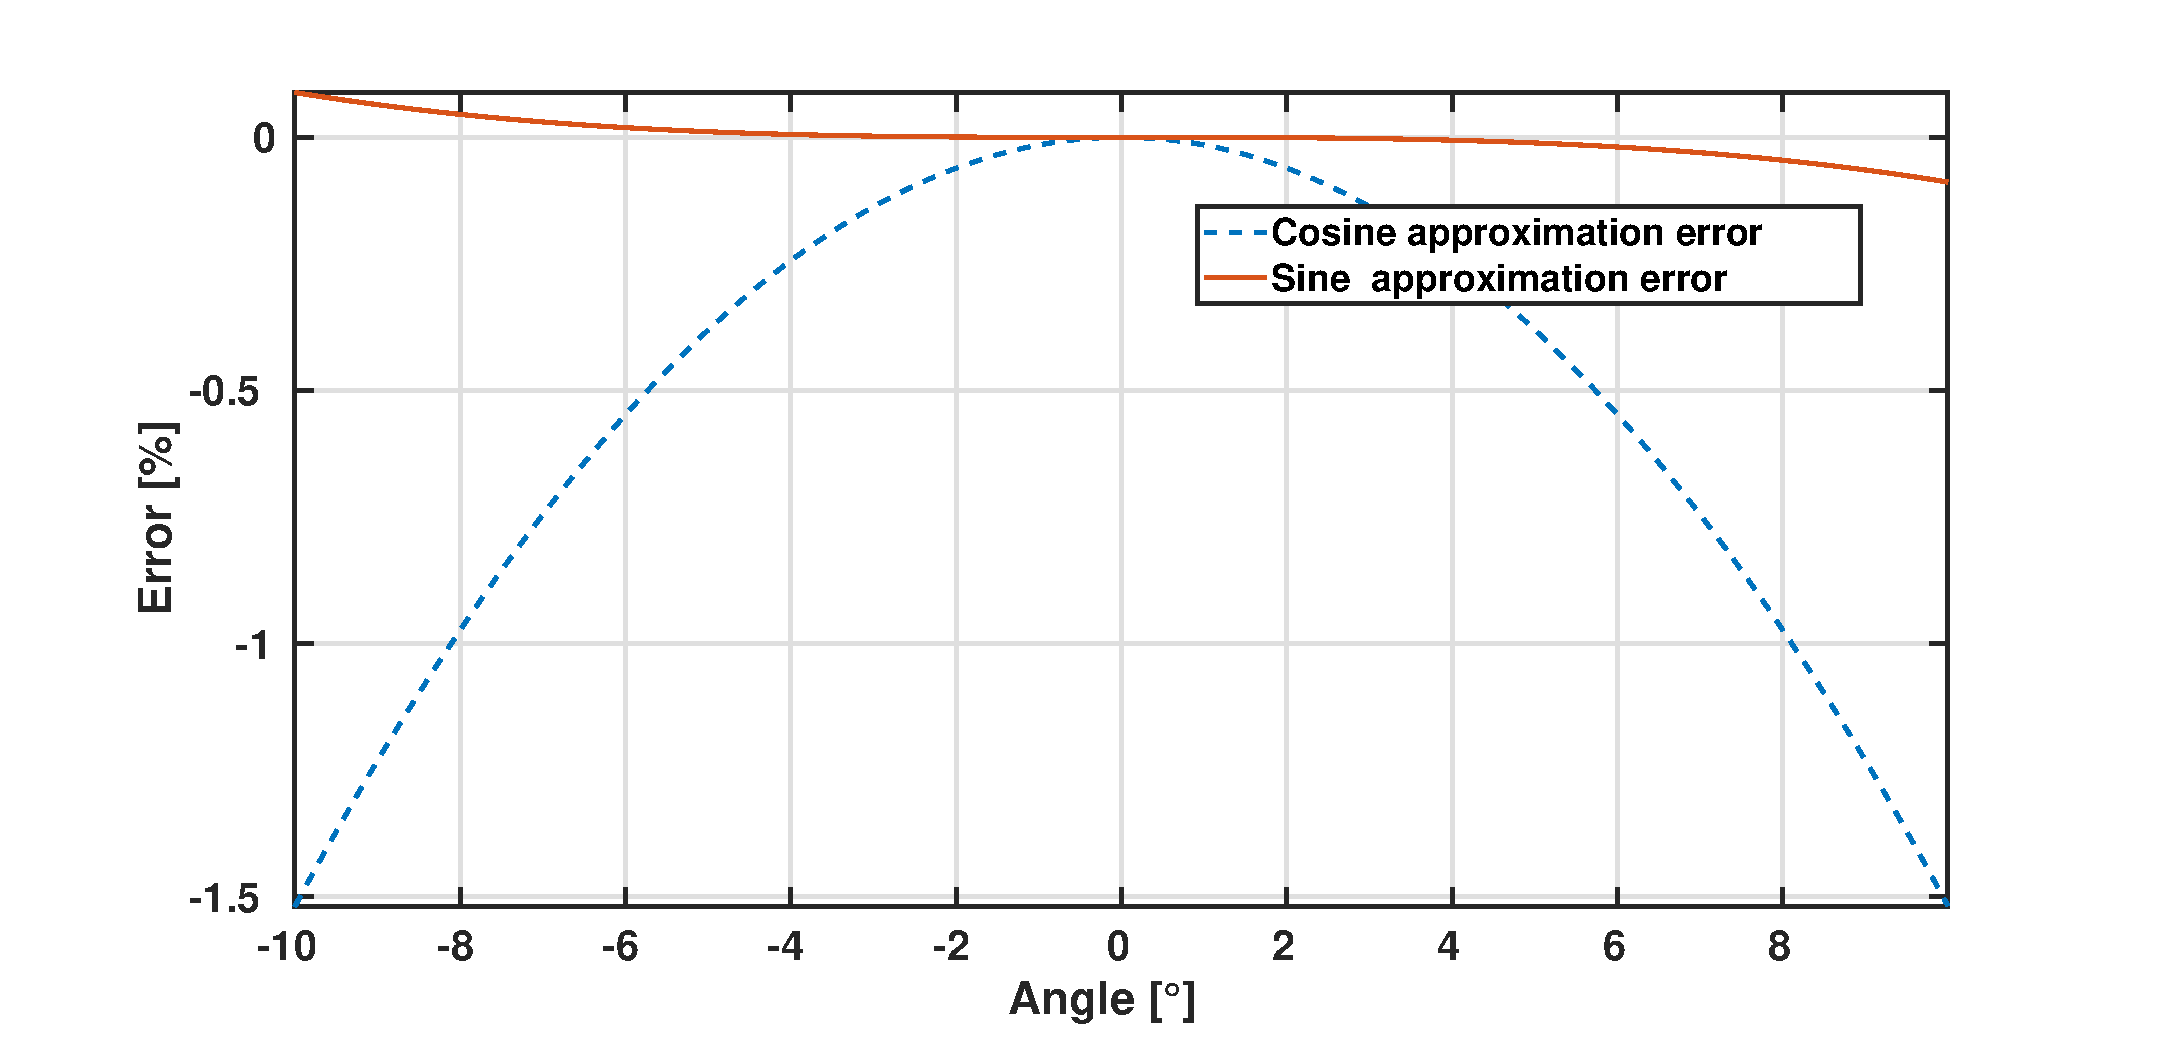
\includegraphics[width=0.8\textwidth]{CosSinLinApprox}
	\caption{Error generated by the approximation of the cosine and the sine function}\label{fig:BasLinPlot}
\end{figure}

\section{Modeling of the DC-Motor}

The purpose of this section is to establish a dynamic model of the DC-motor. This model will result in a transfer function from a voltage input, \textit{Um}, to an angular velocity output, \textit{$\omega_m$}. It will be done by modeling the electrical and the mechanical part of the motor and then putting them together to find the transfer function of the motor.

\subsection*{Electrical Model of the Motor}
The electrical circuit of the motor is presented in \autoref{fig:MotorCircuit}.

\begin{figure}[htbp]
	\centering
 	
\includegraphics[width=1\textwidth]{figures/FigureIsComing.PNG} 
 	\caption{Electric circuit of a DC-motor}
 	\label{fig:MotorCircuit}
\end{figure}

Using Kirchhoff's voltage law, the electric model of the DC-motor is found:
\begin{subequations} \label{eq:tech_ToA}
	\begin{flalign}
		&U_m = R_m \cdot i + L_m \frac{di}{dt} + e \addunit{\volt} \\
		&e = K_e \cdot \omega_m \addunit{\volt}
	\end{flalign}
\end{subequations}

\startexplain
	\explain{$U_m$ is the voltage output of the generator}{\si{\volt}}
	\explain{$R_m$ is the resistance of the DC-motor}{\si{\ohm}}
	\explain{$L_m$ is the inductance of the DC-motor}{\si{\henry}}
	\explain{$i$ is the current in the DC-motor}{\si{\ampere}}
	\explain{$e$ is the electromotive force}{\si{\volt}}
	\explain{$K_e$ is the motor velocity constant}{\si{\volt\second\per\radian}}
	\explain{$\omega_m$ is the angular velocity of the motor}{\si{\radian\per\second}}
\stopexplain

\subsection*{Mechanical Model of the Motor}
The mechanical circuit of the motor is presented in \autoref{fig:MotorBodyDiagram}.

\begin{figure}[htbp]
	\centering
 	
\includegraphics[width=1\textwidth]{figures/FigureIsComing.PNG} 
 	\caption{Body diagram of a DC-motor}
 	\label{fig:MotorBodyDiagram}
\end{figure}

When applied to a rotational movement, Newton's second law of motion state that the sum of the torques applied to an object equals the moment of inertia times the angular acceleration of this object. From \autoref{fig:MotorBodyDiagram}, the equation for the mechanical part of the motor is found:

\begin{equation}
	J_{m} \dot{\omega}_{m} = \tau_{m} - \tau_{l} - \tau_{fm} \addunit{\newton\meter}
	\label{eq:MotorMechanical}
\end{equation}

\startexplain
	\explain{$J_m$ is the moment of inertia of the motor}{\si{\kilo\gram\meter\squared}}
	\explain{$\omega_m$ is the angular velocity of the DC-motor}{\si{\radian\per\second}}
	\explain{$\tau_m$ is the torque of the DC-motor}{\si{\newton\meter}}
	\explain{$\tau_l$ is the torque of the load}{\si{\newton\meter}}
	\explain{$\tau_{fm}$ is the torque of the friction}{\si{\newton\meter}}
\stopexplain

The motor's torque and the friction's torque, respectively $\tau_m$ and $\tau_f$, are defined as:

\begin{subequations}\label{eq:tauLm}
	\begin{flalign}
		&\tau_m = K_t \cdot i \addunit{\newton\meter} \label{eq:MotorTorque}\\	
		&\tau_{fm} = b_{m}\cdot\omega_{m} \addunit{\newton\meter}	\label{eq:FrictionTorque}
	\end{flalign}
\end{subequations}

\startexplain
	\explain{$K_t$ is the motor torque constant}{\si{\newton\meter\per\ampere}}
	\explain{$b_m$ is the viscous friction coefficient}{\si{\newton\meter\second\per\radian}}
\stopexplain

Inserting \autoref{eq:tauLm} into \autoref{eq:MotorMechanical}:
\begin{equation}
	J_{m} \cdot \dot{\omega}_{m} = K_{t} \cdot i - \tau_{l} - b_{m} \cdot \omega_{m} \addunit{\newton\meter}
\end{equation}

\subsection*{Mechanical Model of the Motor}
First, both the electrical and the mechanical equations of the motor need to be Laplace-transformed:
\begin{subequations}
	\begin{flalign}
		&U_{m}(s) = R_{m} \cdot I(s) + s \cdot L_{m} \cdot I(s) + K_{e} \cdot \Omega_{m}(s) \addunit{1} \label{eq:ElectricalLaplace}\\	
		&s\cdot J_{m} \cdot \Omega_{m}(s) = K_{t} \cdot I(s) - \tau_{l} - B_{m} \cdot \Omega_{m}(s) \addunit{1}	\label{eq:MechanicalLaplace}
	\end{flalign}
\end{subequations}

The current, I(s), is isolated in \autoref{eq:ElectricalLaplace}:
\begin{equation}
	I(s)=\frac{U_m(s)-K_e\cdot\Omega(s)}{R_m+sL_m} \addunit{1}
	\label{eq:MotorCurrent}
\end{equation}

Then \autoref{eq:MotorCurrent} is inserted in \autoref{eq:MechanicalLaplace}:
\begin{equation}
	s\cdot J_{m} \cdot \Omega_{m}(s) = K_{t} \frac{U_m(s)-K_e\cdot\Omega(s)}{R_m+sL_m} - \tau_{l} - B_{m} \cdot \Omega_{m}(s) \addunit{1}
	\label{eq:Iinserted}	
\end{equation}

\autoref{eq:Iinserted} is simplified to find an expression for $\Omega_m$: 

\begin{subequations}
	\begin{flalign}
		&\Omega_m(s) \left(sJ_m + \frac{K_tK_e}{R_m + sL_m} + B_m \right) = \frac{K_tU_m(s) - \tau_l(R_m + sL_m)}{R_m + sL_m} \\	
		&\Omega_m(s) = \frac{K_tU_m(s) - \tau_l(R_m + sL_m)}{R_m + sL_m} \cdot \frac{R_m + sL_m}{sJ_m(R_m + sL_m) + B_m(R_m + sL_m) + K_tK_e} \\
		&\Omega_m(s) = \frac{K_tU_m(s) - \tau_l(R_m + sL_m)}{(J_mL_m)s^2 + (J_mR_m + B_mL_m)s + B_mR_m + K_tK_e} \addunit{1} \label{eq:DCMotorTFWithLoad}
	\end{flalign}
\end{subequations}
\autoref{eq:DCMotorTFWithLoad} is the transfer function of the DC-motor from a voltage $U_m(s)$ to an angular velocity $\omega_m$. This equation will be used for the rest of the modeling. 

\todo [inline, author=Geoff]{To be added in the DC-Motor Test appendix when it's created}
For the test of the DC-motor, there is no load. The torque of the load becomes zero, thus changing the expression of $\omega_m$: 
\begin{equation}
	\Omega_m(s) = \frac{K_tU_m(s)}{(J_mL_m)s^2 + (J_mR_m + B_mL_m)s + B_mR_m + K_tK_e} \addunit{1}
\end{equation}











\newpage
\section{Combining the Models for the Inverted Pendulum}\label{sec:CombinedModel}
With a model for each individual part of the inverted pendulum derived, a combined model for the entire system can be made. This model will have voltage, $U_m(s)$, as input and the angle of the stick, $\Theta_s(s)$, as the output. This is done by multiplying all transfer functions together as seen in \autoref{eq:CombTF}.
\begin{flalign}
\frac{\Omega_m(s)}{U_m(s)}\cdot \frac{\Theta_a(s)}{\Omega_m(s)}\cdot \frac{\Theta_s(s)}{\Theta_a(s)}=\frac{\Theta_s(s)}{U_m(s)} \label{eq:CombTF}
\end{flalign}
In block form this is simply done by putting each model sequentially after each other as shown in \autoref{fig:CombBlock}.
\begin{figure}[htbp]
\centering
\missingfigure{Block diagram of the model for the inverted pendulum.}
\label{fig:CombBlock}
\end{figure}

By combining \autoref{eq:Omega_m}, \autoref{eq:thetaOmega} and \autoref{eq:tfArmStick} the model for the inverted pendulum becomes \autoref{eq:CombModel}.
\begin{flalign}
\frac{\Theta_s(s)}{U_m(s)}=\frac{2 K_t s}{A s^3+B s^2 + C s + D}\cdot \frac{N^3}{s} \cdot \frac{-\frac{3l_a}{2l_s}s^2+\frac{3b_{as}}{M_sl_s^2}s}{s^2+\frac{3b_{as}}{M_sl_s^2}s-\frac{3g}{2l_s}} \label{eq:CombModel}
\end{flalign}

 The values for each variable for the inverted pendulum is shown in \autoref{tab:IPModelVar}. The friction between the arm and the stick is assumed to be zero as the joint consists of a ball bearing. The other variables are found in \autoref{sec:IPDesc}, \autoref{} and \autoref{}.
\begin{table}[htbp]
\centering
\caption{Parameters for the inverted pendulum.}
\label{tab:IPModelVar}
\begin{tabular}{llll}
\hline
Variable & Value & Parameter & Unit \\ \hline
$K_t$ & 0.0293 & Mechanical motor constant & \si{\newton\meter\per\ampere} \\
$K_e$ & 0.0355 & Electrical motor constant & \si{\volt\per(\radian\per\second)} \\
$J_m$ & $2.9\cdot 10^{-5}$ & Moment of inertia of the motor & \si{\kilogram\square\meter} \\
$J_{gear}$ & $0.153\cdot 10^{-3}$ & Moment of inertia of the gear & \si{\kilogram\square\meter} \\
$J_a$ & $10.3\cdot 10^{-3}$ & Moment of inertia of the arm & \si{\kilogram\square\meter} \\
$J_s$ & $1.95\cdot 10^{-3}$ & Moment of inertia of the stick & \si{\kilogram\square\meter} \\
$L_m$ & $11.2\cdot 10^{-3}$ & Inductance & \si{\henry} \\
$R_m$ & 1.02 & Resistance & \si{\ohm} \\
$B_m$ & $1.59\cdot 10^{-4}$ & Friction in motor & \si{\newton\per(\radian\per\second)} \\
$B_{gear}$ & $1.11\cdot 10^{-3}$ & Friction in motor & \si{\newton\per(\radian\per\second)} \\
$N$   & 0.3 & Gear ratio & [1] \\   
$l_a$ & 0.33 & Length of arm & \si{\meter} \\
$l_s$ & 0.4 & Length of stick & \si{\meter} \\
$M_s$ & 0.17 & Mass of stick & \si{\kilogram} \\
$b_{as}$ & 0 & Friction between arm and stick & \si{\newton\per(\radian\per\second)} \\  
$g$ & 9.8 & Standard gravitational acceleration & \si{\meter\per\square\second} 
\end{tabular}
\end{table}
\todo[inline,author=maxime]{Ja,Js,Bgear has to be found or a reference to the previous report should be done}
Inserting the numbers from \autoref{tab:IPModelVar} the transfer function of the model for the inverted pendulum becomes \autoref{eq:CombFinalTF}.
\begin{flalign}\label{eq:CombFinalTF}
\frac{\Theta_s(s)}{U_m(s)}=
\end{flalign}

With the mathematical model of the inverted pendulum found a controller for the system can be designed.

\chapter{Rocket Analysis}
		A rocket presents a large number of similarities with an inverted pendulum in terms of modeling and control as it will be demonstrated in this chapter. It also adds one degree of freedom compared to the inverted pendulum.
		For the purpose of studying the problem of rocket control, a model rocket was designed and built. Since mechanical design is out of this work's scope, the engineering of this rocket will not be explained, but the CAD files will be available on the GitHub repository.
		
		
		\section{Rocket Description}
			In this section the rocket model will be described to prepare it's modeling.
			This design consists of 2 sections, that will be called here "stages".
			\begin{itemize}
				\item First stage: propulsion
				\begin{itemize}
					\item {A thruster / Solid Rocket Booster (SRB)}
					\item {A thrust vectoring mechanism, also known as gimbal, with two degrees of freedom}
					\item {Two servo motors for actuating the gimbal}
				\end{itemize}
				\item Interstage:
				\begin{itemize}
					\item {An empty fairing separating the propulsion stage from the electronics}
				\end{itemize}
				\item Upper stage: control
				\begin{itemize}
					\item {A frame to hold the electronics}
					\item {A PCB with a micro-controller}
					\item {A plastic separator with anti-vibration bearings}
					\item {On this separator is placed a gyroscope: the attitude sensor}
					\item A nose fairing
				\end{itemize}
			\end{itemize}
			
			
%				\section{Inverted pendulum and rocket}
%			The goal of this section is to demonstrate the similarities between the inverted pendulum and the rocket stabilization processes, and to define a mathematical model and control loop of the behavior of the angle of the rocket body and the angle of the thruster.
%			
%			The purpose of the system is to guarantee a stable flight to the rocket.
%			The modeling of the flight of a rocket can be divided into two equations: velocity and rotation. In this project, the desired trajectory of the rocket flight is considered to be on the zenith axis. This results in a vertical flight, with then a velocity on the same axis as the trajectory.The rocket's rotation is a circular motion on the bottom-to-nose axis. This create a centripetal force.
%			
%			The displacement angle (gimbal angle) is the difference between the actual flight direction, or bottom-to-nose axis, and the zenith axis. Gimbaled thrust are controllable thrusters used to create a torque and reduce the gimbal angle. 
%			
%			In an inverted pendulum, the objective is to keep the stick in horizontal position. The angle difference between the horizontal and the actual axis of the stick is measured in order to then create a compensation torque with the arm. The arm has the same task as the gimbaled thruster, and the horizontal axis is equivalent to the zenith axis.
%			
%			At the desired initial position of the inverted pendulum, the acceleration of the arm is negligible. This implies that the arm only produces a force on the axis going through the center of gravity of the arm and parallel to the lenght of the arm. This is equivalent to the rocket process where the thruster applies a force on the axis going through the center of gravity of the arm and parallel to the lenght of the thruster. 
%			
%			 Sketch of rocket + IP at initial position
%			
%			Therefore the rocket and the inverted pendulum processes are equivalent for a small displacement angle range. The inverted pendulum is then studied in this project as a first approach to the understanding of rocket in-flight stabilization process.
%			
%			The control loop of the rocket system is described in figure ...
%			
%			Figure of closed loop model of rocket
%			
%			The input of the closed loop is the gimbal angle (angle difference between actual flight direction and zenith axis). The output is the new gimbal angle. In the inverted pendulum, the input and output are also the angle differences, between the horizontal and the actual axis of the stick. 
%			
%			By admiting that the inverted pendulum and the rocket processes are similar the equations found in Section 5.2 Modelling of the Arm and Stick can be applied to the rocket, with the rocket body as the stick and the gimbaled thruster as the arm. However the gravity center of the rocket body is not located in its center. Therefore $l_{a}$ and $\frac{l_{s}}{2}$ become respectively $l_{t}$, for the thruster, and $l_{bg}$, for the lenght from the bottom of the rocket body to its center of mass. The equations describing the forces, with $a$ for arm and $s$ for stick respectively replaced by $t$ for thruster and $b$ for rocket body, are:
%			
%			Transfer function as in part "modeling of stick".
		
		\section{Modeling of the rocket body and stick}
			
		The purpose of this section is to have a mathematical model for the different forces applied on the rocket in flight. 
		
		In this project, the trajectory of the rocket is on the zenith axis, or y axis. Moreover the rocket movement will be at low speed. This implies the impact of the lift on the rocket is negligible. The sum of the forces applied on a rocket in flight can then be described by equation \vref{eq:F_total}:
		
		\begin{equation}
		F_{total} = m*a = F_{thrust} + F_{drag} - F_{gravity} \addunit{\newton} \label{eq:F_{total}}
		\end{equation}
		\startexplain
		\explain{$F_{total}$ is the sum of all force}{\si{\newton}}
		\explain{$F_{thrust}$ is the force created by the gimbaled thruster}{\si{\newton}}
		\explain{$F_{drag}$ is the drag force on the rocket}{\si{\newton}}
		\explain{$F_{gravity}$ is the gravity applied on the rocket}{\si{\newton}}
		\stopexplain
		
		The drag force can be expressed by equation \vref{eq:F_drag}:
		\begin{equation}
		F_{drag} = \frac{1}{2} \cdot C_{d} \cdot \rho \cdot A \cdot v^2 \si{\newton} \label{eq:F_{drag}}
		\end{equation}
		\startexplain
		\explain{$C_{d}$ is the coefficient of drag}{\si{1}}
		\explain{$\rho$ is the air density}{\si{\kilo\gram\per\meter\cubed}}
		\explain{$A$ is the cross sectionnal area of the rocket}{\si{\meter\squared}}
		\explain{$v$ is the velocity of the rocket}{\si{\meter\per\second}}
		\stopexplain
			
		The coefficient of drag and the cross sectionnal area vary depending on the shape of the rocket. Altitude and humidity in the air can impact the air density. Parasit drag can appear due to the surface material or pressure drag.
		
		The gravity force equation is \vref{eq:F_{gravity}}:
		\begin{equation}
		F_{gravity} = m \cdot g \addunit{\newton} \label{eq:F_{gravity}}
		\end{equation}
		\startexplain
		\explain{$m$ is the mass of the rocket}{\si{\kilo\gram}}
		\explain{$g$ is the gravitational acceleration}{\si{\meter\per\second\squared}}
		\stopexplain
			
		
		The thrust force is \vref{eq:F_{thrust}}:
		\begin{equation}
		F_{thrust} = v_{e} \cdot \ddot{m} + A (P_{e} -P_{0}) \addunit{\newton} \label{eq:F_{thrust}}
		\end{equation}
		\startexplain
		\explain{$v_{e}$ is the velocity of the gimbaled thruster}{\si{\meter\per\second}}
		\explain{$\ddot{m}$ is the mass flow rate}{\si{\kilo\gram\per\second}}
		\explain{$A$ is the nozzle exit area}{\si{\meter\squared}}
		\explain{$P_{e}$ is the pressure of the nozzle exit}{\si{\kilo\gram\per\meter\per\second\squared}}
		\explain{$P_{0}$ is the free stream pressure}{\si{\kilo\gram\per\meter\per\second\squared}}
		\stopexplain
		
		
		The thruster pression and velocity is divided into two equation, respectively ahead and behind the propeller nozzle: $P_{o}$ \vref{eq:P_{o}} and $P_{e}$ \vref{eq:P_{e}}.
		
		\begin{equation}
		P_{0} = p_{0} + 0.5 \cdot \rho \cdot(v_{o})^2 \addunit{\kilo\gram\per\meter\per\second\squared} \label{eq:P_{o}}
		\end{equation}
		\startexplain
		\explain{$p_{o}$ is the static pressure}{\si{\kilo\gram\per\meter\per\second\squared}}
		\explain{$v_{o}$ is the velocity of the rocket}{\si{\meter\per\second}}
		\stopexplain
		
		\begin{equation}
		P_{e} = p_{o} + 0.5 \cdot \rho \cdot(v_{e})^2 \si{\kilo\gram\per\meter\per\second\squared} \label{eq:P_{e}}
		\end{equation}
		\startexplain
		\explain{$v_{e}$ is the exit velocity of the gimbaled thruster}{\si{\meter\per\second}}
		\stopexplain
		
		Therefore, there is three different cases of truster pression:
		\begin{equation}
		P_{e} = P_{a} \notag
		& P_{e} > P_{a} \notag
		& P_{e} < P_{a} \notag
		\end{equation}
		 insert sketch of the different cases
		 
		 \section{linearisation}
		
		\startexplain
		\explain{$F_x$ is the force in the x direction}{\si{\newton}}
		\explain{$F_y$ is the force in the y direction}{\si{\newton}}
		\explain{$x_b$ is the position of the center of gravity of the rocket in the x direction}{\si{\meter}}
		\explain{$y_b$ is the position of the center of gravity of the rocket in the y direction}{\si{\meter}}
		\explain{$l_t$ is the length of the thruster}{\si{\meter}}
		\explain{$C_g$ is the length between the gimbal and the center of gravity of the rocket}{\si{\meter}}
		\explain{$\theta_t$ is the angle from the thruster to the y-axis}{\si{\radian}}
		\explain{$\theta_b$ is the angle from the rocket body to the y-axis}{\si{\radian}}
		\stopexplain
		All forces, constants and variables that relates to the thruster and rocket body are denoted by a subscripted $t$ and $b$ respectively. 
		
		The behaviour of the rocket can be fully described by three movements; two translatory and one rotary. It can move in the x and y direction and rotate around it's own axis.
		
		%To find the relation between the angles, the free body diagram of the joint of the arm and stick is made on \autoref{fig:freebodystick}.
		%\begin{figure}[htbp]
		%\centering
		%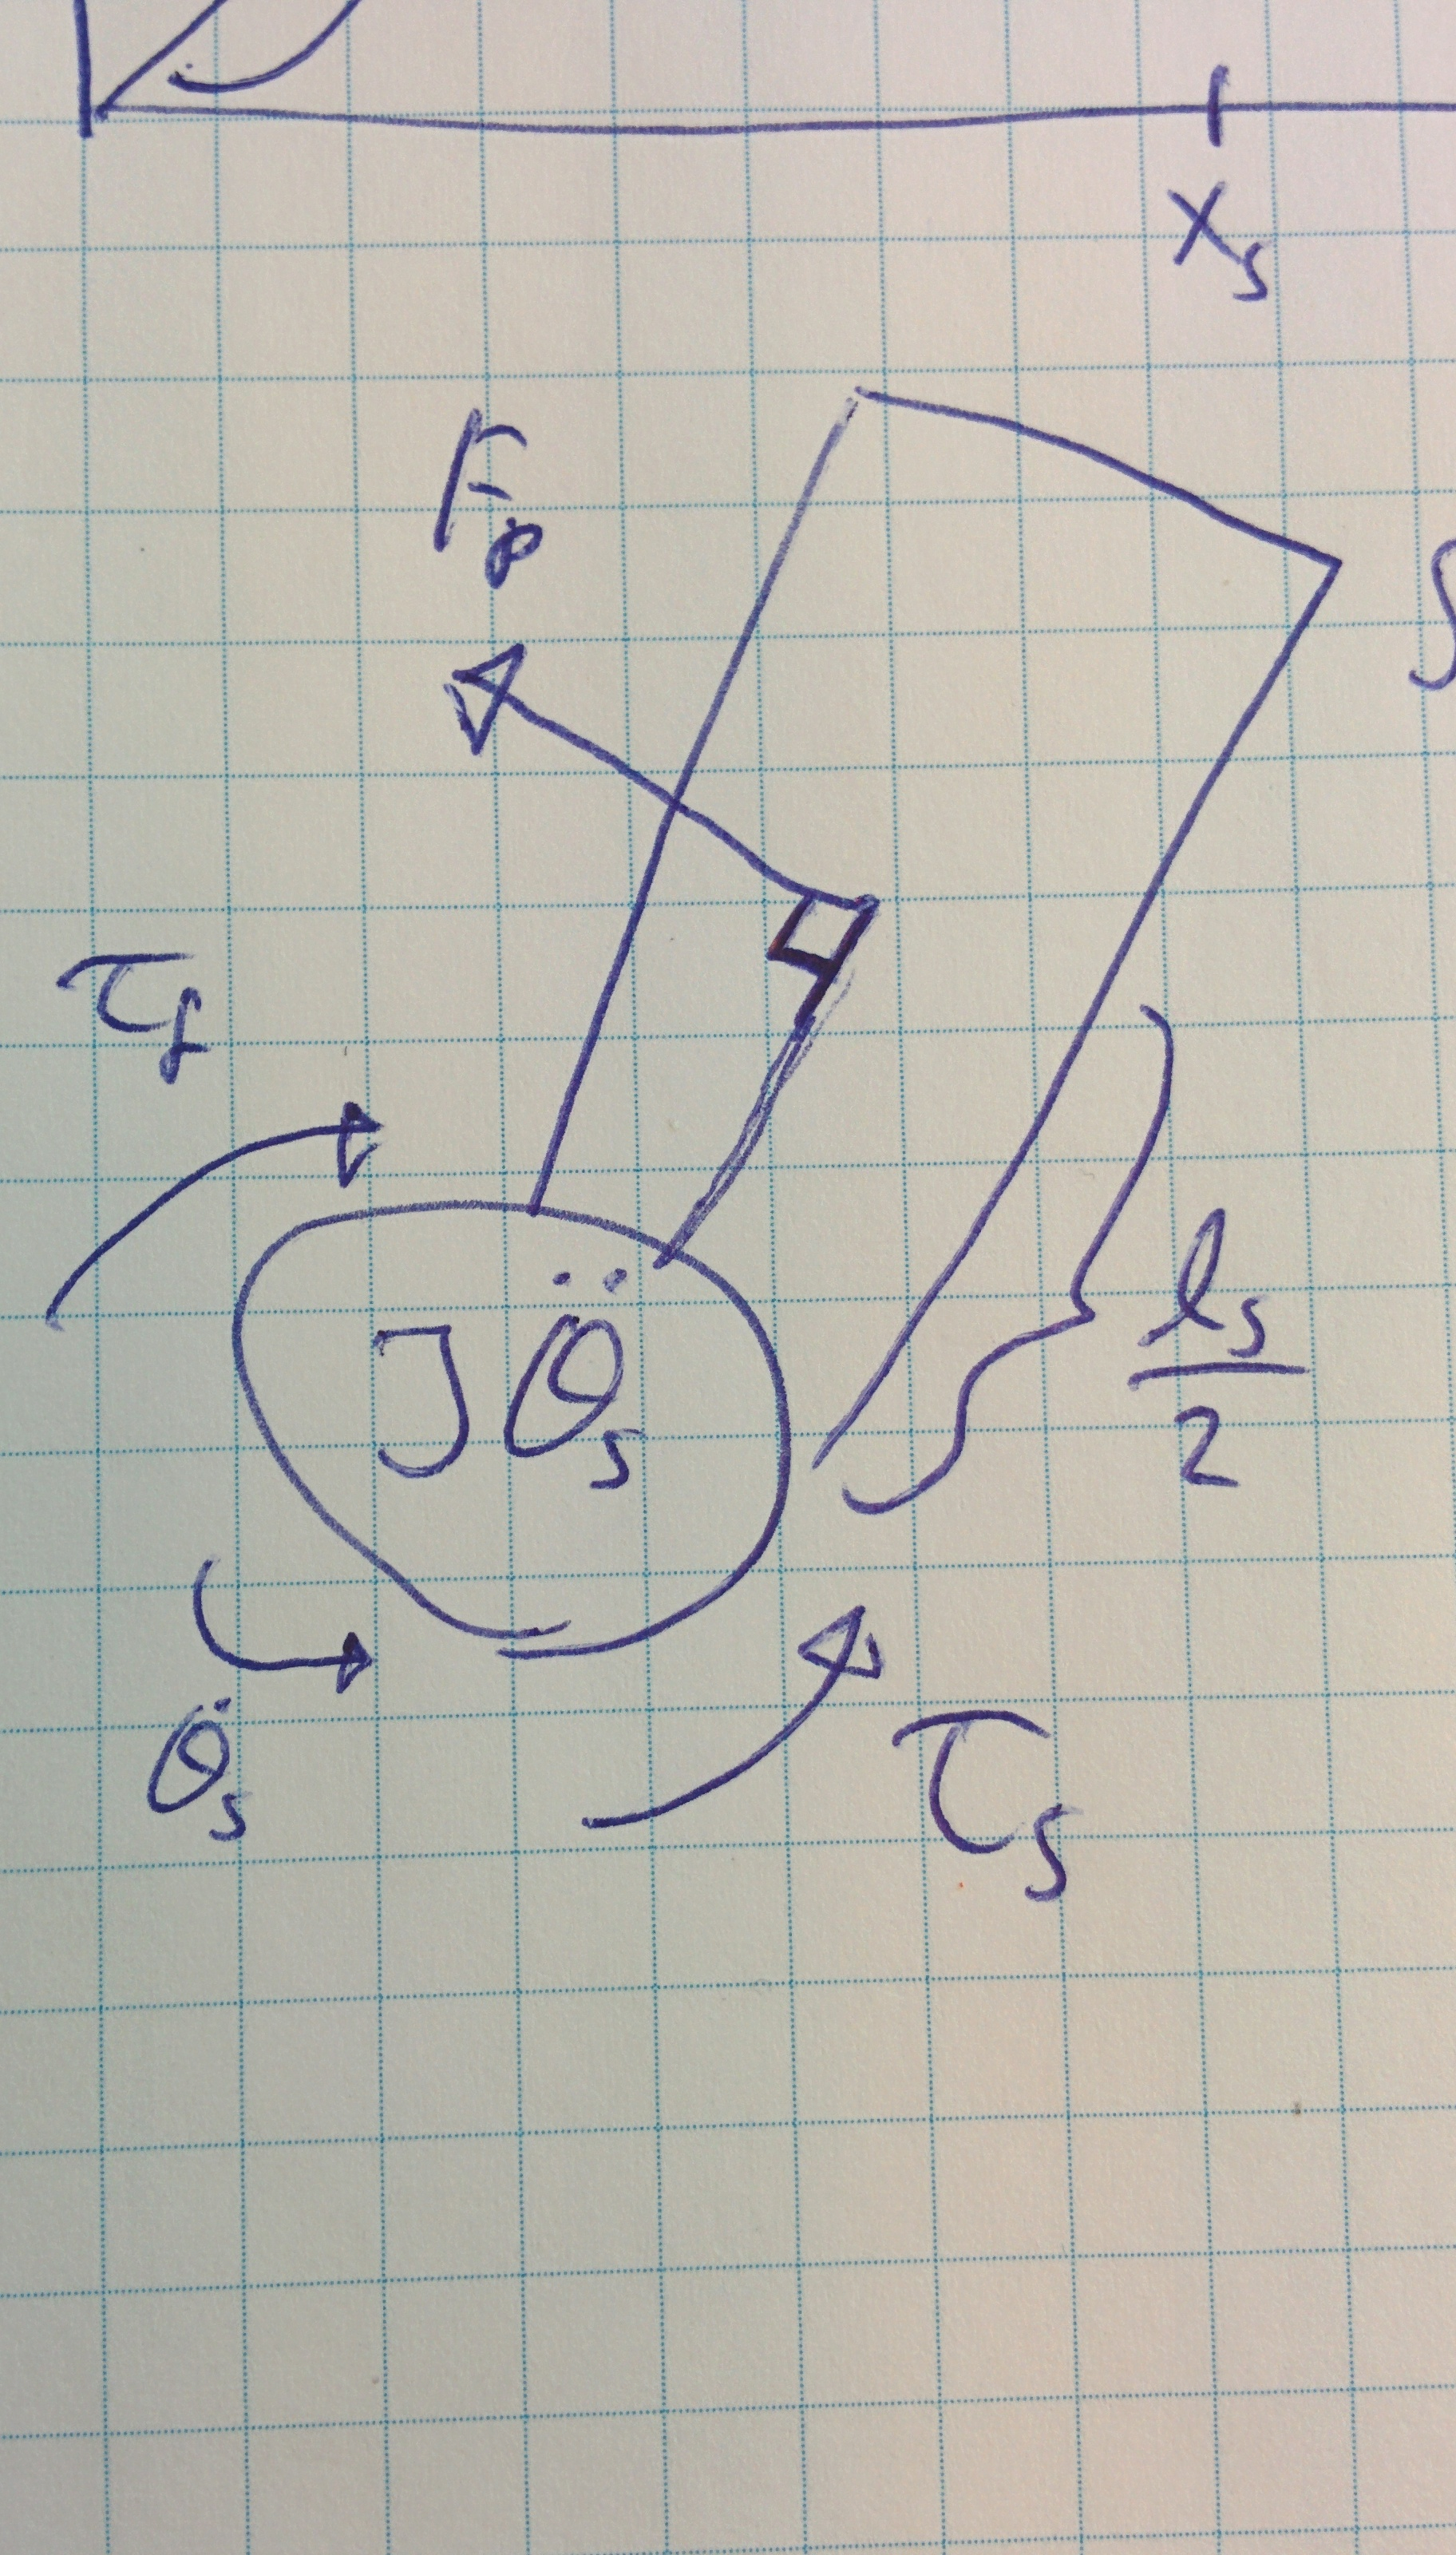
\includegraphics[width=0.25\textwidth]{FreeBodyPendulum}
		%\caption{Free body diagram of the joint that connects the arm and the stick.}
		%\label{fig:freebodystick}
		%\end{figure}
		%\todo[inline, author=Jacob]{Make pretty graph}
		%
		%The moment of inertia for the joint is described by \autoref{eq:Jrthetas}.
		%\begin{subequations}
		%\begin{flalign}
		%& J_r\ddot{\theta}_s=\tau_s-\tau_f  \label{eq:Jrthetas} \\
		%& \tau_s =F_p\frac{l_s}{2} \\
		%& \tau_f =b_{as}\dot{\theta}_{as} 
		%\end{flalign}
		%\end{subequations}
		%\startexplain
		%	\explain{$J_r$ is the moment of inertia for the stick}{\si{\kg\square\meter}}
		%	\explain{$\ddot{\theta}_s$ is the angular acceleration of the stick}{\si{\radian\per\square\second}}
		%	\explain{$\tau_s$ is the torque induced by the rotation of the stick}{\si{\newton\meter}}
		%	\explain{$\tau_f$ is the torque of the friction acting on the stick}{\si{\newton\meter}}
		%	\explain{$F_p$ is the force perpendicular to the stick at the center of mass}{\si{\newton}}
		%	\explain{$b_{as}$ is the viscous friction coefficient between the arm and the stick}{\si{\newton\meter\second}}
		%	\explain{$\dot{\theta}_{as}$ is the difference in angular velocity between the arm and the stick ($\dot{\theta}_s-\dot{\theta}_a$)}{\si{\radian\per\second}}
		%\stopexplain
		%
		%The friction is calculated from the difference in angular velocity as the stick could be perfectly upright while the arm moves causing the joint to turn. The angle of the arm is not considered as producing a torque acting on the joint but as part of the force on the stick, $F_p$.
		
		The forces acting on the rocket in the x and y directions are found by \vref{eq:FxFyRocket} using Newton's 2nd law of motion. Unlike in the inverted pendulum, there is no reaction to gravity from the arm, thus gravity does not produce any torque.
		
		\begin{subequations}  \label{eq:FxFyRocket}
			\begin{flalign}
				& F_x=\ddot{x}_bM_b  \addunit{\newton}\\
				& F_y=\ddot{y}_bM_b  \addunit{\newton}\\
			\end{flalign}
		\end{subequations}
		\startexplain
		\explain{$M_b$ is the mass of the stick}{\si{\kilo\gram}}
		\stopexplain
		The position of the center of mass of the rocket in the x and y direction is found by \vref{eq:XbYbRocket} using geometry.
		\begin{subequations}\label{eq:XbYbRocket} 
			\begin{flalign}
				& x_b=l_t\sin (-\theta_t)+C_g \sin (-\theta_b) \\
				& x_b=-l_t\sin (\theta_t)-C_g \sin (\theta_b) \\
				& y_b = l_t\cos (-\theta_t)+C_g \cos(-\theta_b) \\
				& y_b = l_t\cos (\theta_t)+C_g \cos(\theta_b) 
			\end{flalign}
		\end{subequations}
		
		The derivatives of $x_b$ and $y_b$ are found in \vref{eq:derXbYbRocket}.
		\begin{subequations}\label{eq:derXbYbRocket} 
			\begin{flalign}
				\hspace{30pt} & \dot{x}_b=-l_t\dot{\theta}_t\cos(\theta_t)-C_g\dot{\theta}_b\cos(\theta_b) & [\si{\meter\per\second}] \\
				& \ddot{x}_b=-l_t\ddot{\theta}_t\cos(\theta_t)+l_t\dot{\theta}_t^2\sin(\theta_t)-C_g\ddot{\theta}_b\cos(\theta_b)+C_g\dot{\theta}_b^2\sin(\theta_b) & [\si{\meter\per\square\second}] \\
				& 
				\dot{y}_b=-l_t \dot{\theta}_t\sin(\theta_t)-C_g\dot{\theta}_b\sin(\theta_b) & [\si{\meter\per\second}] \\
				& \ddot{y}_b=-l_t\ddot{\theta}_t\sin(\theta_t)-l_t\dot{\theta}_t^2\cos(\theta_t)-C_g\ddot{\theta}_b\sin(\theta_b)-C_g\dot{\theta}_b^2\cos(\theta_b) & [\si{\meter\per\square\second}]
			\end{flalign}
		\end{subequations}
		
		The forces $F_x$ and $F_y$ can be decomposed into perpendicular and parallel forces at that point. The parallel forces are negligible when assuming the rocket is perfectly solid and unable to stretch or compress. The perpendicular forces are found by \vref{eq:perpFxFyRocket} and are seen on (figure to do).
		
		%\begin{figure}[htbp]
		%\centering
		%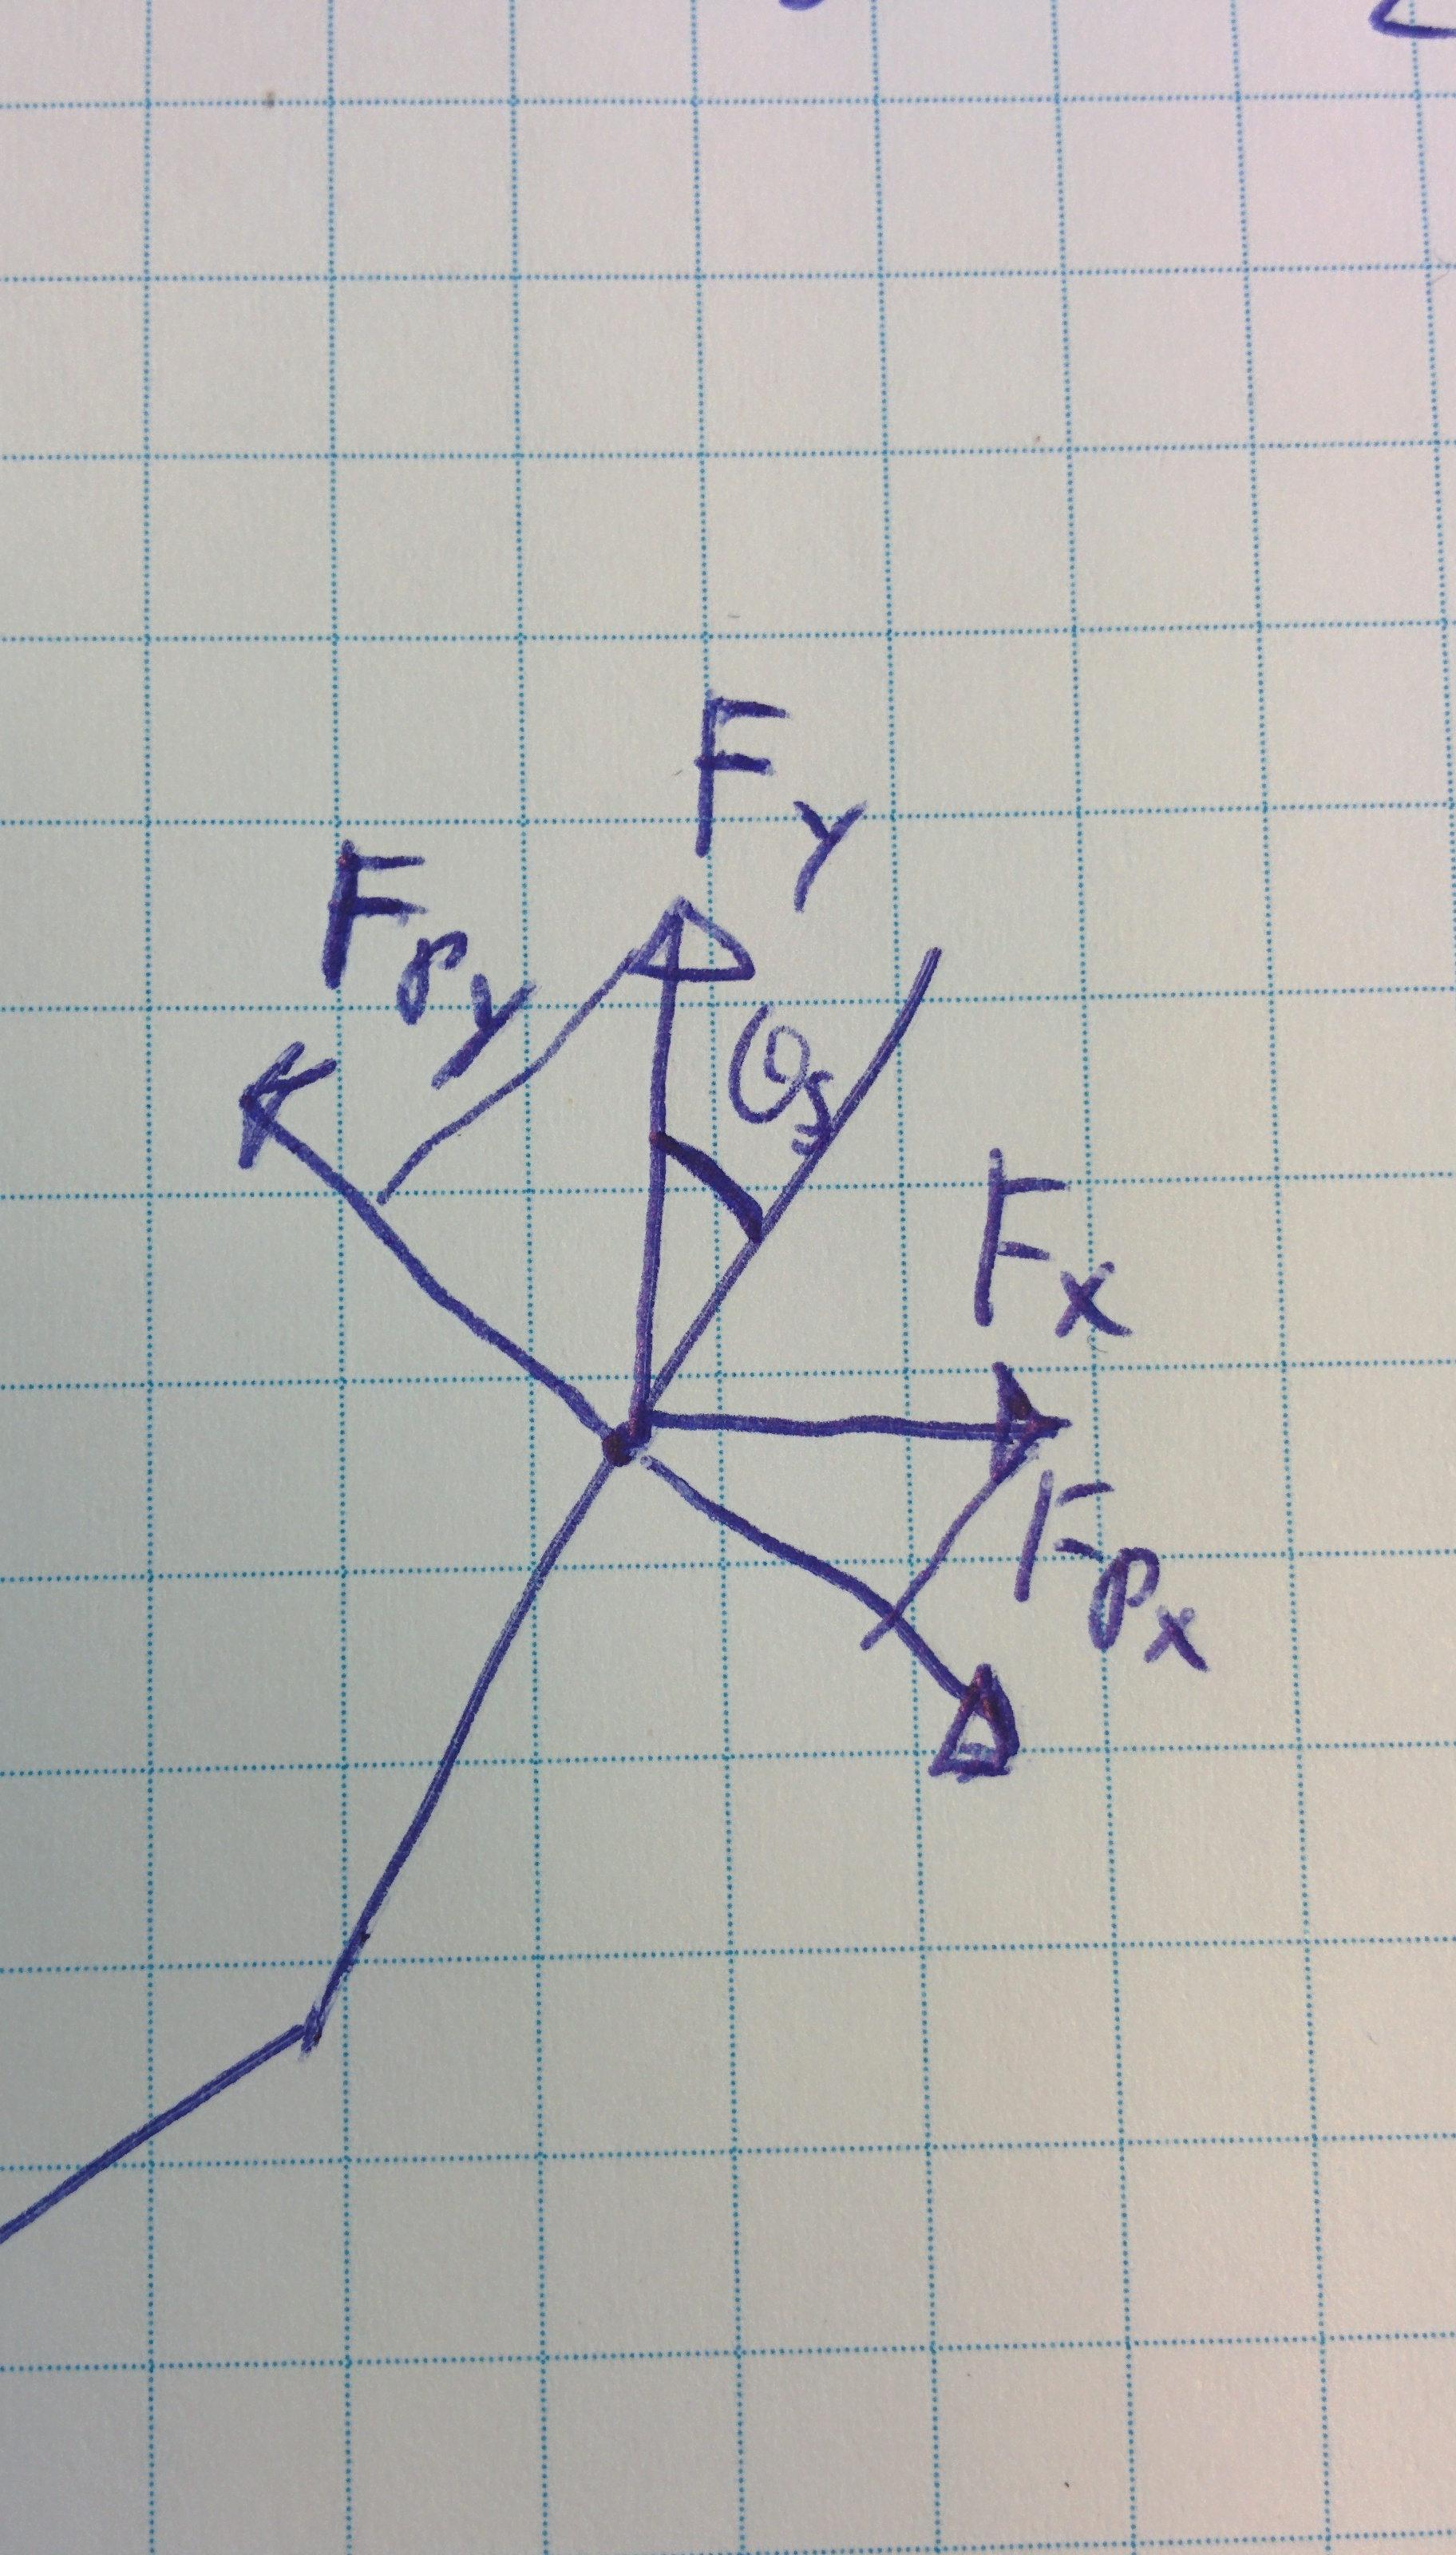
\includegraphics[width=0.25\textwidth]{ForcePerp}
		%\caption{Diagram of the forces, $F_x$ and $F_y$, decomposed into perpendicular forces.}
		%\label{fig:ForcePerp}
		%\end{figure}
		
		\begin{subequations}\label{eq:perpFxFyRocket}
			\begin{flalign}
				& F_{px}=F_x\cos(\theta_b) \\
				& F_{py}=F_y\sin(\theta_b)  \\
				& F_p = F_{px}+F_{py} 
			\end{flalign}
		\end{subequations}
		
		The rotary force of the rocket is described by \vref{eq:JrLongRocket}.
		\begin{subequations}
			\begin{flalign}
				J_r\ddot{\theta}_b &=C_g\left(F_x\cos(\theta_b)+F_y\sin(\theta_b)\right)-b_{tb}\dot{\theta}_{tb}  \\
				J_r\ddot{\theta}_b = C_g \cdot M_b \Big( &-l_t\ddot{\theta}_t\left(\cos(\theta_t)\cos(\theta_b)+\sin(\theta_t)\sin(\theta_b)\right) \notag \\
				& +l_t\dot{\theta}_t^2\left(\sin(\theta_t)\cos(\theta_b)-\cos(\theta_t)\sin(\theta_b)\right) \notag \\
				& -C_g\ddot{\theta}_b\left(\cos(\theta_b)\cos(\theta_b)+\sin(\theta_b)\sin(\theta_b)\right) \notag \\
				& +C_g\dot{\theta}_b^2\left(\sin(\theta_b)\cos(\theta_b)-\cos(\theta_b)\sin(\theta_b)\right)  \notag \Big)-b_{tb}\dot{\theta}_{tb} \label{eq:JrLongRocket}
			\end{flalign}
		\end{subequations}
		
		Using the trigonometric properties in \vref{eq:trigprop}, \autoref{eq:JrLongRocket} is reduced to \vref{eq:JrShortRocket}.
		\begin{subequations} \label{eq:trigprop}
			\begin{flalign}
				& \cos(\theta_t)\cos(\theta_b)\pm \sin(\theta_t)\sin(\theta_b)=\cos(\theta_t \mp \theta_b)  \\
				& \sin(\theta_t)\cos(\theta_b)\pm \cos(\theta_t)\sin(\theta_b) = \sin(\theta_t \pm \theta_b) \\ 
				& \cos(\theta_b)^2+\sin(\theta_b)^2=1 
			\end{flalign}
		\end{subequations}
		\begin{flalign}
			J_r\ddot{\theta}_b = C_gM_b \Big( &-l_t\ddot{\theta}_t \cos(\theta_t-\theta_b)+l_t\dot{\theta}_t^2 \sin(\theta_t-\theta_b) \notag \\
			&-C_g\ddot{\theta}_b \Big)-b_{tb}\dot{\theta}_{tb} \label{eq:JrShortRocket}
		\end{flalign}
		
		This is the nonlinear mathematical model for the system. This will be linearized in order to perform a Laplace transformation. The linearization is made with a 1st order Taylor approximation. The linearization is done at the equilibrium point where the arm is in an upright position i.e. $\theta_b=0$. In the equilibrium point the derivatives of all the inputs and outputs are 0. In this case the inputs and outputs are $\theta_t$ and $\theta_b$ and the operating point is $\bar{\theta}_t=0$ and $\bar{\theta}_b=0$. The nonlinear model is expressed as a function of the inputs and outputs as seen in \vref{eq:nonLinearModelRocket}.
		\begin{flalign}\label{eq:nonLinearModelRocket}
			f\left(\theta_t, \dot{\theta}_t, \ddot{\theta}_t, \theta_b, \ddot{\theta}_b\right)=C_gM_b \Big( &-l_t\ddot{\theta}_t \cos(\theta_t-\theta_b)+l_t\dot{\theta}_t^2 \sin(\theta_t-\theta_b) \notag \\
			&-C_g\ddot{\theta}_b \Big)-b_{tb}\dot{\theta}_{tb}-J_r\ddot{\theta}_b
		\end{flalign}
		
		Generally all equilibriums can be found by setting \vref{eq:nonLinearModelRocket} equal to 0 and the derivatives to 0, and solving for $\theta_t=\bar{\theta}_t$ and $\theta_b=\bar{\theta}_b$. For the rocket the only two equilibriums are the rocket body pointing straight up and straight down. In this project only the postion with the nose pointing straight up is relevent. 
		
		The 1st order Taylor approximation of an equation with multiple variables is seen in \vref{eq:1stTaylor}.
		\begin{flalign}
			f\left(\theta_t, \dot{\theta}_t, \ddot{\theta}_t, \theta_b, \ddot{\theta}_b\right) & \approx f\left(\bar{\theta}_t, 0, 0, \bar{\theta}_b, 0\right) + \left. \frac{\partial f}{\partial \theta_t}\right|_{(\bar{\theta}_t, \bar{\theta}_b)} \hat{\theta}_t \notag \\
			& \phantom{=} + \left. \frac{\partial f}{\partial \dot{\theta}_t}\right|_{(\bar{\theta}_t, \bar{\theta}_b)} \hat{\dot{\theta}}_t + \left. \frac{\partial f}{\partial \ddot{\theta}_t}\right|_{(\bar{\theta}_t, \bar{\theta}_b)} \hat{\ddot{\theta}}_t \notag \\
			& \phantom{=} + \left. \frac{\partial f}{\partial \theta_b}\right|_{(\bar{\theta}_t, \bar{\theta}_b)} \hat{\theta}_b + \left. \frac{\partial f}{\partial \ddot{\theta}_b}\right|_{(\bar{\theta}_t, \bar{\theta}_b)} \hat{\ddot{\theta}}_b \label{eq:1stTaylor}
		\end{flalign}
		\startexplain
		\explain{$\bar{\theta}$ denotes the angle in an operating point}{\si{\radian}}
		\explain{$\hat{\theta}$ denotes the angle of the small signal variances}{\si{\radian}}
		\stopexplain
		
		The three terms with sin or cos in \vref{eq:JrShortRocket} will be approximated individually using \vref{eq:1stTaylor}, remembering that $\bar{\theta}=\bar{\dot{\theta}}=\bar{\ddot{\theta}}=0$ in the equilibrium state.
		\begin{subequations}
			\begin{flalign}
				-l_t\ddot{\theta}_t\cos\left(\theta_t-\theta_b\right)  \approx & \ 0 + l_t\bar{\ddot{\theta}}_t\sin\left(\bar{\theta}_t-\bar{\theta}_b\right)\hat{\theta}_t  \notag \\ 
				& -l_t\cos\left(\bar{\theta}_t-\bar{\theta}_b\right)\hat{\ddot{\theta}}_t - l_t\bar{\ddot{\theta}}_t\sin\left(\bar{\theta}_t-\bar{\theta}_b\right)\hat{\theta}_b   \\
				-l_t\ddot{\theta}_t\cos\left(\theta_t-\theta_b\right) \approx &-l_t\hat{\ddot{\theta}}_t 
			\end{flalign} %\bar{\ddot{\theta}}_b
		\end{subequations}
		\begin{subequations}
			\begin{flalign}
				l_t\dot{\theta}_t^2\sin\left(\theta_t-\theta_b\right)  \approx &\ 0 + l_t\bar{\dot{\theta}}_t^2\cos\left(\bar{\theta}_t-\bar{\theta}_b\right)\hat{\theta}_t  \notag \\
				& + 2l_t\bar{\dot{\theta}}_t\sin\left(\bar{\theta}_t-\bar{\theta}_b\right)\hat{\dot{\theta}}_t-l_t\bar{\dot{\theta}}_t^2\cos\left(\bar{\theta}_t-\bar{\theta}_b\right)\hat{\theta}_b   \\
				l_t\dot{\theta}_t^2\sin\left(\bar{\theta}_t-\bar{\theta}_b\right) \approx & \ 0 
			\end{flalign}
		\end{subequations}
		
		Inserting the linearized terms in \vref{eq:JrShortRocket} and using the moment of inertia for a rotating stick, $J_r=\frac{1}{12}M_sl_s^2$, the linearized model becomes \eqref{eq:JrFinalRocket}.
		\begin{subequations}
			\begin{flalign}
				& \frac{1}{12}M_bl_b^2\hat{\ddot{\theta}}_b= M_b\left(-l_t\hat{\ddot{\theta}}_t-C_g\hat{\ddot{\theta}}_b+g\hat{\theta}_b\right)-b_{tb}\hat{\dot{\theta}}_{tb}   \\
				& \frac{1}{12}M_bl_b^2\hat{\ddot{\theta}}_b+\frac{1}{4}M_bl_b^2\hat{\ddot{\theta}}_b=C_gM_b\left(-l_t\hat{\ddot{\theta}}_t+g\hat{\theta}_b\right)-b_{tb}\hat{\dot{\theta}}_{tb}   \\
				& \frac{1}{3}M_bl_b^2\hat{\ddot{\theta}}_b=C_gM_b\left(-l_t\hat{\ddot{\theta}}_t+g\hat{\theta}_b\right)-b_{tb}\hat{\dot{\theta}}_{tb}  \label{eq:TauSmLin} \\
				& \hat{\ddot{\theta}}_b=\frac{3}{2l_b}\left(-l_t\hat{\ddot{\theta}}_t+g\hat{\theta}_b\right)-\frac{3b_{tb}\left(\hat{\dot{\theta}}_b-\hat{\dot{\theta}}_t\right)}{M_bl_b^2} \label{eq:JrFinalRocket}
			\end{flalign}
		\end{subequations}
		
		The linearized model is now Laplace transformed in \autoref{eq:tfArmStick} in order to find the transfer function.
		\begin{subequations}
			\begin{flalign}
				& s^2\Theta_b=\frac{3}{2l_b}\left(-s^2l_t\Theta_t+g\Theta_b\right)-s\frac{3b_{tb}}{M_bl_b^2}\Theta_b+s\frac{3b_{tb}}{M_bl_b^2}\Theta_t  \\
				& \Theta_b\left(s^2+\frac{3b_{tb}}{M_bl_b^2}s-\frac{3g}{2l_b}\right)=\Theta_t\left(-\frac{3l_t}{2l_b}s^2+\frac{3b_{tb}}{M_bl_b^2}s\right)  \\
				& \frac{\Theta_b}{\Theta_t}=-\frac{\frac{3l_t}{2l_b}s^2-\frac{3b_{tb}}{M_bl_b^2}s}{s^2+\frac{3b_{tb}}{M_bl_b^2}s-\frac{3g}{2l_b}} \label{eq:tfArmStick}
			\end{flalign}
		\end{subequations}
		
		A linearized model in the Laplace domain for the arm and the stick has been derived and the model for the gears is now derived.





\chapter{Requirements and Specifications}
The following chapter describes requirements and specifications that is determined for controlling both the rocket and the inverted pendulum. The requirements is set to obtain a system which fulfils the problem statement \todo{Ref to section - Mathias and might be changed in formulation}.

As described earlier the goal of both systems is to react to deviations from its stable position. The goal of the rocket is the launch and fly stable and straight versus the inverted pendulum where the goal is to balance the stick in vertical upwards position.  

Both systems will be described with physical and control requirements in separate sections. The physical requirements will be set based on the limits of the models. Where the requirements for the controllers will be set based on the approximations of best possible control parameters for each model.  
The controller requirements will be approximated based on speed, precision and stability, which means that following control parameters would be set for:

\begin{itemize}[noitemsep]
\item Settling Time
\item Overshoot
\item Rise Time
\item Steady State Error
\end{itemize}

Each parameter would affect each other, and therefore a discussion of the best combination of them will be considered.

\subsection{Requirements for the Inverted Pendulum}
The requirements is based on figure \ref{fig:InvertedPendulumSetUp} where the angle relations and positions is described between the arm and stick.

 
Physical requirements:


The control position of the arm must not exceed $\pm$ 45$^{\circ}$. \todo{Maybe less is better, so that it isn't to different from rocket.}


Deviation from the upright position of the stick must not exceed $\pm$ 5 $^{\circ}$ when considered balanced.\todo{Might be changed based on resolution and precision of potentiometer}


The system should be able to regain balance if an angle impulse of 10 $^{\circ}$ is applied, in form of a push on the stick.\todo{}  


The arms recovery angle of the stick, when dropped from upwards position, should be minimum $\pm$15 $^{\circ}$ \todo{Probably not necessary to consider.}


Control requirements:



\subsection{Requirements for the Rocket}
Based on the capability 
The physical dimensions of the rocket can not exceed:
\begin{table}[htbp]
\centering
\begin{tabular}{lll}
\hline
Parameter    & Value & Unit  \\ \hline
Length       & 0.25  & m     \\
Width        & 0.25  & m     \\
Height       & 0.5   & m     \\
Total volume & 0.03  & m$^3$ \\
Weight       & 0.3   & kg   
\end{tabular}
\caption{Maximum size and weight of the rocket.}
\label{RocketDimensions}
\end{table}


Deviation from the predetermined trajectory of the rocket must not exceed $\pm$10 $^{\circ}$.\todo{Might be changed based on resolution and precision of gyroscope, and quantified.}


The system should be able to regain its stability and direction if an angle impulse of 10 $^{\circ}$ is applied, in form of a external disturbance, on the rocket.  


\section{Acceptance Test Specification}	
TBD

\part{Design}\label{pt:design} 
\graphicspath{{figures/Design/IPController/}}
\chapter{Design of the Inverted Pendulum Controller}\label{sec:IPController}
\todo[inline,author=Jacob]{Start with a blockdiagram that has the actual transfer functions.}

The goal of the controller is to balance the stick in an upright position. The system is seen as a block diagram on \autoref{BlockSystemNoControl}. Which gives the transfer function seen in \autoref{eq:OneGeneralLoop}
\begin{figure}[htbp]
\centering
\missingfigure{}
\caption{Block diagram of the system the controller will attempt to stabilize.}
\label{fig:BlockSystemNoControl}
\end{figure}

\begin{equation}\label{eq:OneGeneralLoop}
	\frac{\Theta_s}{U}=\frac{0.0004341 s^2}{0.001559 s^4 + 0.002537 s^3 - 0.0204 s^2 - 0.03391 s}
\end{equation}

The system is inherently unstable as it is evident by the pole in the right half plane of the pole-zero plot in \autoref{fig:pzip}.

\begin{figure}[htbp]
\centering
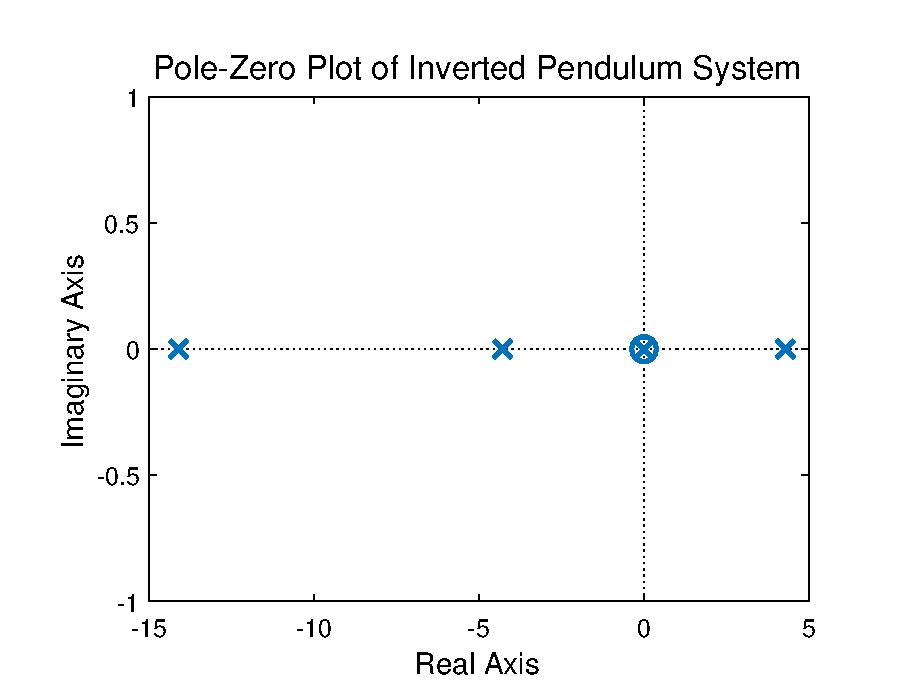
\includegraphics[width=0.6\textwidth]{pzip}
\caption{Pole-zero plot for the inverted pendulums transfer function.}
\label{fig:pzip}
\end{figure}
\todo[inline,author=Jacob]{Check constants found by test and transfer function at the end.}

The problem with the system is the unstable pole in the right half plane and the zeros in 0.

There's a plethora of different options for the controller to use; the simplest being a proportional controller. A simple way to check whether the proportional controller is feasible is by examining the root locus of the transfer function in \autoref{fig:locusIP}. The pole in the right half plane moving towards infinity is caused by the transfer function being negative and can be fixed with a negative gain as shown on figure \autoref{fig:locusNegative}.

\begin{figure}[htbp]
\centering
	\begin{subfigure}{0.45\textwidth}
	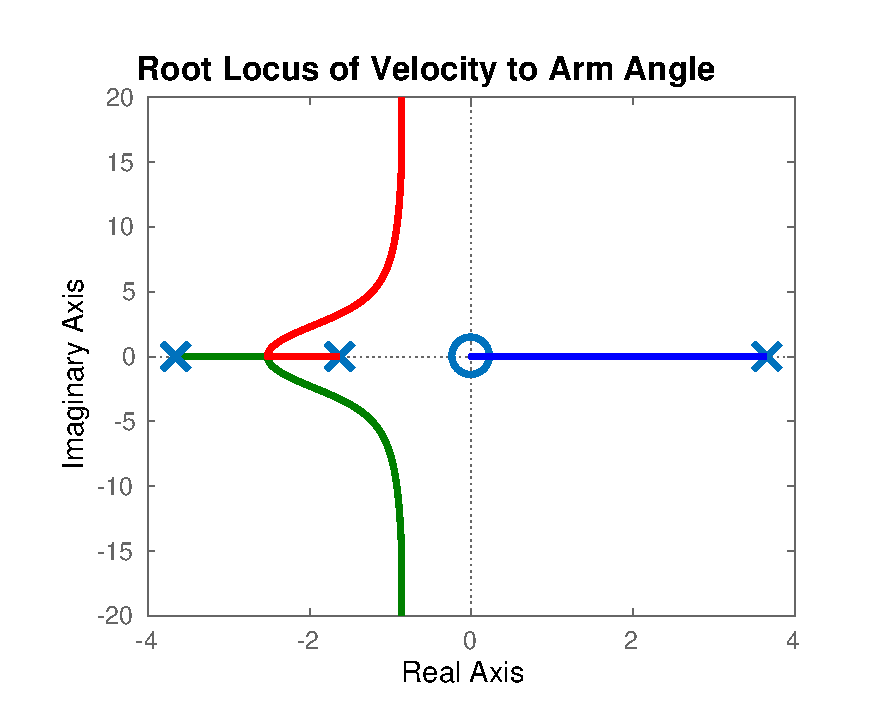
\includegraphics[width=\textwidth]{rlocusplus}
	\caption{Positive gain.}
	\label{fig:locusIP}
	\end{subfigure}
	\begin{subfigure}{0.45\textwidth}
	\centering
	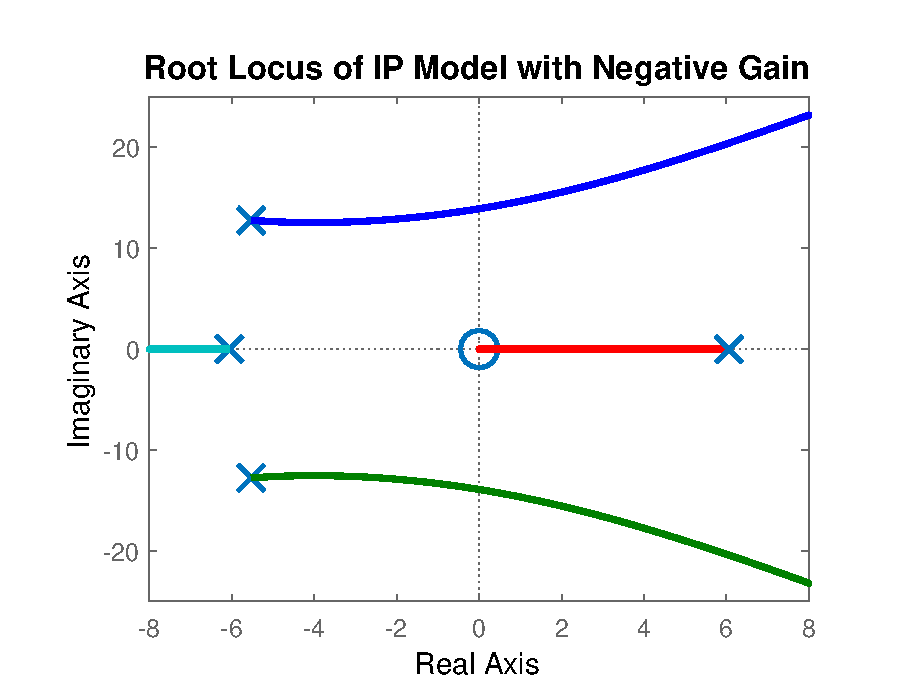
\includegraphics[width=\textwidth]{rlocusminus}
	\caption{Negative gain.}
	\label{fig:locusNegative}
	\end{subfigure}
\caption{Root locus of the inverted pendulums transfer function.}
\end{figure}

The proportional controller isn't feasible as the pole in the right half plane never enters the stable region even with a negative gain. This is because the pole will always end at a zero if available. The zero in 0 blocks the unstable pole from moving into the stable region.

The controller can be simplified by using cascade control. This means two controllers should be designed; one that controls the angle of the arm and one that controls the angle of the stick. The cascade control system can be seen on \autoref{fig:IPCascade}.

\begin{figure}[htbp]
\centering
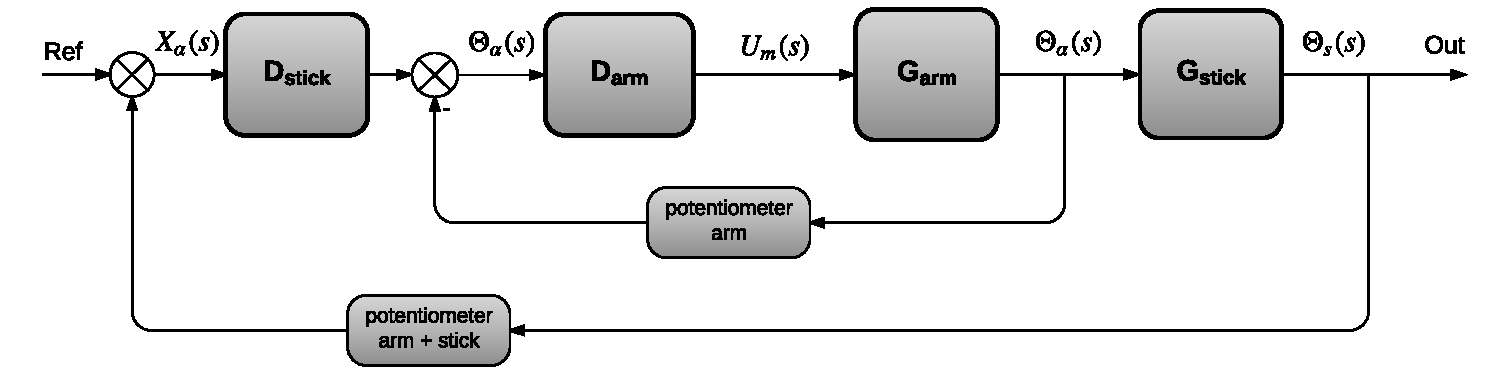
\includegraphics[width=\textwidth]{IPCascadeEnhanced}
\caption{Block diagram of the inverted pendulum system with cascade control.}
\label{fig:IPCascade}
\end{figure}

If the inner loop is fast enough compared to the outer loop, it is negligible to the outer loop controller. This means the root locus of the can be split into two separate systems with a respective controller that needs to be designed. These two new loops, which will be now referred as respectively inner loop and outer loop, have their transfer function define in \autoref{eq:InnerOuterTF}.

\begin{subequations}\label{eq:InnerOuterTF}
	\begin{flalign}
		\frac{\Theta_a}{U}&= \frac{0.0009648}{0.001559 s^2 + 0.002537 s + 0.0009648}\\
		\frac{\Theta_s}{\Theta_a}&=\frac{0.45 s^2}{1.45 s^2 - 13.36}
	\end{flalign}
\end{subequations}

The root locus of the two subsystems is seen on \autoref{fig:locusSplit}.
\begin{figure}[htbp]
\centering
	\begin{subfigure}{0.45\textwidth}
	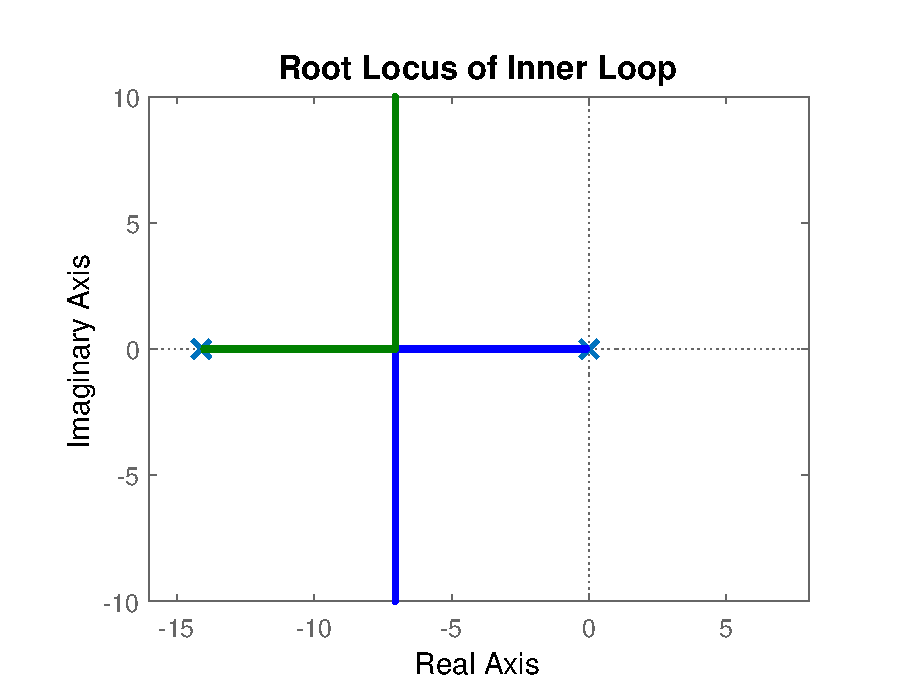
\includegraphics[width=\textwidth]{rlocusVArmAlt}
	\caption{Voltage as input and angle of the arm as output.}
	\label{fig:locusVArm}
	\end{subfigure}
	\begin{subfigure}{0.45\textwidth}
	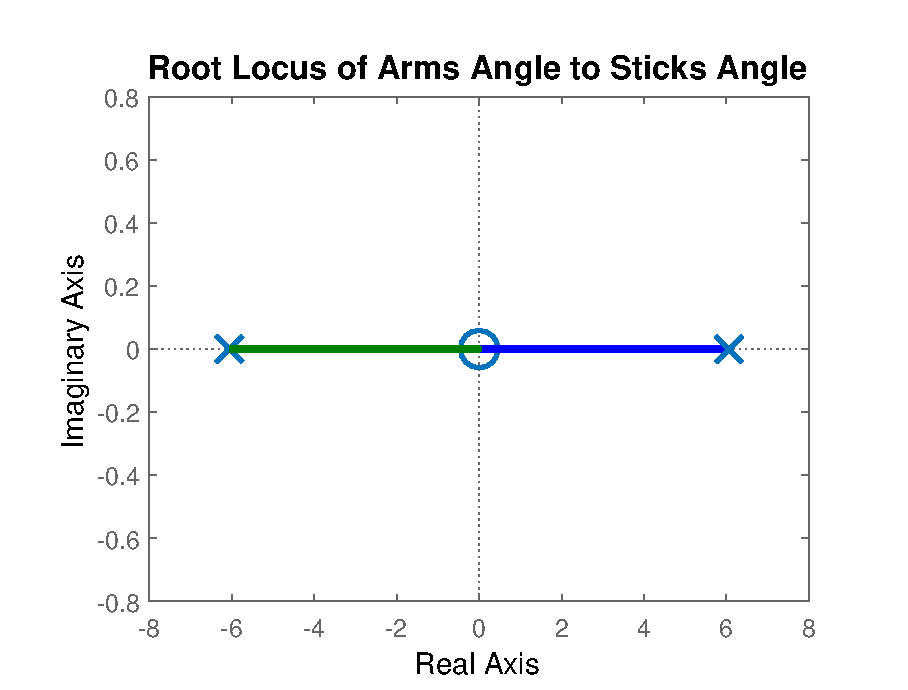
\includegraphics[width=\textwidth]{rlocusArmStick}
	\caption{Angle of the arm as input and angle of the stick as output.}
	\end{subfigure}
\caption{Root locus of the inner loop and outer loop.}
\label{fig:locusSplit}
\end{figure}

With this split it's simpler to design a controller that can move the unstable pole to the stable region. The inner loop controller will be designed first as it's essential to this split that the inner loop is faster than the outer loop. The inner loop controller will be designed to be as fast as possible before the outer loop controller is designed.

\section{Design of Inner Loop Controller}

For the design of the inner loop controller, it is important that it settles faster than the outer loop controller without any overshoot. This means the natural frequency of the system with the controller needs to be larger and the poles close to the real axis. The root locus for the motor to the arm on \autoref{fig:locusVArm} shows that a simple gain can not increase the natural frequency without have any overshoot. As such a P controller is chosen as it will increase the rise time and the settling time. With the help of \autoref{fig:VArmGeneralPControllerRLocus} a gain of 9.28 is chosen as it is the maximum gain obtainable without having any overshoot.

\begin{figure} [htbp] 
	\centering
	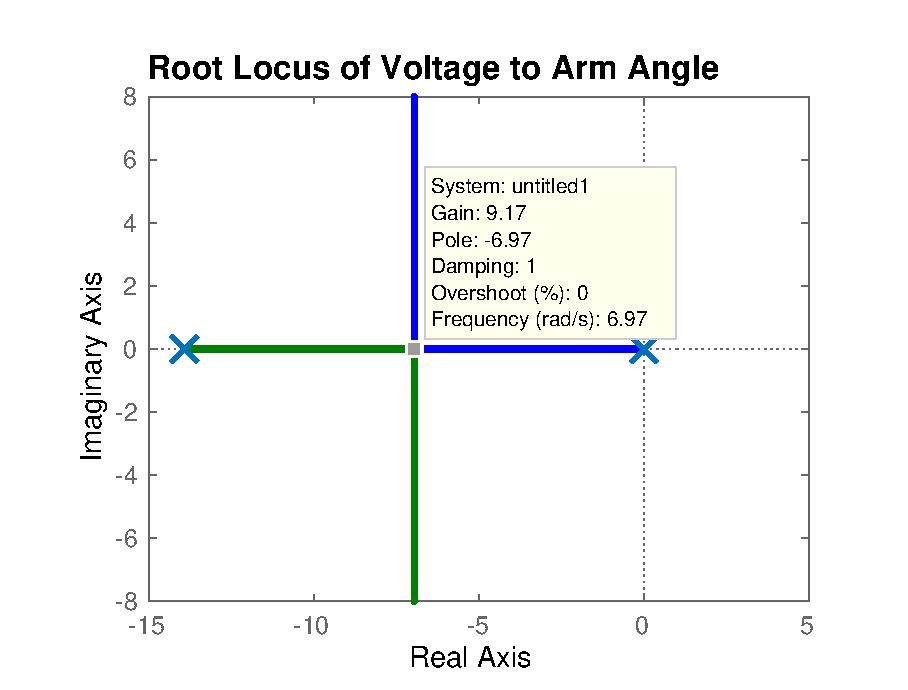
\includegraphics[width=0.7\textwidth]{rlocusVArmGeneralPController.eps}
	\caption{Voltage as input and Arm's angle as the output}
	\label{fig:VArmGeneralPControllerRLocus}
\end{figure}

However this system has only a natural frequency of \SI{6.97}{\radian\per\second} meaning the arm should be quite slow with this controller. This supposition is confirmed by the step response seen in \autoref{fig:VArmGeneralPControllerStepResp}.

\begin{figure} [htbp] 
	\centering
	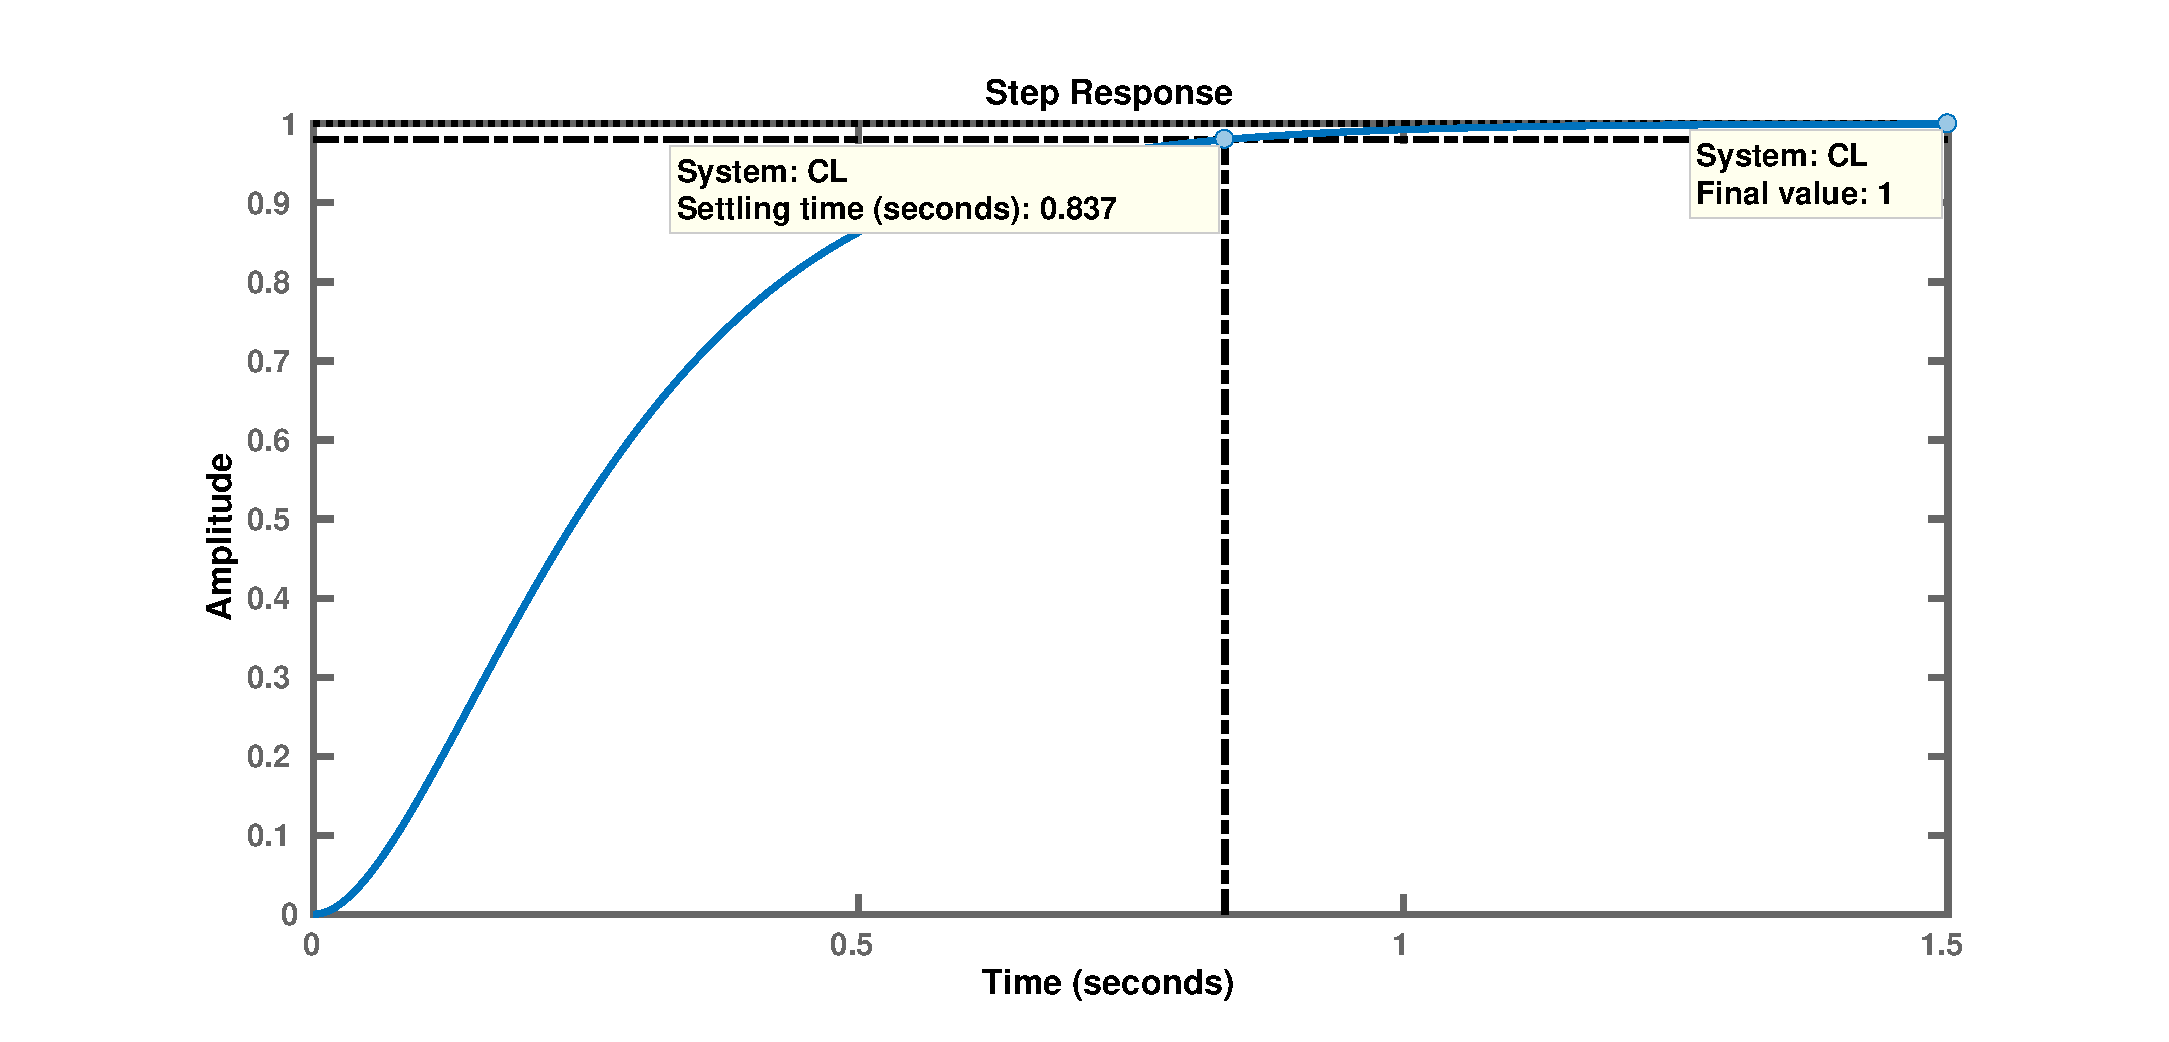
\includegraphics[width=0.8\textwidth]{rlocusVArmGeneralPControllerStepResp.eps}
	\caption{Step response of the arm with the voltage as the input}
	\label{fig:VArmGeneralPControllerStepResp}
\end{figure}

In order to speed up the inner loop two options are available. The first one is to use more elaborate controller than the P controller such as a PD controller or a lead. The second one is to once again divide the inner loop into two loops. The second method is chosen for two reasons. The first one is that since the motor has already a tachometer integrated, and so it is simpler to implement this method. The other one was a problem noticed during the test of the motor for its modeling. The driver is not delivering a constant speed for a constant voltage. And so a feedback loop of the velocity would be able to reduce the inconsistencies generated by the driver. The two new loops are respectively the voltage as the input and the velocity which will be called motor loop from now on, and the velocity as the input and the arm's angle as the output named as arm's loop.

The first loop which will be designed will be the motor loop as it is the most inner loop. The new control loop is added to \autoref{fig:IPCascade} to form the final block diagram presented in \autoref{fig:BlockAllLoops}.

\begin{figure}[htbp]
	\centering
	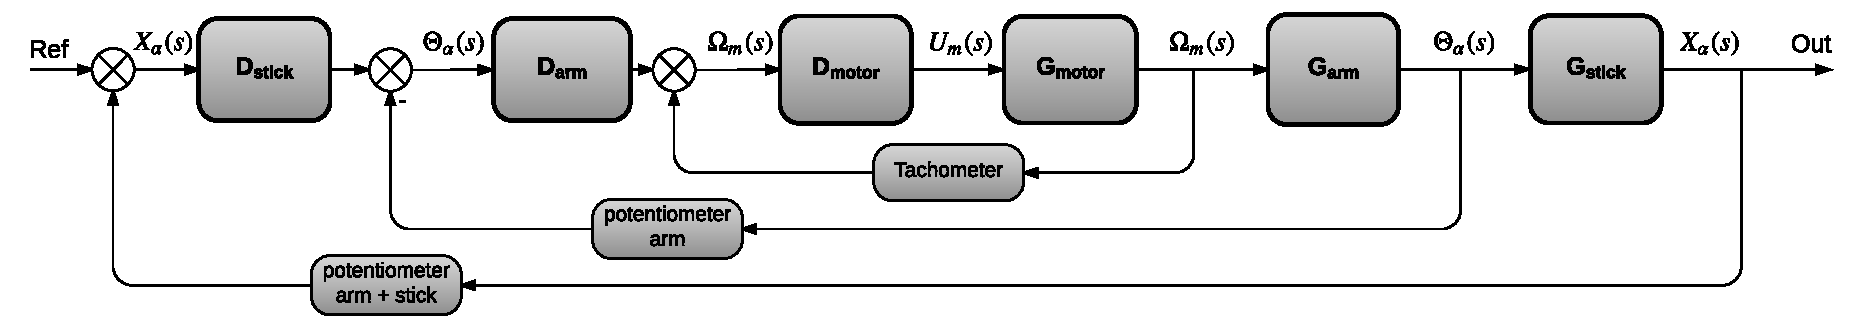
\includegraphics[width=\textwidth]{BlockAllLoops}
	\caption{New block diagram of the inverted pendulum system with cascade control.}
	\label{fig:BlockAllLoops}
\end{figure}

\input{chapters/Design/MotorLoop.tex}

\subsection{Design of the Arm Loop Controller}
Now the arm's loop will be designed. The motor loop part has a settling time of \SI{0.0159}{\second}, so the settling time of the arm's loop has to be at least \SI{0.159}{\second} in order to make the assumption that the motor's loop transfer function is equal to 1 for the arm's loop. The new transfer function derived from this approximation is \autoref{eq:WArmLoop}.

\begin{equation}\label{eq:WArmLoop}
	\frac{\Theta_a}{\Omega_m}=\frac{0.027}{s}
\end{equation}

The root locus of \autoref{eq:WArmLoop}, in \autoref{fig:WArmLoopRLocus}, shows that there is theoretically no gain limitation for the arm as the pole moves to the left side plan making the system stable, as long as the gain is high enough. The pole is also always on the real axis which means there will be no overshoot no matter the gain.

\begin{figure} [htbp] 
	\centering
	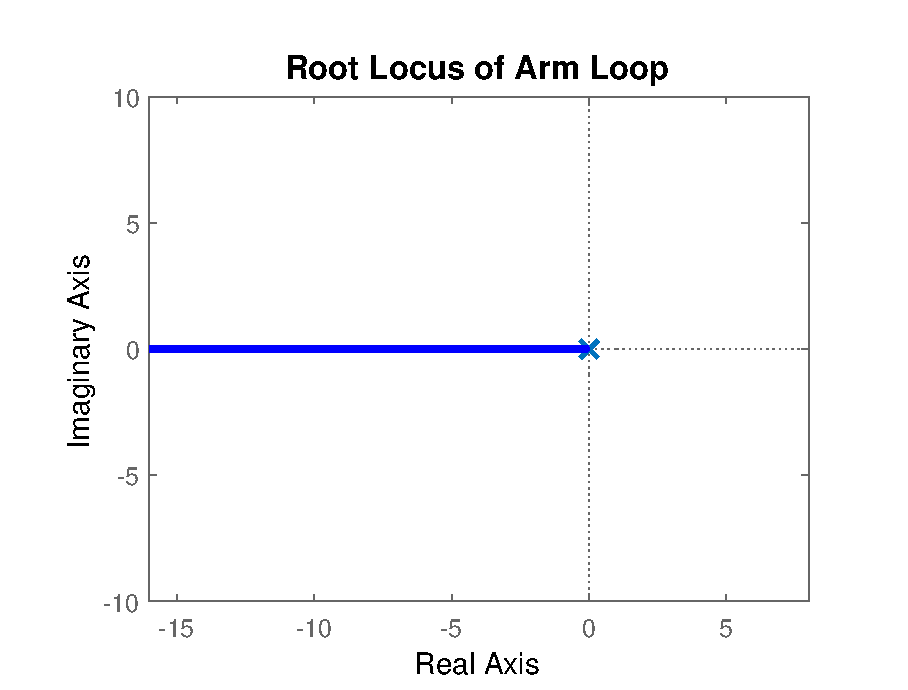
\includegraphics[width=0.7\textwidth]{WArmPControllerRLocus.eps}
	\caption{Velocity as input and Arm's angle as the output}
	\label{fig:WArmLoopRLocus}
\end{figure}

Since it is so our only limitation is the settling time of the motor as explained earlier. A gain of 905 is good enough as it gives a settling time of \SI{0.16}{\second} as seen in \autoref{fig:WArmLoopStepResp}.

\begin{figure} [htbp] 
	\centering
	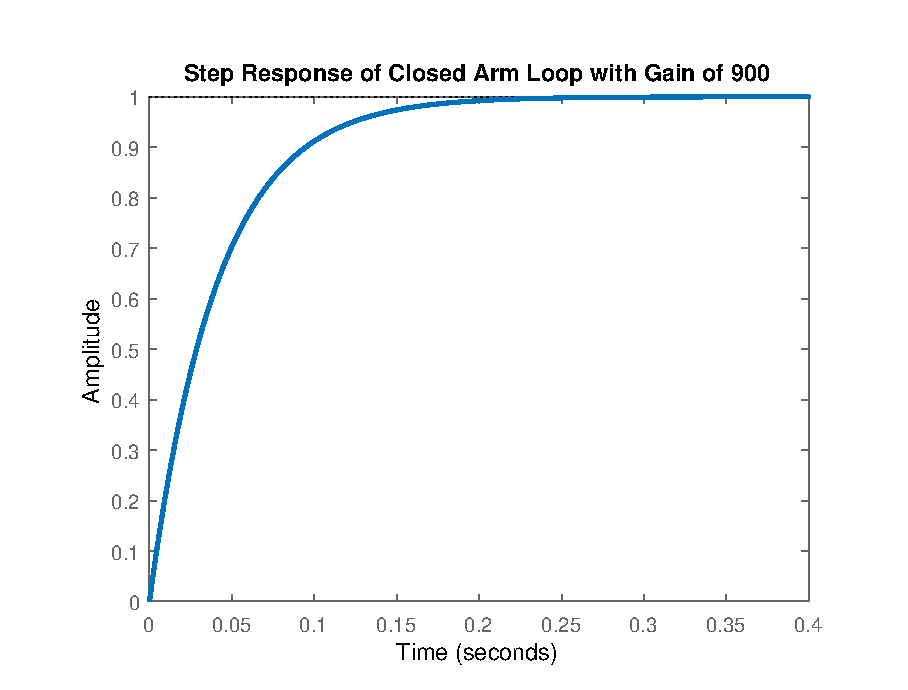
\includegraphics[width=0.8\textwidth]{WArmPControllerStepResp.eps}
	\caption{Step response of the arm's loop}
	\label{fig:WArmLoopStepResp}
\end{figure}

%By moving the zero further into the left half plane gives a faster settling time but requires a higher gain and a faster sampling rate for a digital controller. Having a higher gain can give issues with saturating the motor and there may be limits from the sampling rate with very fast settling times. 

\todo[inline,author=Jacob]{Maybe look into PID as it adds two zeros and is a well documented type of controller. Especially because lead control gives steady state error and the integration can remove it. SSE is terrible for the inner loop but ok for the outer as it's the position and not the angle.}


\section{Design of Outer Loop Controller}
As the poles in feedback will eventually end up at the zeros with a large enough gain, there are two options to bring the unstable pole into the stable region: Remove all zeros in 0 so the pole can cross the into the stable region along the real axis or add another unstable open loop pole to force the poles off the real axis and then try to circumvent the zeros in 0. 

Removing the zeros in 0 can't be done by adding poles as $\infty \cdot 0$ isn't defined. Instead it's better to try and redefine the model output to something with a DC gain but at the same time requires the stick to be balanced to achieve the new output. This could be by attempting to control the position of a point on the stick. The stick would need to be balanced in order to have the point always be in the correct position.

%Cancelling zeros in 0 by adding poles can be dangerous as the steady state error will no longer be zero which is critical for a stable inverted pendulum. The system is difficult to control as the transfer function was derived with an attempt to control the angle of the stick. This is only really possible in the special case where the reference is exactly 0 at all times. The system can instead be redefined as trying to control the position of a point on the stick in relation to the vertical axis. By controlling the position instead of the angle would mean the system would still have to balance the stick but not be forced to use a reference of 0 at all times. This could make the system easier to control.

\subsection{Redefining the Inverted Pendulums Output}
The inverted pendulum model will be redefined so the output is the distance from a point on the stick to the vertical axis instead of the angle of the stick. The point, $\alpha$, and the distance to the vertical axis, $x_\alpha$, are seen on \autoref{fig:modelDist}.

\begin{figure}[htbp]
\centering
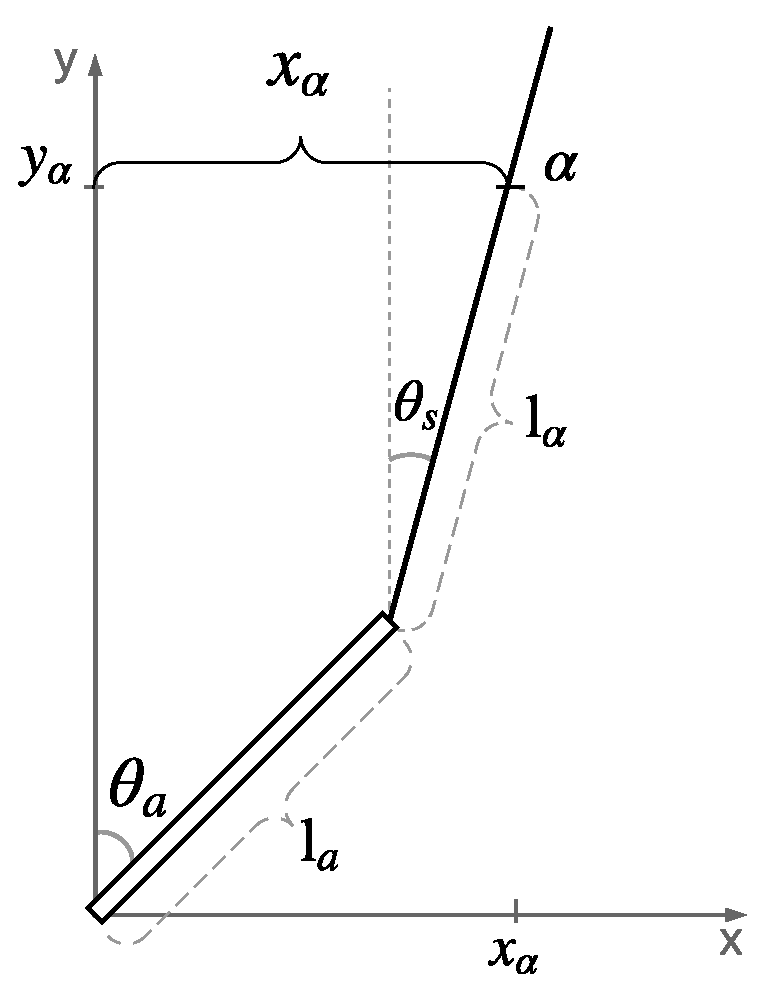
\includegraphics[width=0.5\textwidth]{ModelDistAlpha}
\caption{Diagram of the distance that will be controlled instead of the angle of the stick.}
\label{fig:modelDist}
\end{figure}

The distance to the point can be described by \autoref{eq:xa}.
\begin{flalign}\label{eq:xa}
& x_\alpha(t) = l_a\sin(\theta_a(t))+l_\alpha\sin(\theta_s(t))
\end{flalign}
This is not a linear equation and needs to be linearized in order to Laplace transform it. This is done with a 1st order Taylor approximation around the equilibrium where $\theta_a=\theta_s=0$ in \autoref{eq:xaTaylor}
\begin{subequations}\label{eq:xaTaylor}
\begin{flalign}
& x_\alpha(t)\approx l_a\sin(0)+l_a\cos(0)\theta_a(t)+l_\alpha\sin(0)+l_\alpha\cos(0)\theta_s(t) \\
& x_\alpha(t)\approx l_a\theta_a(t)+l_\alpha\theta_s(t)
\end{flalign}
\end{subequations}
This will then be Laplace transformed in \autoref{eq:xaLaplace}.
\begin{flalign}\label{eq:xaLaplace}
X_\alpha(s)=l_a\Theta_a(s)+l_\alpha\Theta_s(s) 
\end{flalign}

By isolating $\Theta_s(s)$ in \autoref{eq:tfArmStick} and inserting it into \autoref{eq:xaLaplace}, the transfer function in \eqref{eq:xatf} is found. The friction part is removed per \autoref{tab:IPModelVar}.

\begin{subequations}
\begin{flalign}
& X_\alpha(s)=l_a\Theta_a(s)+l_\alpha\frac{-\frac{3l_a}{2l_s}s^2}{s^2-\frac{3g}{2l_s}}\Theta_a(s) \\
& X_\alpha(s)=\frac{l_a\left(s^2-\frac{3g}{2l_s}\right)+l_\alpha\left(-\frac{3l_a}{2l_s}s^2\right)}{s^2-\frac{3g}{2l_s}}\Theta_a(s) \\
& \frac{X_\alpha(s)}{\Theta_a(s)} = \frac{s^2\left(l_a-l_\alpha\frac{3l_a}{2l_s}\right)-l_a\frac{3g}{2l_s}}{s^2-\frac{3g}{2l_s}} \label{eq:xatf}
\end{flalign}
\end{subequations}
The transfer function still ends up with 2 zeros but it's possible to remove them by selecting the point $\alpha$ so $l_\alpha=\frac{2l_s}{3}$. Inserting this into \autoref{eq:xatf} the transfer function becomes \autoref{eq:xaTF}.
\begin{flalign}\label{eq:xaTF}
& \frac{X_\alpha(s)}{\Theta_a(s)} = \frac{-l_a\frac{3g}{2l_s}}{s^2-\frac{3g}{2l_s}}
\end{flalign}

The zeros in 0 has been removed but the distance, $x_\alpha$, now needs to be measured for the feedback. This can be done by measuring the angles, which was also necessary before, but now use \autoref{eq:xa} to calculate the distance instead of using the angle directly. The controller for the transfer function in \autoref{eq:xaTF} can now be designed.
\subsection{Controlling the Distance from the Stick to Vertical}
%The controller for the system will be split into two. One controller in an inner loop that controls the angle of the arm and one in an outer loop that controls the position of the stick. The system with the two controllers can be seen on the block diagram on \autoref{fig:IPBlock}.
%
The new block diagram for the controllers can be seen on \autoref{fig:IPBlock}.
\begin{figure}[htbp]
\centering
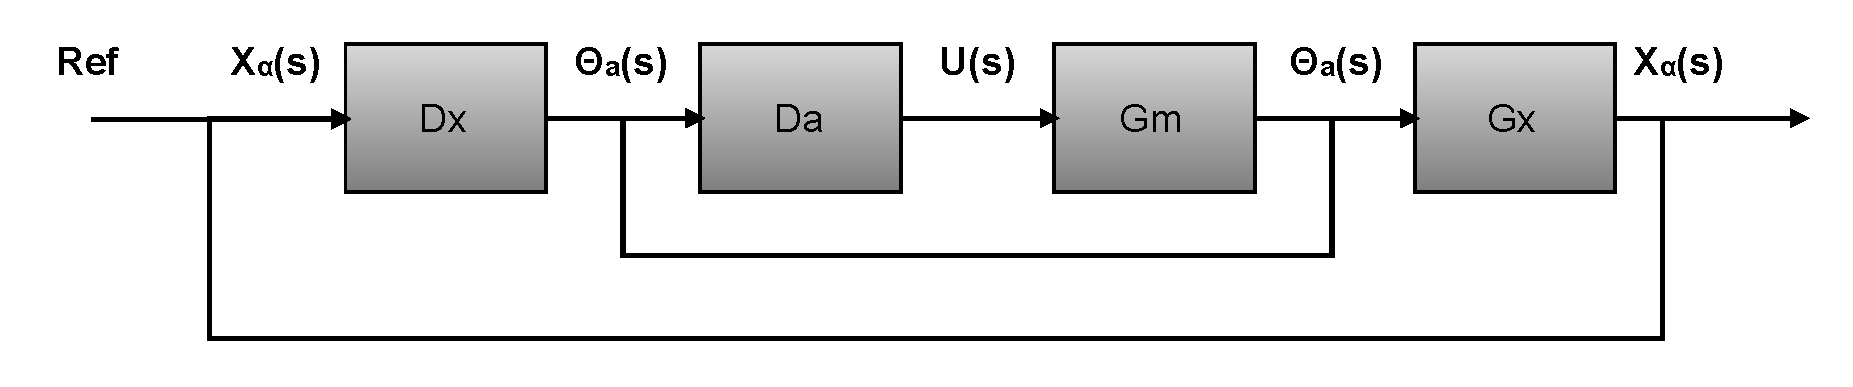
\includegraphics[width=\textwidth]{IPBlock}
\caption{Block diagram of the inverted pendulum system with inner and outer loop controllers.}
\label{fig:IPBlock}
\end{figure}
%
%If the inner loop is faster than the outer loop then it can be assumed to be irrelevant when designing the outer loop controller.

With the redefined transfer function the outer loop will control the transfer function in \autoref{eq:xaTF}. From the root locus in \autoref{fig:locusxa} it can be seen that a zero needs to be added on the real axis in the left half plane in order to move the pole in the right half plane to the stable region. 

\begin{figure}[htbp]
\centering
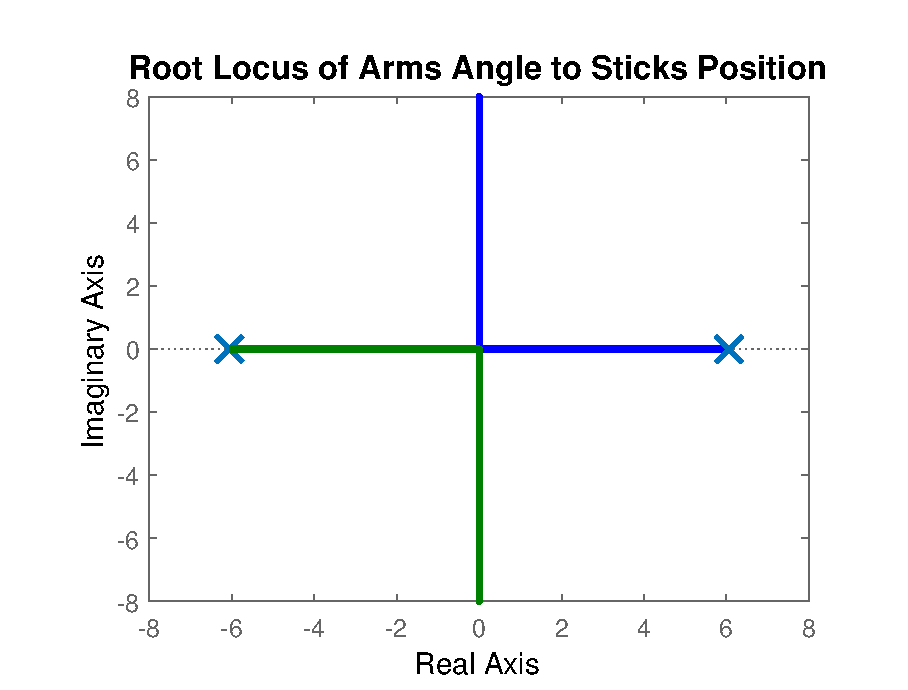
\includegraphics[width=0.7\textwidth]{rlocusRedef}
\caption{Root locus of the transfer function from the angle of the arm to the position of a point on the stick.}
\label{fig:locusxa}
\end{figure}

If the zero is positioned between the two poles both the right most will move towards the zero while the leftmost moves towards infinity; both along the real axis. Positioning the zero close to the origin doesn't allow for the pole to move far into the left half plane. If it's put far to the left of the stable pole the poles will move off the real axis and to the left of the zero with higher gain. This can move them very far into the left half plane before they come back to the real axis which could cause issues for making the inner loop faster than the outer loop. This is because the further away the poles are from origin the higher the natural frequency and a high natural frequency means small settling time. If the poles are off the real axis it'll introduce overshoot which needs to be under 10\% per the specifications. 

Placing the zero close to the leftmost pole would allow for the unstable pole to move further into the left half plane without an overly fast response or any overshoot. 

The zero could theoretically be placed on the pole to cancel it and allow the pole to move further into the left half plane along the real axis. This would be ideal but the true location of the pole of the real system is difficult to find as small variations in measurements of the system could move the pole slightly. 

The zero will initially be placed on the pole as it doesn't change the system drastically whether it's slightly off to either side. The pole is then placed at $-\sqrt{\frac{3g}{2l_s}}$. This can be seen in \autoref{fig:rlocusZeroAdded}.

\begin{figure}[htbp]
\centering
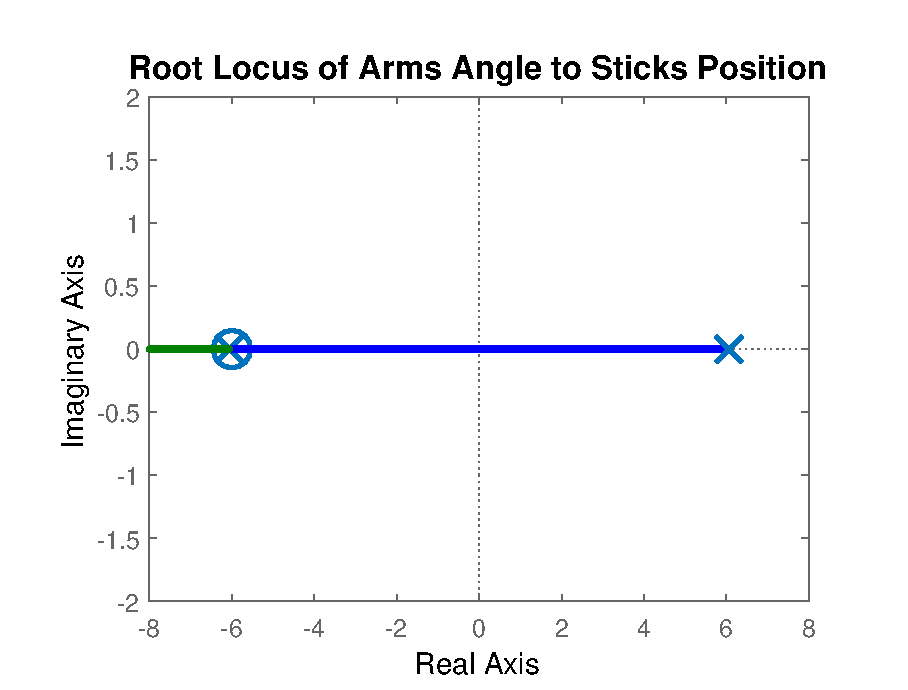
\includegraphics[width=0.7\textwidth]{rlocusZeroAdded}
\caption{Root locus of the outer loop system with a zero cancelling the left pole.}
\label{fig:rlocusZeroAdded}
\end{figure}

The unstable pole can now enter the stable region by selecting a gain large enough. Simply adding a zero to the system will however amplify high frequencies. This can be avoided by adding a pole further into the left half plane. This effectively makes the controller a lead controller. The position of the pole and the gain will determine the settling time and overshoot of the system. The settling time for the outer loop controller should be more than 10 times slower so the assumption, that the inner loop controller is much faster than the outer loop controller, holds true. As the gain increases the two poles move closer to each each other before meeting and moving into the imaginary plane. The gain will be selected to be however much is needed for the poles to meet. The pole can then be selected such that the place where the poles meet will give a settling time 10 times slower than the inner loop.

As the settling time of the inner loop is \textbf{TBD!}, the natural frequency of the outer loop can be approximated by \autoref{eq:outerWn}. 
\begin{subequations} \label{eq:outerWn}
\begin{flalign}
T_{s_{outer}}(2\%) &=-\frac{\ln(0.02)}{\zeta\cdot \omega_n} \\
\omega_n &=-\frac{\ln(0.02)}{\zeta\cdot T_{s_{inner}}\cdot 10} \\
\omega_n &=-\frac{\ln(0.02)}{1\cdot 0.157 \cdot 10} \\
\omega_n &=2.49
\end{flalign}
\end{subequations}

This approximation only holds true for 2nd order systems without zeros which this would only be if the zero placed exactly on the pole removes both which is not the case. The approximation will however still be a good start.
To achieve a natural frequency of 2.49, the lead controller pole needs to be placed so the halfway point between it and the unstable pole is 2.49. This means that the end location of both poles will be in -2.49. The pole location is then found by \autoref{eq:outerLeadPole}.
\begin{subequations} \label{eq:outerLeadPole}
\begin{flalign}
-2.49&=\frac{p_{unstable}+p_{lead}}{2} \\
p_{lead} &=-2.49\cdot 2-\sqrt{\frac{3g}{2l_s}} \\
p_{lead} &=-9.27 
\end{flalign}
\end{subequations}

This can be seen on \autoref{fig:rlocusLead}.
\begin{figure}[htbp]
\centering
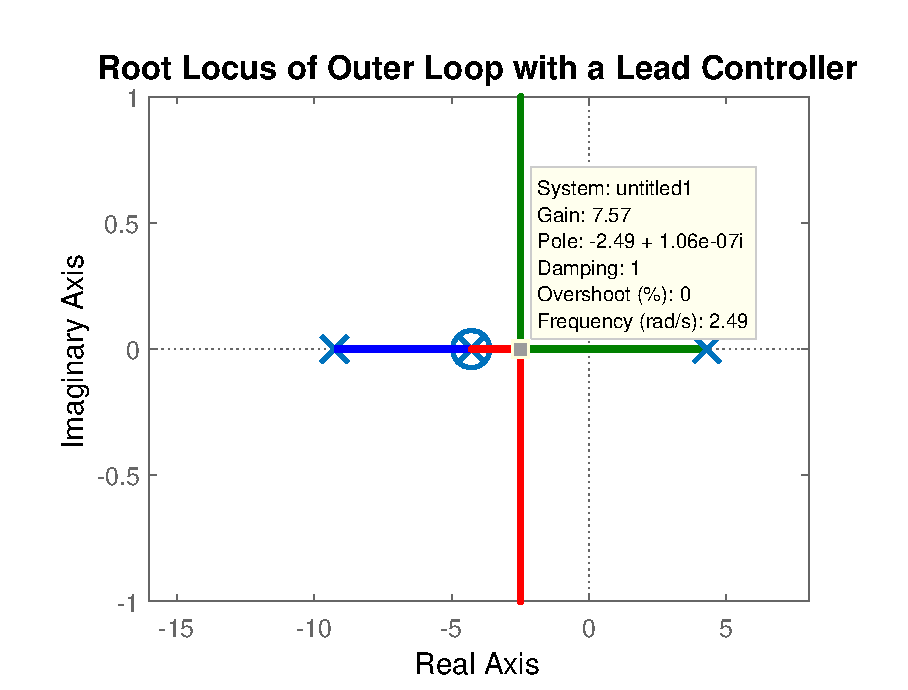
\includegraphics[width=0.6\textwidth]{rlocusOuterLead}
\caption{Root locus of the outer loop with the lead controller.}
\label{fig:rlocusLead}
\end{figure}

To make the two poles meet a gain of 7.57 is needed. This gives a lead controller of \autoref{eq:IPLead}.
\begin{flalign}
D_{x}=7.57\frac{s+\sqrt{\frac{3g}{2l_s}}}{s+9.27}\label{eq:IPLead}
\end{flalign}

The settling time is found by looking at the step response on \autoref{fig:stepOuterLead}.
\begin{figure}[htbp]
\centering
\missingfigure{}
\caption{Step response showing the settling time of the outer loop with a lead controller.}
\label{fig:stepOuterLead}
\end{figure}

The settling time is slower than calculated and this is because the zero and pole at the same location still has an influence on the system. A bit of overshoot can also be added in this system to get a faster rise time but a similar settling time. This is okay as the specifications are only for overshoot of the angle of the stick. It's uncertain how an overshoot when controlling the distance to a point on the stick will affect the angle of the stick. A maximum overshoot for the distance is therefore arbitrarily chosen to be the same as the overshoot for the angle.
To get a settling time of 1.6 seconds a new gain needs to be found to give a faster settling time but no more than 10\% overshoot. If it's not possible without more than 10\% overshoot the controller pole has to be moved further to the left

The lead controller then becomes \autoref{eq:outerLeadController}.
\begin{flalign}
D_x=8.85\frac{s+\sqrt{\frac{3g}{2l_s}}}{s+9.27}\label{eq:outerLeadController}
\end{flalign}

This controller gives a fast rise time, a settling time of 1.6 seconds and overshoot of less than 10\%. This can be seen on the step response on \autoref{fig:stepOuterLeadOvershoot}.
\begin{figure}[htbp]
\centering
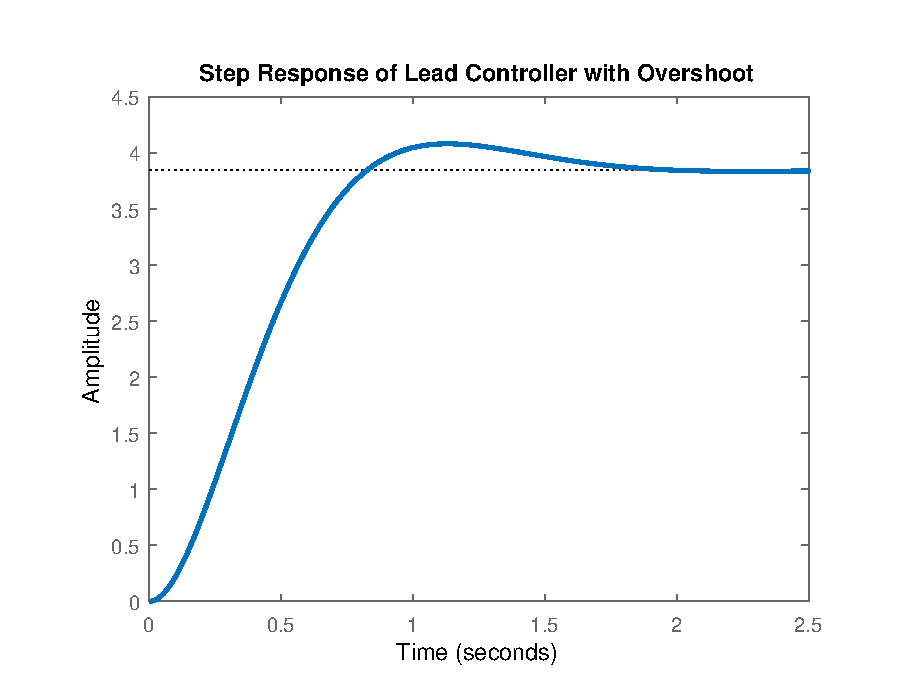
\includegraphics[width=0.7\textwidth]{stepOuterOvershoot}
\caption{Step response of the outer loop with the lead controller that gives less than 10\% of overshoot.}
\label{fig:stepOuterLeadOvershoot}
\end{figure}

\todo[inline,author=Jacob]{All these numbers are calculated with inner loop settling time of 0.157 and ls=0.8 meters.}

%Selecting the gain too large will however move the other pole further into the left half plane making it more difficult to make the inner loop system faster than the outer loop. As both the zero placement and gain needs to be adjusted later in conjunction with the inner loop controller, the gain will be set to 1 as this puts the unstable pole in the left half plane without the other pole moving too far away as seen on the pole-zero plot on \autoref{fig:pzouterloop}.
%\begin{figure}[htbp]
%\centering
%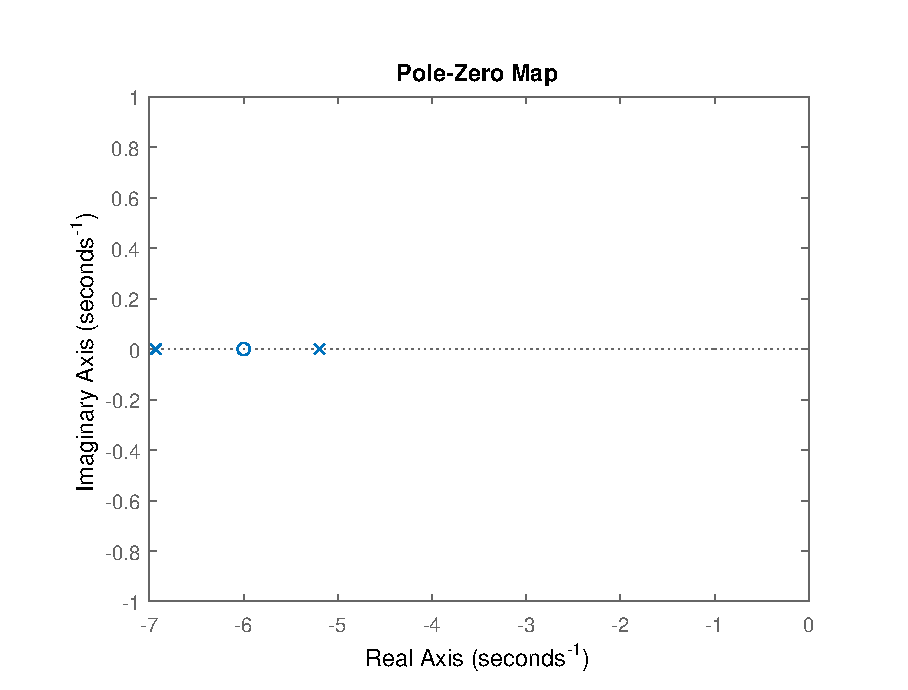
\includegraphics[width=0.7\textwidth]{pzouterloop}
%\caption{Pole-zero plot of the system with the outer loop controller in feedback.}
%\label{fig:pzouterloop}
%\end{figure}







%\todo[inline,author=Jacob]{For the rest of this section: Use root locus to design Dx controller (Maybe parts of next section can be used here), then design Dm controller while keeping in mind it should be faster than Dx. I'd like for the angle of the stick to somehow be shown as a disturbance in the system and relate the redefinition to feedforward control for better disturbance rejection if possible. Tune parameters in the end as inner loop will have an effect on outer loop.}

%\section{Controller with a 2nd right half plane pole added}
%\todo[author=Jacob, inline]{A lot of this only applies for 2nd order system which this is not. I already wrote it without considering that so this section might have to be deleted but I'm leaving it for now. 2 zeros in 0 is also a massive pain in the ass.}
%A different control method will be attempted in this section where the model won't be redefined but rather a 2nd pole will be added to the right half plane in an attempt to circumvent the zeros in 0.
%
%This controller adds a zero and a pole to the system and thus have three variables that needs to be chosen: The gain and the locations of the zero and the pole. The pole has to be located somewhere in the right half plane and the zero in the left. Their exact locations influence the root locus of the system.
%
%To make the system as stable as possible a fast rise time and low overshoot is desirable. From the specifications the overshoot is set as maximum 10\% with no requirements for the rise time. The damping ratio, $\zeta$, can be found from the overshoot percentage, $M_p$, by \autoref{eq:IPOvershoot}.
%\begin{subequations}
%\begin{flalign}
%& M_p=100\exp^{\frac{-\pi\zeta}{\sqrt{1-\zeta^2}}}<10\%  \\
%& \zeta = \sqrt{\frac{\left(\ln{\frac{M_p}{100}}\right)^2}{\pi^2+\left(\ln{\frac{M_p}{100}}\right)^2}}  \\
%& \zeta > \sqrt{\frac{\left(\ln{\frac{10\%}{100}}\right)^2}{\pi^2+\left(\ln{\frac{10\%}{100}}\right)^2}} = 0.59 \label{eq:IPOvershoot}
%\end{flalign}
%\end{subequations}
%
%The damping ratio then has to be larger than 0.59 in order to have a overshoot of less than 10\% as specified. The rise time, $t_r$, is approximated by \autoref{eq:IPRisetime}.
%\begin{flalign}\label{eq:IPRisetime}
%& t_r =\frac{2.2}{\zeta\omega_n} 
%\end{flalign}
%
%In order to get as fast a rise time as possible the natural frequency and damping ratio both needs to be maximized. The natural frequency can be found on the root locus by the length from the poles to the origin. The damping ratio is found by the angle from the imaginary axis to the poles. As both $\zeta$ and $\omega_n$ are dependent on the pole locations it's possible that the fastest response time comes with a damping ratio below 0.59. The goal of this controller is to minimize \autoref{eq:IPRisetime} but maintaining a damping ratio above 0.59.
%
%The location of the pole, and zero and the gain can thus be decided in order to achieve final pole locations with as far away from the origin as possible while having an angle to the imaginary axis that corresponds to $\zeta=0.59$.

%For the inverted pendulum it's also worth to consider a controller that keeps the arm at zero radians as well as it has a much harder time controlling the arm when out of the upright position. Therefore two controllers will be made: A single-input single-output (SISO) controller that only controls the angle of the stick and a single-input multiple-output (SIMO) controller that controls both the angle of the stick and the arm. 
%\todo[inline,author=Jacob]{If time allows. Otherwise just SISO.}

%\section{Single input single output controller for the inverted pendulum}
%For the SISO controller at least a zero or pole must be introduced along with the P-controller in the system in order to move the pole in the right half plane to the left half plane. For the pole in the right half plane to cross into the left half plane a pole must be added either in 0 to cancel the zero or in the right half plane forcing both off the real axis and allowing them to circumvent the zero in 0 and enter the stable region.


\chapter{Design of the Rocket and Gimbal Controller}
The following chapter describes the design of the rocket and its control system. The main objective is not to design the rocket, but to implement at control system that can stabilize it during launch and flight. 

\section{Rocket Design}
For the purpose of studying the problem of the rocket control, a model rocket was designed and built. Since mechanical design is out of this work's scope, the engineering of this rocket will not be explained, but the design CAD files will be available on the GitHub repository.\todo{Add the github link later.}
This design consists of 2 sections, that will be called "stages".


\textbf{First stage: propulsion}
\begin{itemize}[noitemsep]
	\item {A thruster / Solid Rocket Booster (SRB)}
	\item {A thrust vectoring mechanism, also known as gimbal, with two degrees of freedom}
	\item {Two servo motors for actuating the gimbal}
\end{itemize}

\textbf{Interstage:}
\begin{itemize}[noitemsep]
	\item {An empty fairing separating the propulsion stage from the electronics}
\end{itemize}
\textbf{Upper stage: control}
\begin{itemize}[noitemsep]
	\item A frame to contain the electronics.
	\item A PCB with a micro-controller.
	\item A plastic separator with anti-vibration bearings.
	\item On this separator is placed a gyroscope: the attitude sensor.
	\item A nose fairing.
\end{itemize}

\subsubsection*{Choice of thrusters for the rocket}
A thruster is a central component in all types of rocket. In the project the thruster will be chosen based on availability and lift force. The maximum weight of the rocket can not exceed 300 grams and the thruster should be able to lift this. The average thrust of the thruster should be have at least a average thrust of 3 Newton. The choice is limited to the thrusters which can be acquired within the European regulations. Through superficial research it is found that Klima 18 mm rocket motors is legal in all of Europe, and will be chosen for the thruster. The chosen thruster is the version D3-P with the specifications cf. table \ref{ThrusterValue}.

\begin{table}[]
\centering
\begin{tabular}{lll}
\hline
Parameter      & Value         & Unit \\ \hline
Total impulse  & 17,4          & [N]  \\
Average thrust & $\approx$ 3   & [N]  \\
Maximum thrust & $\approx$ 9 & [N]  \\
Burn duration  & $\approx$ 5,5 & [s]  \\
Weight         & 0,105         & [kg] \\
Length         & 0,07          & [m] 
\end{tabular}
\caption{DP-3 thruster specifications}
\label{ThrusterValue}
\end{table}
                
%http://www.modelrockets.co.uk/shop/klima-model-rocket-motors/d3-six-pack-18mm-rocket-glider-motor-p-3311.html

\subsubsection*{Physical Parameters of the Rocket}
The important factors for controlling the rocket is the physical parameters. These will effect how the rocket would transfer a input to its output. We can not control the force of the thruster, and this can will therefore not be a part of the important   		
\begin{table}[htbp]
	\centering
	\begin{tabular}{llll}
	\hline
	Piece & Parameter & Value & Unit \\ \hline
	Rocket$_{overall}$ & Height & 297 & {[}mm{]} \\
	Rocket$_{overall}$ & Weight & 0,28 & {[}kg{]} \\
	Interstage & Diameter & 67 & {[}mm{]} \\
	Thrust vectoring system & Max. angle & ? & {[}rad{]}\\
	Thrust vectoring system & Response time & ? & {[}rad/s{]}
	\end{tabular}
\caption{Parameters of the rocket.}
\label{Rocket_measurements}
\end{table}
\todo{Input the rest of the parameters.}

\startexplain
\explain{Rocket$_{overall}$ is the total weight of the system, including thruster, electronics, and rocket structure.}{}
\stopexplain


\subsection{Choice of Sensors for the Rocket}  \label{sec:Rocket_sensor_choice}

The following sections describes the sensors chosen for implementation in the rocket. It is chosen that the microcontroller unit, from here on named MCU, used in the system will be a Arduino Nano. The Nano is chosen based on its low weight (7 grams) and small size (18 x 45 mm) which will be an advantage when fitting it in the rocket.    

As described in section \ref{sec:PRocketAnalysis} the rocket can be a system with instability problems. In the inverted pendulum these instabilities is detected trough sampling sensors and corrected trough a DC motor control system. The same parameters is considered when controlling the rocket. A form of sensor is needed to detect the orientation and position of the rocket, and a control system is needed to counteract changes from the initial trajectory.

Choosing sensors for the rocket will be weighted based on following parameters:

\begin{itemize}[noitemsep]
\item Compatibility.
\item Power consumption.
\item Availability. 
\item Physical dimensions and weight.
\end{itemize}

Needed is a sensor for measuring:
\begin{itemize}[noitemsep]
\item Orientation.
\item Acceleration.
\item Temperature and barometric pressure.
\end{itemize}

Determining the altitude, orientation and acceleration of the rocket can be done with different types of sensor. Two types of sensors can be considered when involving rockets; reference sensors and inertial sensors. Reference sensors have a external reference to measure from where inertial sensors measures changes in it physical state from its inertial state. Commonly used sensors and applications is listed, these determined from different types of rocket applications:

\begin{itemize}[noitemsep]
\item Gyroscope
\item Accelerometer
\item Global Positioning System (GPS)
\item Magnetometer
\item Barometric pressure sensor
\item Infrared camera
\item Solar panels
\end{itemize}

Some sensors can easily be declined from the choice. This is mainly because there application is most commonly with rocket going to higher altitudes or even in-orbit around earth, which is not the interest in this project. For example is the infrared camera implemented in some satellites and rocket to determine the position of the earth relative to the satellite. This will not be implemented in the rocket, because the altitude of the rocket is too low. Equally is solar panels implemented mostly in satellites, because the time span for change is lower than when launching and correcting a rocket.
Sensors considered in the project is gyroscopes, accelerometers, magnetometer/compass, GPS, barometric sensor. 

GPS is a relatively common used component in flying systems. It is implemented in many quad-copters, where the goal is to hold a position based on GPS. In the rocket it can be used to determined velocity, deviations from trajectory, and altitude. Precise and fast GPS units have a high cost and higher power consumption than alternatives. It is therefore decided that GPS will not be included as a component of choice.    

An accelerometer measures acceleration in one to three axis(x,y,z). The reference for measuring is the gravitational force. A single axis accelerometer can measure the acceleration in the direction it is orientated. And can for example be used to determine the velocity upwards flying rocket. This can as well be used to determine a travelled distance based on knowing the acceleration and time. In the case of flying a rocket a three-axis accelerometer would be the implemented, when considering that the rocket can move both lateral and vertical in its position.  


A gyroscope is on the other hand measuring the angular velocity changes in three dimensions. The difference between the accelerometer and gyroscope is that the gyroscope is capable of measuring the rate of rotation around an axis. It does not rely on a fixed reference and is commonly used in applications like drones and other flying objects. In the rocket it can be used to determine the orientation and rotation of the rocket based on measuring the rate of changes in any direction.  


Combining these gives a Inertial Measurement Unit(IMU), which is commonly used in model planes and quad-copters. The application of this is to obtain the objects position through measuring velocity, orientation, rotation with the gyroscope and accelerometer. Both types of components are dependent of temperature and barometric pressure, so often an IMU includes multiple types of additional sensors for calibration purposes. A choice is made to use an IMU, given that its application in similar types of flying systems verifies that it is suitable for a rocket.    	  
Some performance factors must be considered when choosing a IMU. For example is the g-force range of the IMU important. If the maximum ratings is lower than the acceleration of the rocket, then the sensor would not be able to give sufficient data at maximum acceleration. As well is the sensitivity of the accelerometer important. The rocket is a system with a high amplitude g-force when launching, and therefore a accelerometer with low sensitivity is preferable.

\subsubsection{Inertial Measurement Unit - GY-87}
GY-87\cite{web:GY80} is an IMU made available for use. It includes an MPU6050, which combines a 3-axis accelerometer and a 3-axis gyroscope, a BMP180 thermometer/barometer, and a HMC5883 3-axis magnetometer. It is chosen based on its combination of components, low power consumption of $\approx$ 6,5 mA in measurement mode. It is designed so it can be implemented with the Arduino Nano through I2C communication. 
I2C is a two wire protocol which is working trough serial communication. I2C is based on having two wires between the Arduino and the GY-87. The one wire SCL is the serial clock, and the other wire SDA is the data wire. All components on the GY-87 are convenient to implement with the Arduino. Further analysis is described cf. section \textbf{[ref]} \todo{Ref to to implementation part when it is done.}



\section{Rocket Controller Design}\label{sec:RocketControllerDesign}
The following sections explains the design procedure behind fitting the transfer function and dynamics of the rocket with a feedback controller. The controllers goal is to change the orientation of the thruster trough regulating the thrust vectoring system.    

\graphicspath{{figures/Design/IPController/}}
\chapter{Design of the rocket Controller}\label{sec:IPController}
The goal of the controller is to balance the rocket body in an upright position. 

As seen in the modeling of the rocket, the system presents poles and zeros in the origin of the pole-zero plot. The system is unstable and goes to infinity on the imaginary axis. To solve this problem a zero could be added at a higher frenquency to attract the poles.

				% Figure of original tf
\begin{figure}[htbp]
	\centering
	
		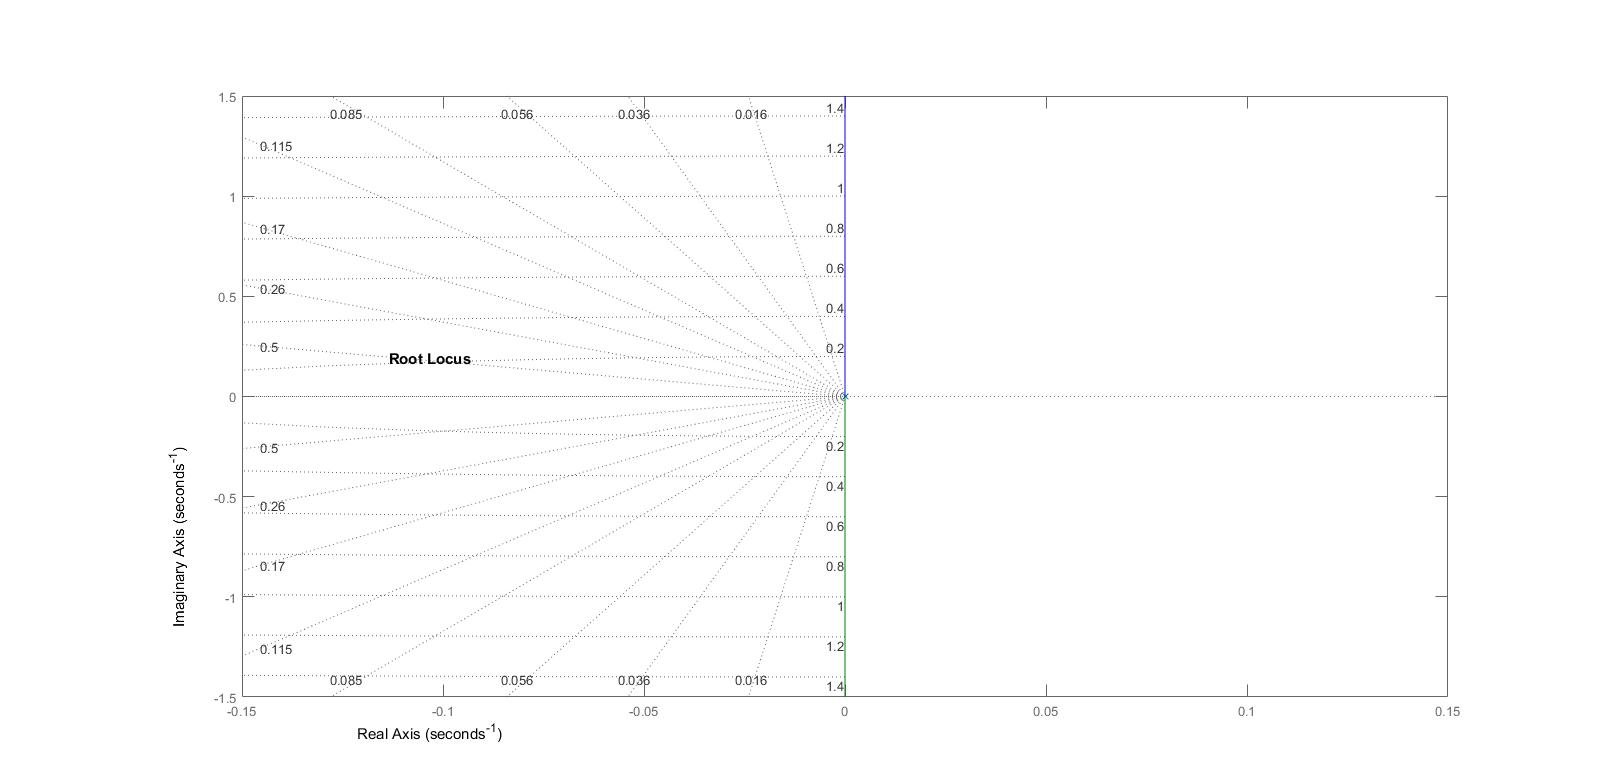
\includegraphics[width=\textwidth]{figures/Rocket/design/initial_transfer_function}
		\caption{Root locus of the initial rocket angle transfer function.}
		\label{fig:Rinitialtf}
	
\end{figure}

However the real system is influenced by the servomotors. The transfer function of the servomotors adds a pole, resulting in an unstable system moving towards infinity on the imaginary axis. 
				
				% Figure of tf + servo
\begin{figure}[htbp]
	\centering
		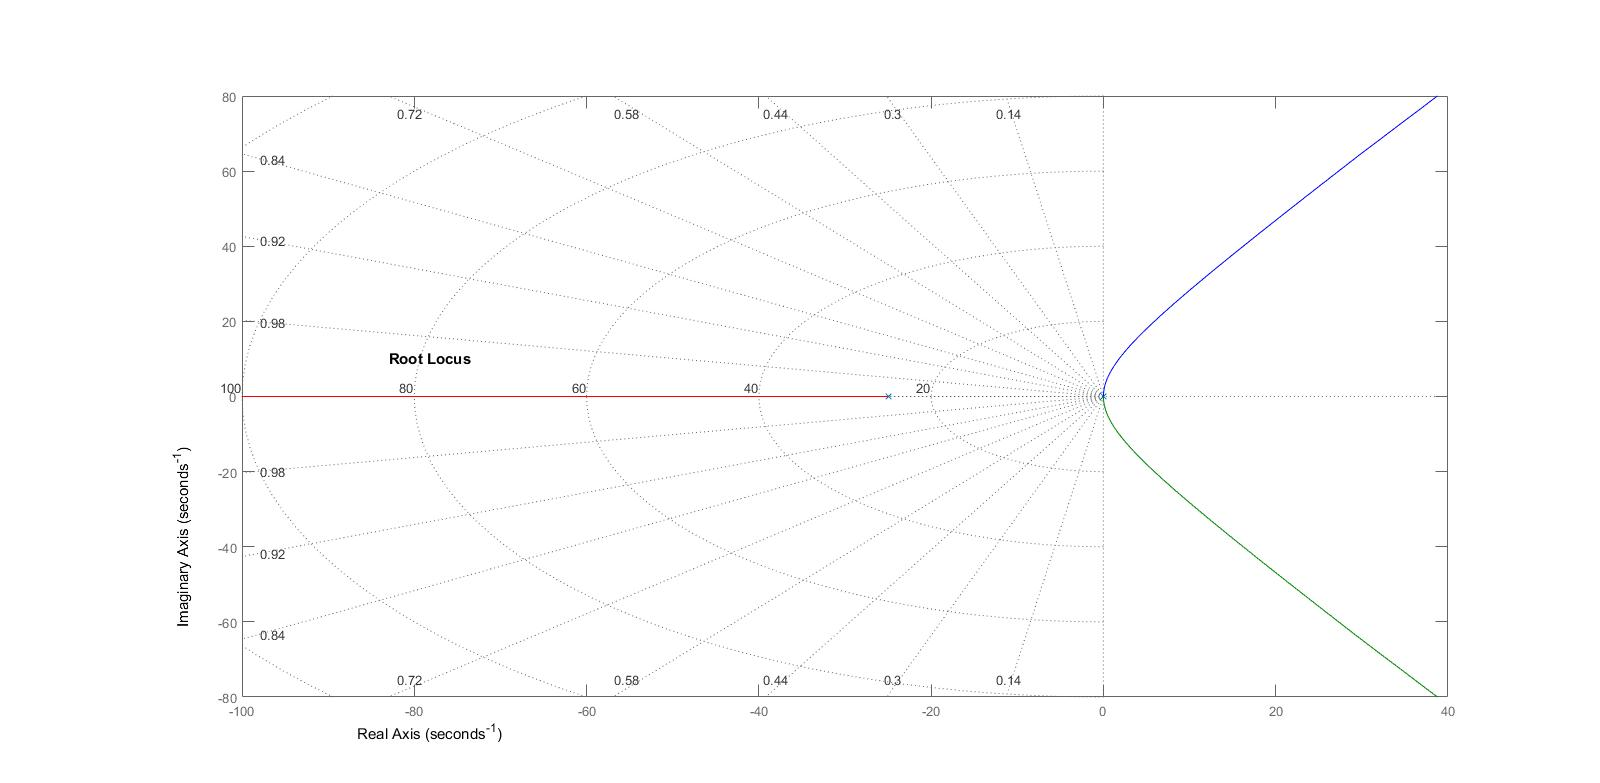
\includegraphics[width=\textwidth]{figures/Rocket/design/tf_with_servo}
		\caption{System with the servomotors.}
		\label{fig:SystemServo}
\end{figure}

To direct the root locus to a stable state, a controller C1, adding a zero and a pole on the left side, is implemented. The zero of the controller is chosen to be near the system in order to attract the poles. The pole of the controller is set at high frequency to not temper with the system. 

				% Figure of tf + servo + C1, and zoom of tf + servo + C1
\begin{figure}[htbp]
	\centering
	\begin{subfigure}{0.45\textwidth}
		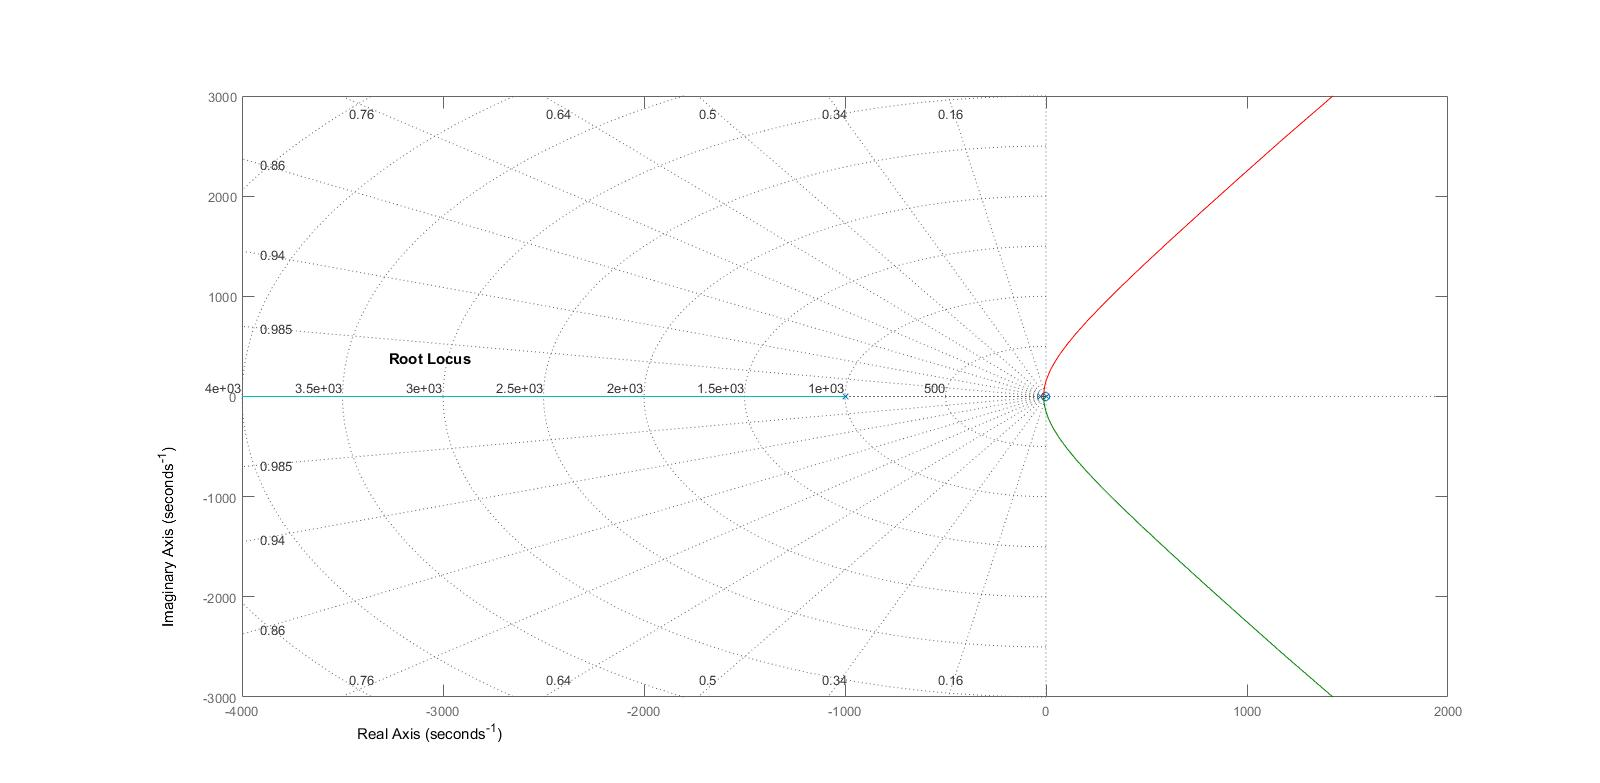
\includegraphics[width=\textwidth]{figures/Rocket/design/tf_with_controller_1C_1}
		\caption{Total view of the poles and zeros.}
		\label{fig:SystemC1}
	\end{subfigure}
	\begin{subfigure}{0.45\textwidth}
		\centering
		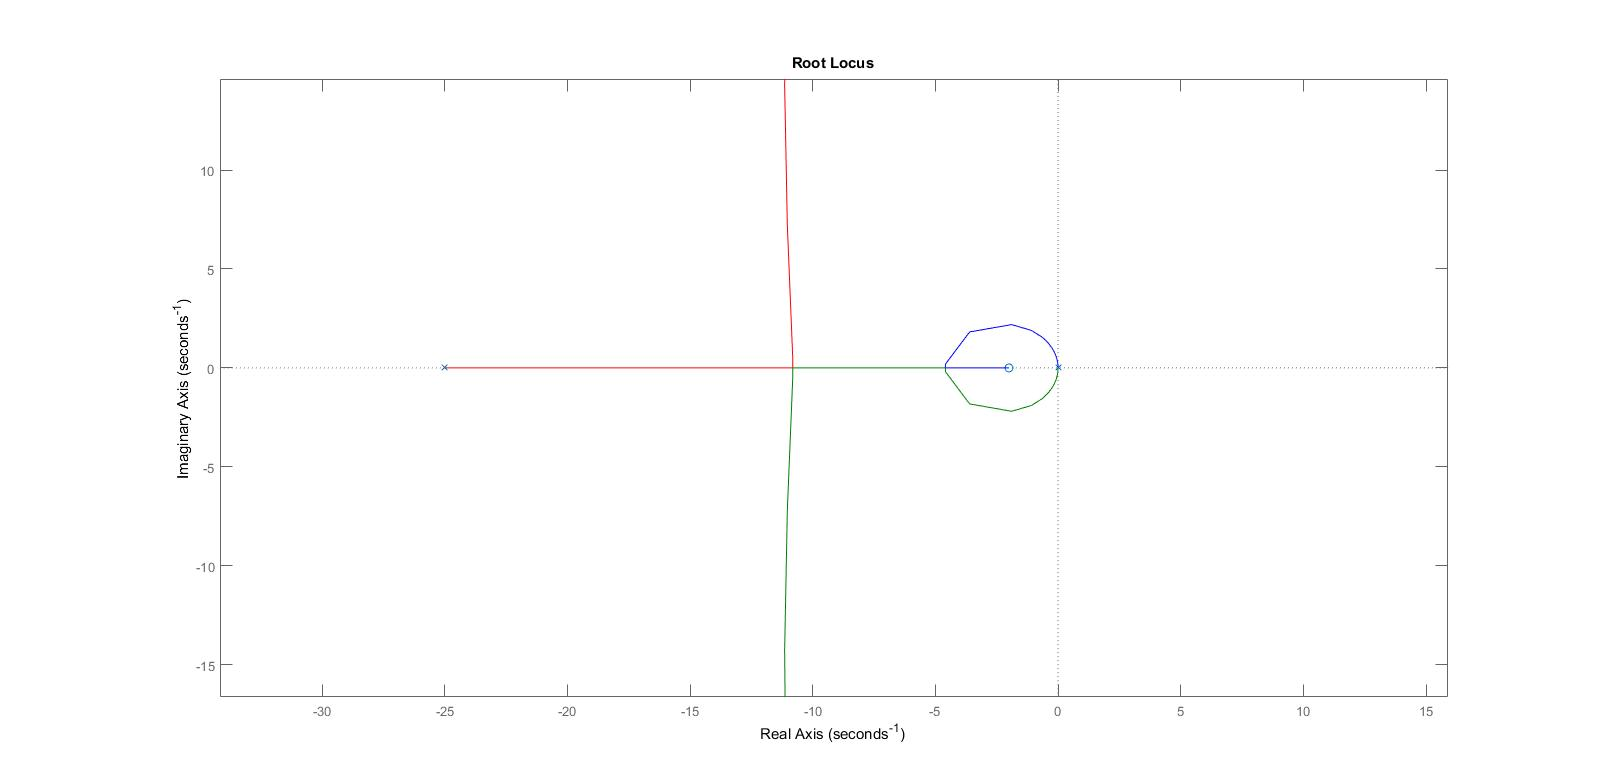
\includegraphics[width=\textwidth]{figures/Rocket/design/tf_with_C1_zoom}
		\caption{Focus on low frequencies.}
		\label{fig:SystemC1zoom}
	\end{subfigure}
	\caption{Root locus of the system with C1 implemented.}
\end{figure}

Another controller C2 is needed to attract the two poles going to infinity along the imaginary axis. The pole and zeros of C2 are set at higher frequencies than the first controller C1. 

				% Figure of final tf with controllers 
\begin{figure}[htbp]
	\centering
	
		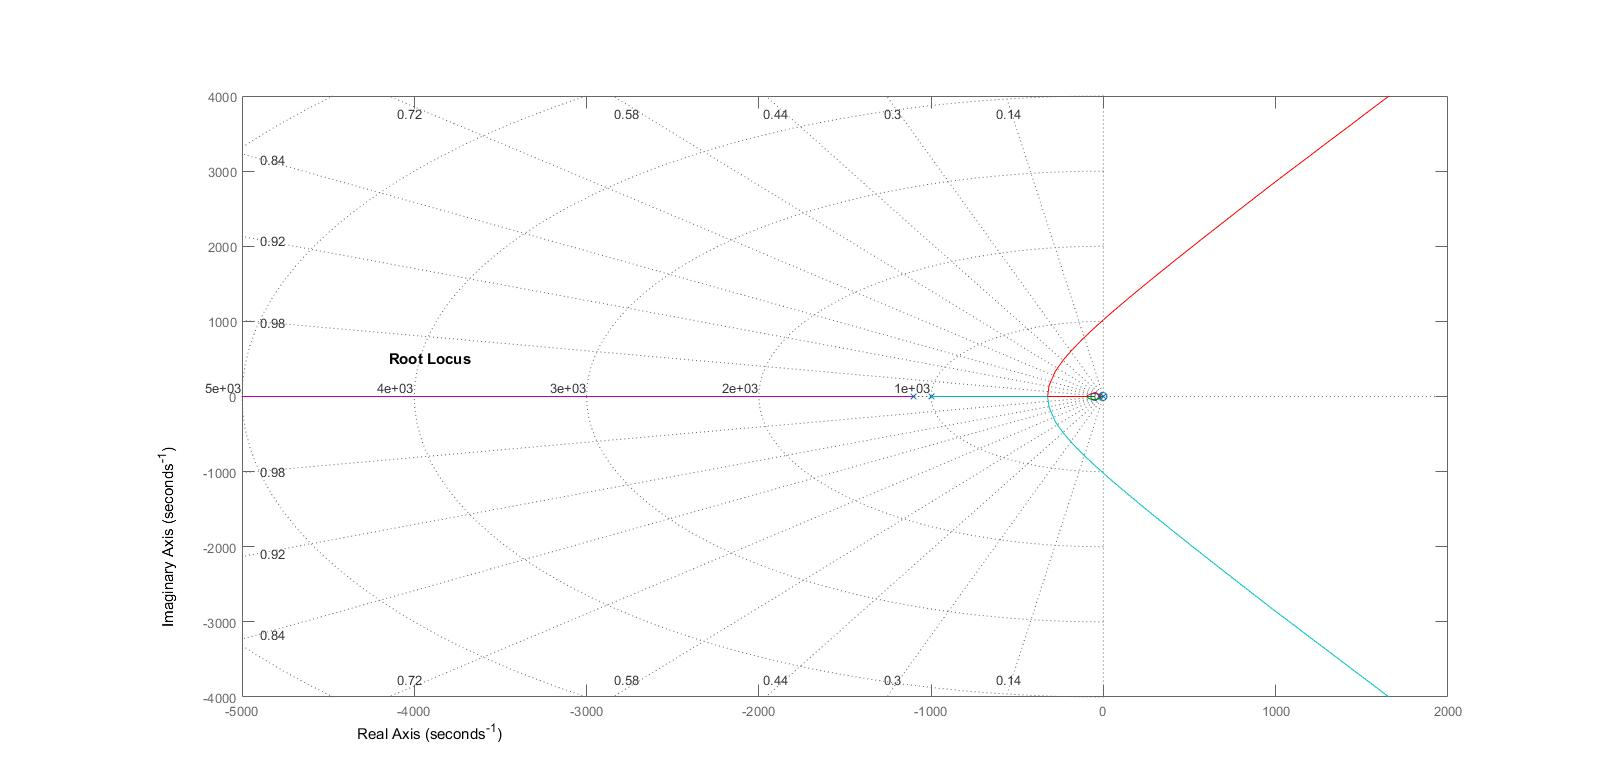
\includegraphics[width=\textwidth]{figures/Rocket/design/tf_with_controller_1}
		\caption{Root locus of the rocket transfer function.}
		\label{fig:SystemC1C2}
		
\end{figure}

The rocket requires a fast settling time and rise time in order to act as soon as possible and control the rocket's stability. Lead compensaters enable the modulation of the rise time, but impact the overshoot. The overshoot is considered as an inferrior error, being in part countered by the play of the gimbal system. 

To improve the setling time, the gain is set at $2.15 * 10^3$ \si{\dB}. This value is chosen by observing the root locus and the gain of a set point as shown on \autoref{fig:SystemC1C2Zoom}.

				% Figure of chosen point, and of final tf with 2.15*10^3
\begin{figure}[htbp]
	\centering
	\begin{subfigure}{0.45\textwidth}
		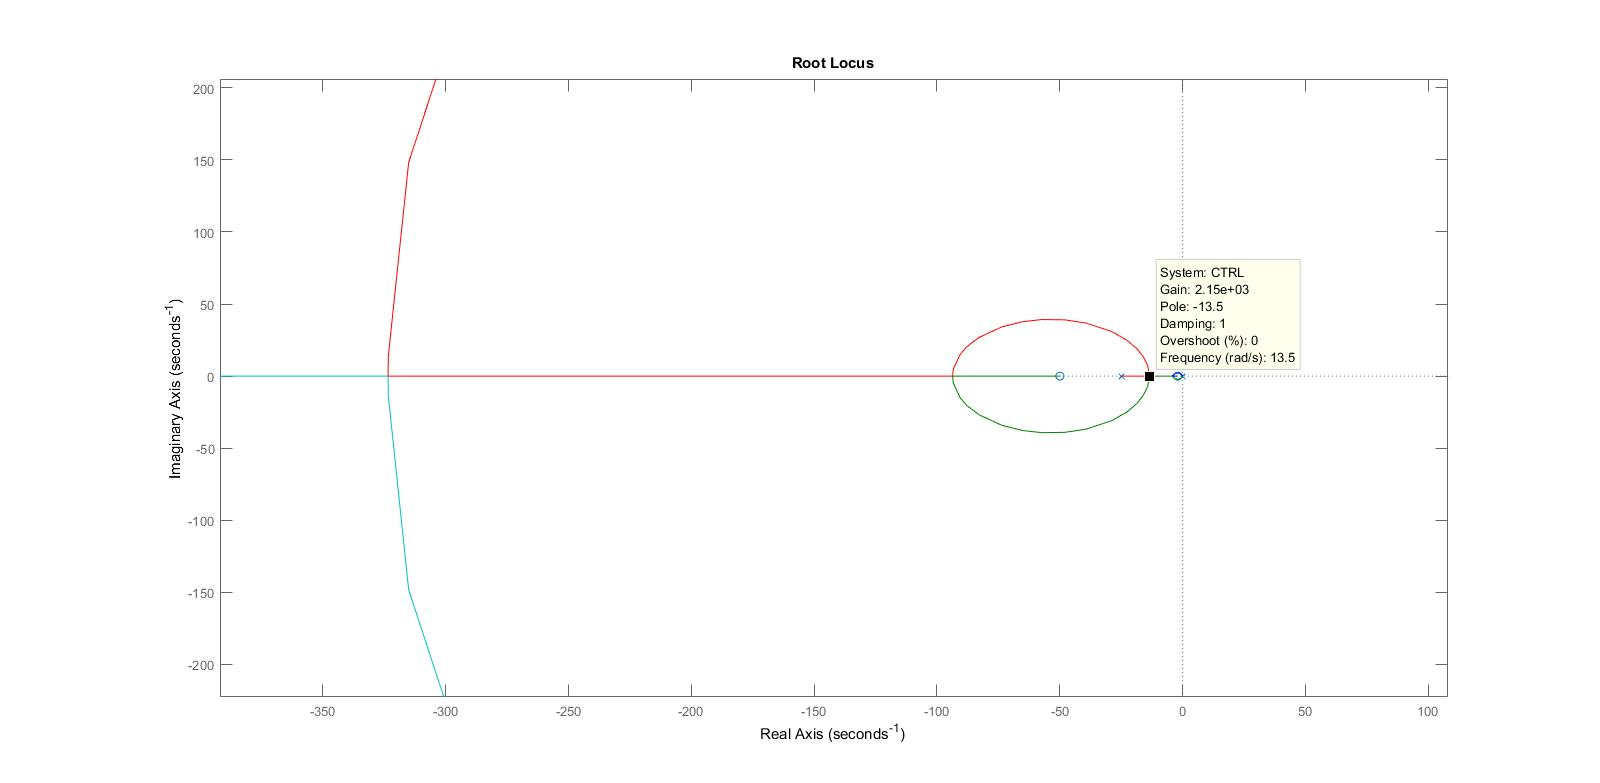
\includegraphics[width=\textwidth]{figures/Rocket/design/tf_with_controller_1_zoom}
		\caption{Set point at the start of the circle.}
		\label{fig:SystemC1C2Zoom}
	\end{subfigure}
	\begin{subfigure}{0.45\textwidth}
		\centering
		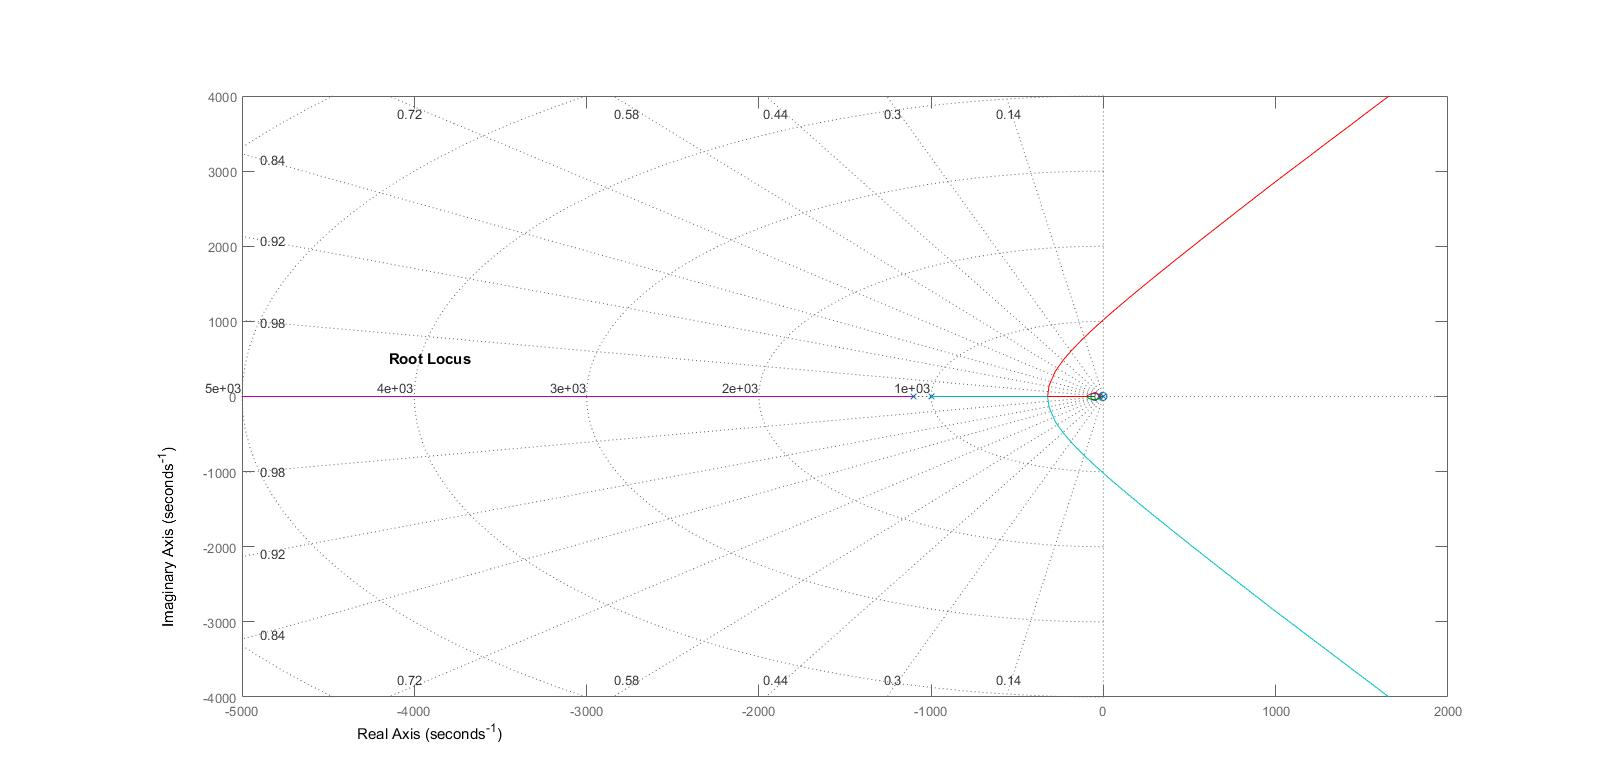
\includegraphics[width=\textwidth]{figures/Rocket/design/tf_with_controller_215}
		\caption{Additional gain of $2.15*10^3$ \si{\dB}.}
		\label{fig:SystemGain215}
	\end{subfigure}
	\caption{Root locus of the rocket transfer function with additional gain of respectively $1$ and $2.15*10^3$ \si{\dB}.}
\end{figure}


The servomotors can have a faster rising time according to the step response of the servomotors, as shown in \autoref{tab:TableStepr}. The gain is then doubled to improve the rise time and setling time. The new adjusted transfer function is observed on \autoref{fig:FinalRocketTf} and \autoref{fig:FinalRocketTfZoom}.

\begin{table}[htbp]
	\centering
	\caption{Simulated step responses.}
	\label{TableStepr}
	\begin{tabular}{llll}
		Transfer function & Rise time{(}s{)} & Setling time{(}s{)} & Overshoot{(}percentage{)} \\ \hline  \rowcolor{lightGrey}
		Servomotors     & 0.0589 & 0.0782 & 0\\  
		Gain of $2.15*10^3$     & 0.1669 & 1.2075 & 14.5609  \\  
		\rowcolor{lightGrey}           
		Gain of $5*10^3$     & 0.0854 & 0.7845 & 12.0162      \\     
	\end{tabular}
\end{table}

				% Figure of final tf with 5*10^3
\begin{figure}[htbp]
	\centering
	\begin{subfigure}{0.45\textwidth}
		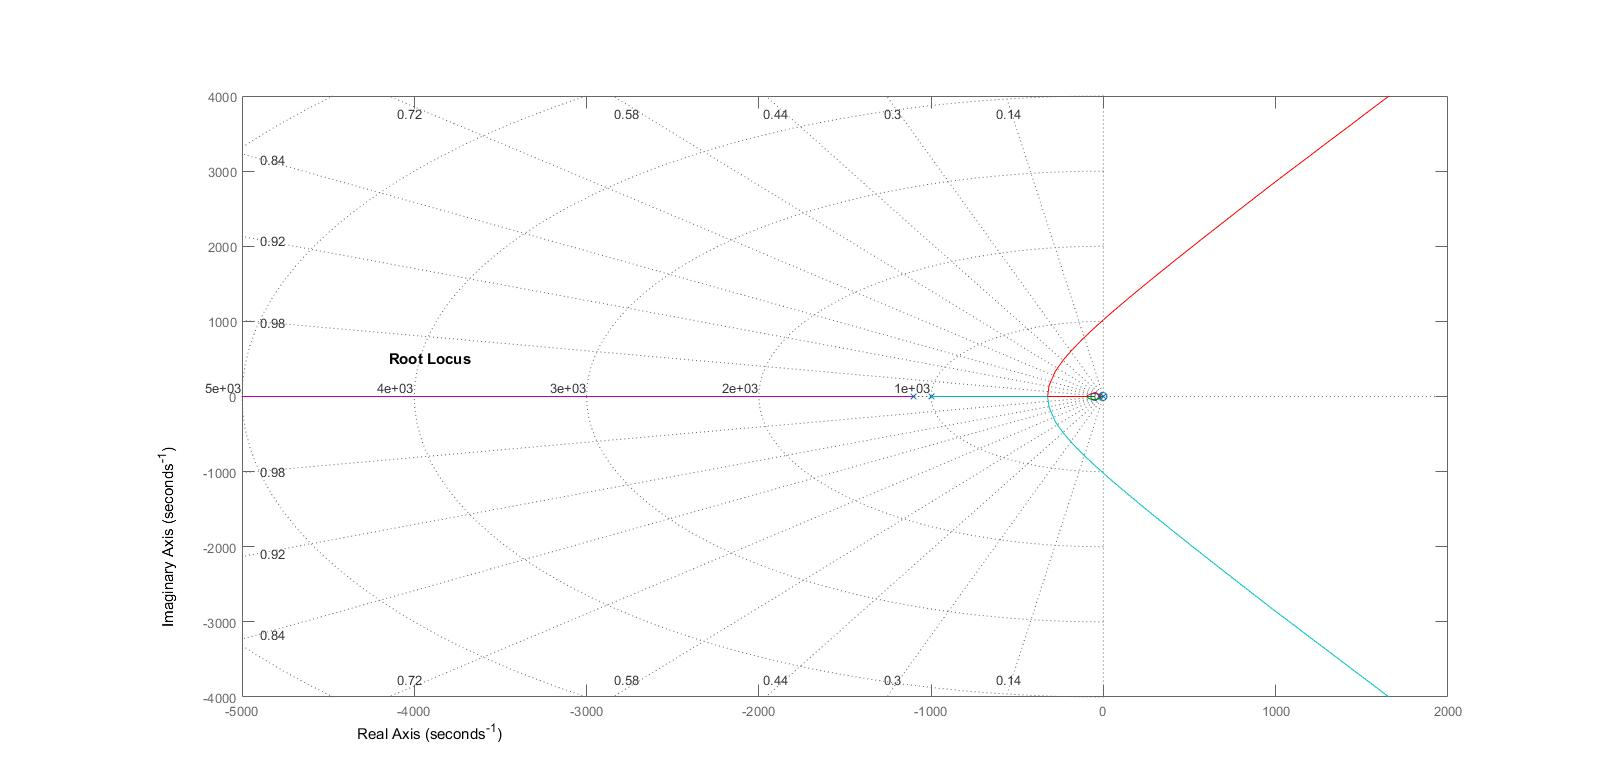
\includegraphics[width=\textwidth]{figures/Rocket/design/tf_with_controller_5}
		\caption{Root locus of the rocket transfer function with an additional gain of $5 * 10^3$ \si{\dB}.}
		\label{fig:FinalRocketTf}
	\end{subfigure}
	\begin{subfigure}{0.45\textwidth}
		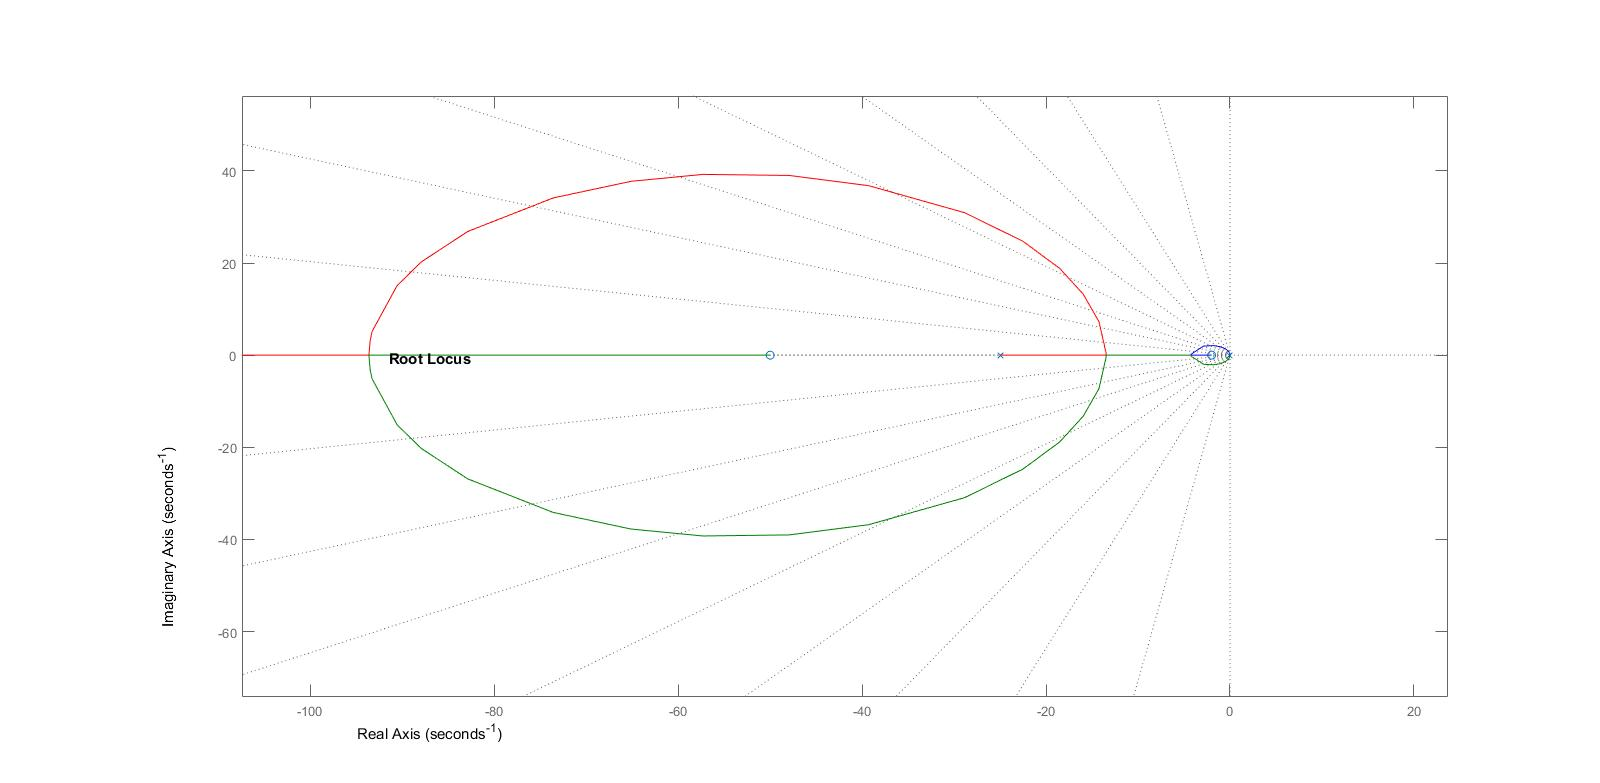
\includegraphics[width=\textwidth]{figures/Rocket/design/tf_with_controller_5_zoom}
		\caption{Focus on lower frequencies.}
		\label{fig:FinalRocketTfZoom}
	\end{subfigure}
	\caption{Root locus of the rocket transfer function with additional gain of $5*10^3$ \si{\dB}.}	
\end{figure}


The frequency correponds to a complete rotation of the servomotors. At low frequencies a delay is observed on \autoref{fig:BodeplotFinalTf}. However the system functions at low speed. This implies that the delay has a tempered effect on the system. Higher frequencies are not physicaly possible and do not need to be compensated.

				% Figure of final tf bodepoint
\begin{figure}[htbp]
	\centering
		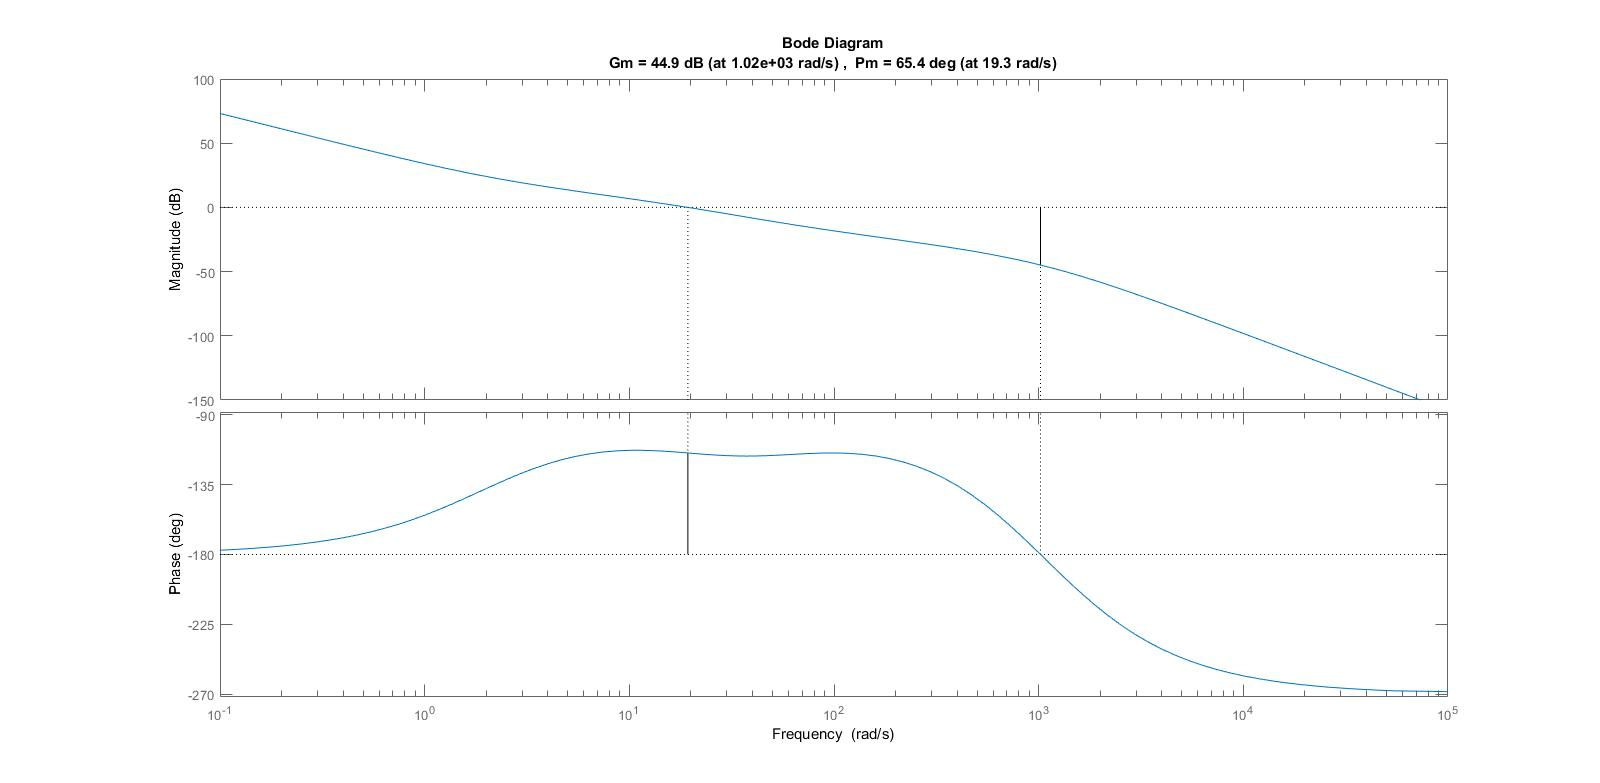
\includegraphics[width=\textwidth]{figures/Rocket/design/bodeplot}
		\caption{Bodeplot of the rocket transfer function.}
		\label{fig:BodeplotFinalTf}
\end{figure}

The controlled rocket transfer function is shown on equation \autoref{eq:RocketTfEqu} and figure \autoref{fig:FinalChart}.

\begin{equation}    \label{RocketTfEqu}
R = 5 \cdot 10^3 \cdot \frac{s + 2}{s + 1000} \cdot \frac{s + 50}{s + 1100} \cdot \frac{1}{s \cdot \uptau + 1} \cdot \frac{F_t \cdot L_{Cg} \cdot \frac{1}{M_r \cdot L_{Es}^2}}{s^2}  
\end{equation}

\begin{figure}[htbp]
	\centering
	
	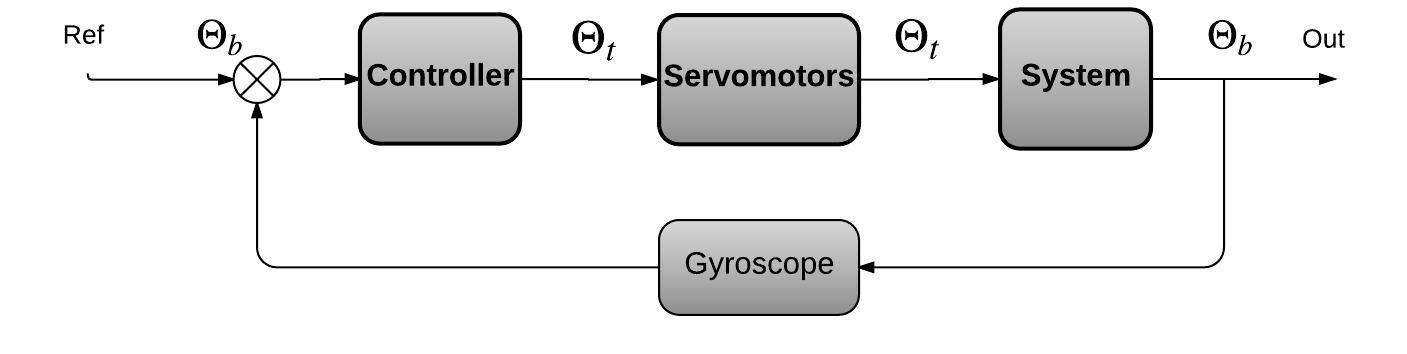
\includegraphics[width=\textwidth]{figures/Rocket/design/final_chart}
	\caption{Rocket transfer function.}
	\label{fig:FinalChart}
	
\end{figure}

\subsection{Design of Thrust Vectoring System}
\todo{Raphael task describe gimbal. - Mathias}

  

%\graphicspath{{figures/Design/IPController/}}
\chapter{Design of the rocket Controller}\label{sec:IPController}
The goal of the controller is to balance the rocket body in an upright position. 

As seen in the modeling of the rocket, the system presents poles and zeros in the origin of the pole-zero plot. The system is unstable and goes to infinity on the imaginary axis. To solve this problem a zero could be added at a higher frenquency to attract the poles.

				% Figure of original tf
\begin{figure}[htbp]
	\centering
	
		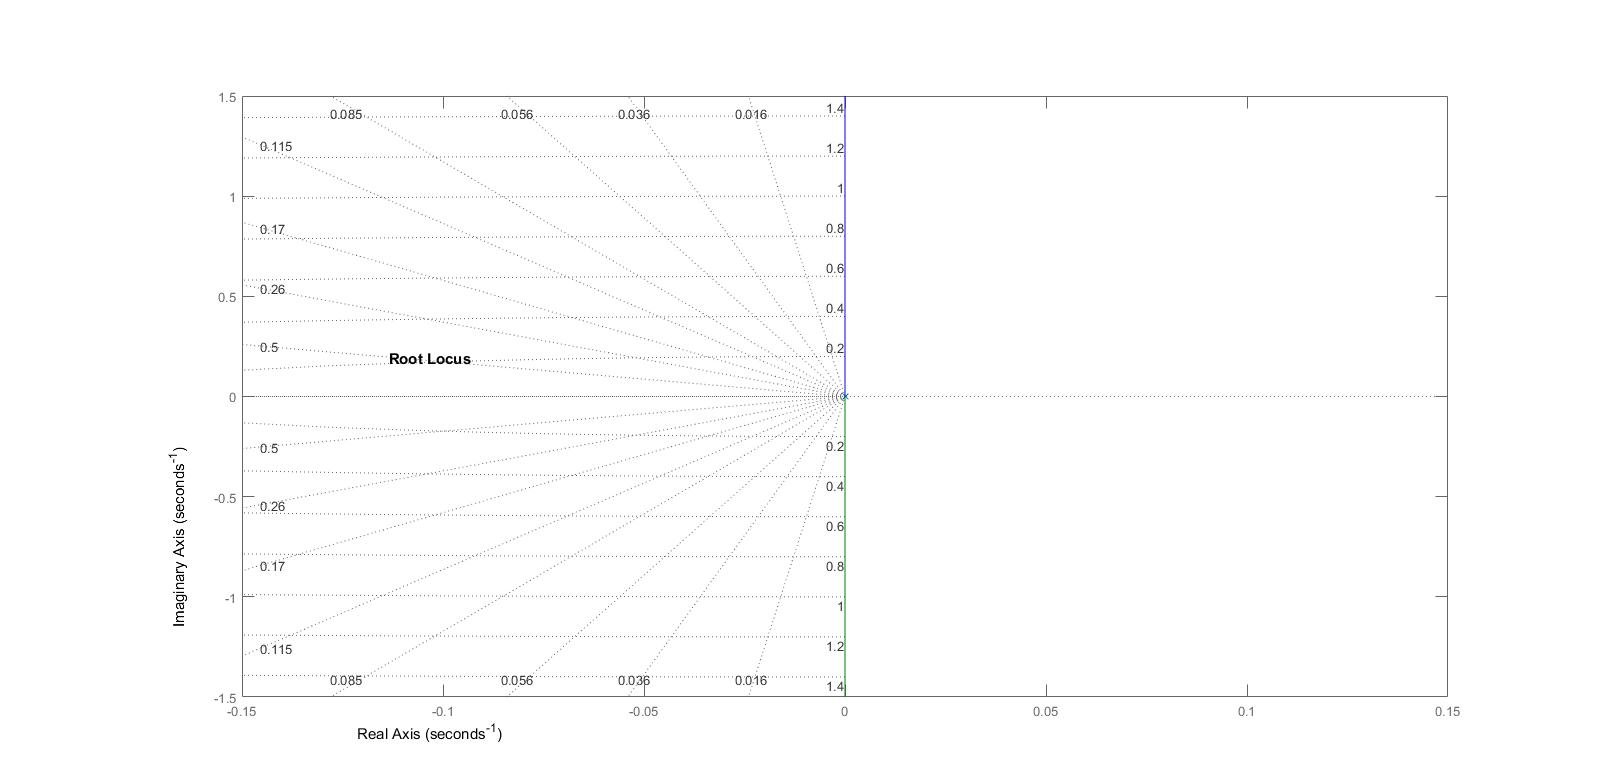
\includegraphics[width=\textwidth]{figures/Rocket/design/initial_transfer_function}
		\caption{Root locus of the initial rocket angle transfer function.}
		\label{fig:Rinitialtf}
	
\end{figure}

However the real system is influenced by the servomotors. The transfer function of the servomotors adds a pole, resulting in an unstable system moving towards infinity on the imaginary axis. 
				
				% Figure of tf + servo
\begin{figure}[htbp]
	\centering
		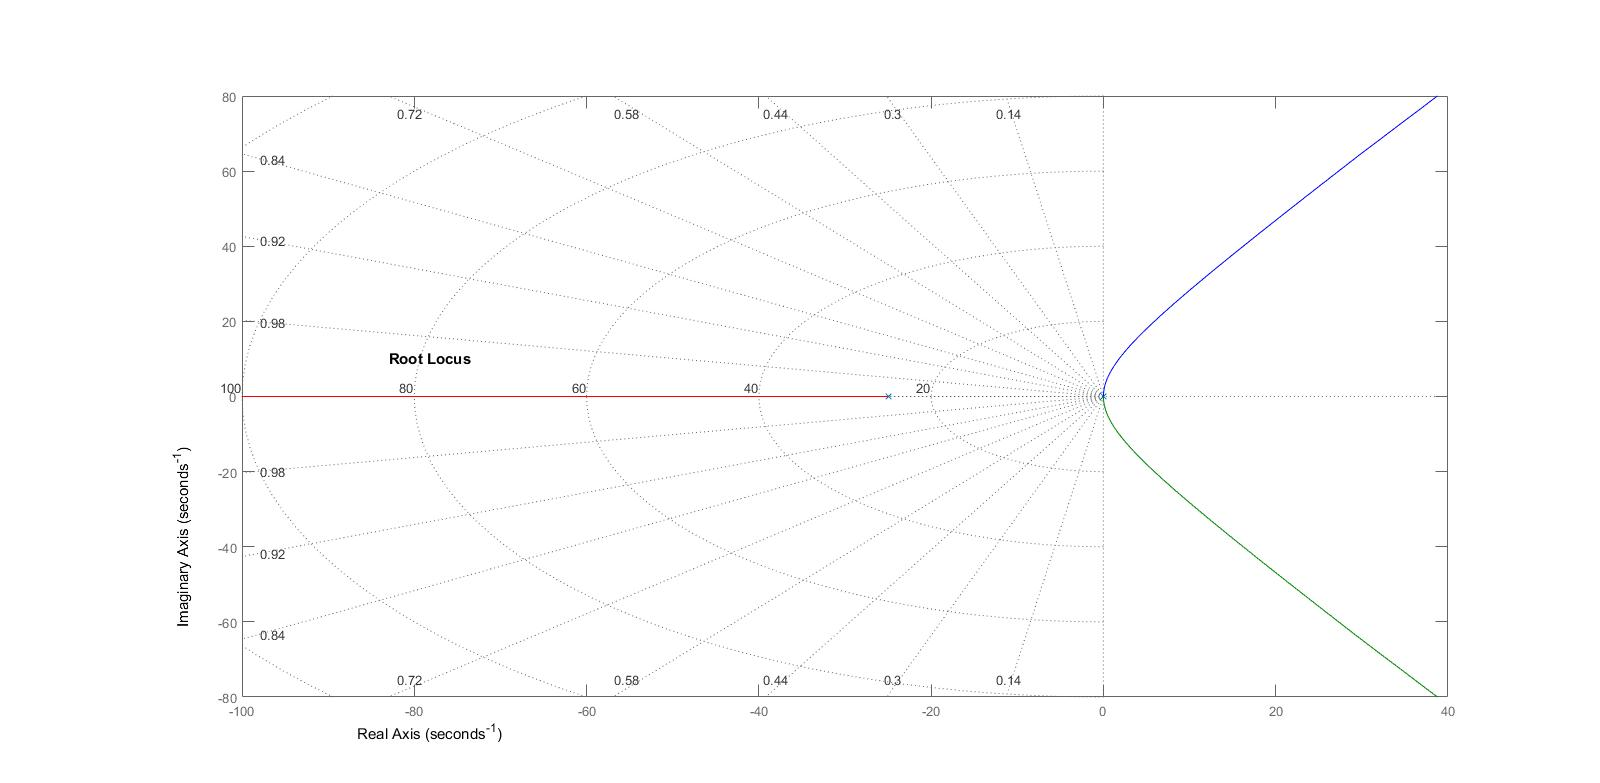
\includegraphics[width=\textwidth]{figures/Rocket/design/tf_with_servo}
		\caption{System with the servomotors.}
		\label{fig:SystemServo}
\end{figure}

To direct the root locus to a stable state, a controller C1, adding a zero and a pole on the left side, is implemented. The zero of the controller is chosen to be near the system in order to attract the poles. The pole of the controller is set at high frequency to not temper with the system. 

				% Figure of tf + servo + C1, and zoom of tf + servo + C1
\begin{figure}[htbp]
	\centering
	\begin{subfigure}{0.45\textwidth}
		\includegraphics[width=\textwidth]{figures/Rocket/design/tf_with_controller_1C_1}
		\caption{Total view of the poles and zeros.}
		\label{fig:SystemC1}
	\end{subfigure}
	\begin{subfigure}{0.45\textwidth}
		\centering
		\includegraphics[width=\textwidth]{figures/Rocket/design/tf_with_C1_zoom}
		\caption{Focus on low frequencies.}
		\label{fig:SystemC1zoom}
	\end{subfigure}
	\caption{Root locus of the system with C1 implemented.}
\end{figure}

Another controller C2 is needed to attract the two poles going to infinity along the imaginary axis. The pole and zeros of C2 are set at higher frequencies than the first controller C1. 

				% Figure of final tf with controllers 
\begin{figure}[htbp]
	\centering
	
		\includegraphics[width=\textwidth]{figures/Rocket/design/tf_with_controller_1}
		\caption{Root locus of the rocket transfer function.}
		\label{fig:SystemC1C2}
		
\end{figure}

The rocket requires a fast settling time and rise time in order to act as soon as possible and control the rocket's stability. Lead compensaters enable the modulation of the rise time, but impact the overshoot. The overshoot is considered as an inferrior error, being in part countered by the play of the gimbal system. 

To improve the setling time, the gain is set at $2.15 * 10^3$ \si{\dB}. This value is chosen by observing the root locus and the gain of a set point as shown on \autoref{fig:SystemC1C2Zoom}.

				% Figure of chosen point, and of final tf with 2.15*10^3
\begin{figure}[htbp]
	\centering
	\begin{subfigure}{0.45\textwidth}
		\includegraphics[width=\textwidth]{figures/Rocket/design/tf_with_controller_1_zoom}
		\caption{Set point at the start of the circle.}
		\label{fig:SystemC1C2Zoom}
	\end{subfigure}
	\begin{subfigure}{0.45\textwidth}
		\centering
		\includegraphics[width=\textwidth]{figures/Rocket/design/tf_with_controller_215}
		\caption{Additional gain of $2.15*10^3$ \si{\dB}.}
		\label{fig:SystemGain215}
	\end{subfigure}
	\caption{Root locus of the rocket transfer function with additional gain of respectively $1$ and $2.15*10^3$ \si{\dB}.}
\end{figure}


The servomotors can have a faster rising time according to the step response of the servomotors, as shown in \autoref{tab:TableStepr}. The gain is then doubled to improve the rise time and setling time. The new adjusted transfer function is observed on \autoref{fig:FinalRocketTf} and \autoref{fig:FinalRocketTfZoom}.

\begin{table}[htbp]
	\centering
	\caption{Simulated step responses.}
	\label{TableStepr}
	\begin{tabular}{llll}
		Transfer function & Rise time{(}s{)} & Setling time{(}s{)} & Overshoot{(}percentage{)} \\ \hline  \rowcolor{lightGrey}
		Servomotors     & 0.0589 & 0.0782 & 0\\  
		Gain of $2.15*10^3$     & 0.1669 & 1.2075 & 14.5609  \\  
		\rowcolor{lightGrey}           
		Gain of $5*10^3$     & 0.0854 & 0.7845 & 12.0162      \\     
	\end{tabular}
\end{table}

				% Figure of final tf with 5*10^3
\begin{figure}[htbp]
	\centering
	\begin{subfigure}{0.45\textwidth}
		\includegraphics[width=\textwidth]{figures/Rocket/design/tf_with_controller_5}
		\caption{Root locus of the rocket transfer function with an additional gain of $5 * 10^3$ \si{\dB}.}
		\label{fig:FinalRocketTf}
	\end{subfigure}
	\begin{subfigure}{0.45\textwidth}
		\includegraphics[width=\textwidth]{figures/Rocket/design/tf_with_controller_5_zoom}
		\caption{Focus on lower frequencies.}
		\label{fig:FinalRocketTfZoom}
	\end{subfigure}
	\caption{Root locus of the rocket transfer function with additional gain of $5*10^3$ \si{\dB}.}	
\end{figure}


The frequency correponds to a complete rotation of the servomotors. At low frequencies a delay is observed on \autoref{fig:BodeplotFinalTf}. However the system functions at low speed. This implies that the delay has a tempered effect on the system. Higher frequencies are not physicaly possible and do not need to be compensated.

				% Figure of final tf bodepoint
\begin{figure}[htbp]
	\centering
		\includegraphics[width=\textwidth]{figures/Rocket/design/bodeplot}
		\caption{Bodeplot of the rocket transfer function.}
		\label{fig:BodeplotFinalTf}
\end{figure}

The controlled rocket transfer function is shown on equation \autoref{eq:RocketTfEqu} and figure \autoref{fig:FinalChart}.

\begin{equation}    \label{RocketTfEqu}
R = 5 \cdot 10^3 \cdot \frac{s + 2}{s + 1000} \cdot \frac{s + 50}{s + 1100} \cdot \frac{1}{s \cdot \uptau + 1} \cdot \frac{F_t \cdot L_{Cg} \cdot \frac{1}{M_r \cdot L_{Es}^2}}{s^2}  
\end{equation}

\begin{figure}[htbp]
	\centering
	
	\includegraphics[width=\textwidth]{figures/Rocket/design/final_chart}
	\caption{Rocket transfer function.}
	\label{fig:FinalChart}
	
\end{figure}

\part{Implementation}\label{pt:Implementation} 
\chapter{Implementation}
This chapter includes the implementation of controllers and components. The chapter will be seperated into two section, a section for the inverted pendulum and another section for the rocket. An Arduino will be used as the platform to implement the hardware and software on.    

\section{Inverted Pendulum Implementation}
This section describes the hardware and software implementation of the controllers designed cf. section \ref{sec:IPController}. The goal is to determine if the designed controllers will balance the stick in the real world application. The section is separated into three different parts about sensors, hardware controller and software controller. The first part is to implement the feedback for the controllers which in the case is sensors. 

\subsection{Implementing Sensors}
The following section describes the implementation of the sensors with an Arduino Uno and the double inverted pendulum setup.   

\subsubsection*{Potentiometer}\label{section:PotmeterImplementation}
The system consist of multiple sensors, as decribed cf. section \ref{sec:IPDesc}, where two of these are potentiometers. The potentiometers is tested cf. appendix \ref{appendix:PotMeterTest}. The appendix concluded with a first order approximation of both potentiometers. During implementation it is realized that a slight calibration were needed because of the potentiometer had shifted place in the setup. The approximation for Pot$_{arm}$ is:

\begin{equation}
\theta_a\ =\ 63,11 \cdot V_{{Pot}_{arm}} - 117,0
\end{equation}
\startexplain
	\explain{$\text{V}_{{Pot}_{arm}}$ is the output voltage of the arms potentiometer}{V}
	\explain{$\theta_a$ is the angle of the arm}{$^\circ$}
\stopexplain

The approximation for Pot$_{stick}$ is:

\begin{equation}
\theta_s\ =\ 66,66 \cdot \text{VPot}_{stick} - 163,9
\end{equation}

\startexplain
	\explain{$\text{V}_{{Pot}_{stick}}$ is the output voltage of the stick potentiometer.}{V}
	\explain{$\theta_s$ is the angle of the stick, but where zero degrees is when the stick has a zero degree deviation from the arm}{$^\circ$}
\stopexplain

An example of implementing this is done trough a pseudo-code which converts the analogue value to radians. The linear approximations of the potentiometers is used.
\begin{lstlisting}
void loop() {
  // read the input on A0 and A1:
  int PotArm = analogRead(A0);
  int PotStick = analogRead(A1);

  double VPotarm = PotArm / 204.8; //Analog2Voltage
  double ThetaA = 66.66 * VPotarm - 170.46; // Voltage2Degree
  double ThetaARad = ThetaA * (31.415926 / 1800.0); //Degree2Radians
  double VPotstick = PotStick / 204.8;
  double ThetaS = 63.64 * VPotstick - 117.77;
  double ThetaSRad = ThetaS * (31.415926 / 1800.0);
}
\end{lstlisting}    

The sampling time of the sensors is an important aspect when ensuring stability of the control system. The sensor sampling can not be to slow because then the control loops will be slow and not update fast enough. Considering that the sensor is a potentiometer which does not have any active components, then the only limit is the Arduino. Arduino specifies that calling a analogRead() takes approximately 100 $\upmu$s which corresponds to a sampling frequency of 10 kHz. This is considered fast enough for the system and is therefore not a problem. 

\subsubsection*{Tachometer}
The tachometer and its precision has been tested in appendix \ref{appendix:RPMTest}. The test concluded that the internal tachometers precision is within the limit of what could implemented. The tachometer outputs a voltage which is close to linear with the number of revolutions per minute.

The test concluded with a transfer function for the tachometer, that gives the relation between the tachometer voltage and motor velocity:
\begin{equation}
\dfrac{\dfrac{1000\ \text{RPM}}{3.130\ \text{V}} \cdot 2 \cdot \pi}{60\ \text{s}}\ \cdot\ T_{Voltage}[\text{V}]\ =\ M_{Velocity}\ \text{[rad/s]}
\end{equation}


The function can not directly be implemented with the Arduino. The tachometer will generate a negative and positive voltage corresponding to the direction of the motor. Negative voltage can not be directly input to the Arduino without short circuiting it, and the positive voltage would be to high considering that the motor can go up to 8500 RPM. Interfacing is therefore needed between tachometer and Arduino.
This interfacing is done trough the ESCON motor controller included in the inverted pendulum setup. The two outputs of the tachometer is put in to the motor controller via two analogue inputs. The one acts as the positive connection and the other as the negative. How the motor controller is reacting to an input is configured trough the ESCON studio included. In the case it is set with the conversion ratio from voltage to RPM on 3,130 V/1000 RPM, which was determined by external calibration from another tachometer and implemented in the software.  The motor controller is set with a output that converts this RPM down between 1 and 4 V to the Arduino. Where 1 V is corresponding to -3000 RPM and 4 V corresponding to +3000 RPM. This gives the possibility to convert these values back to RPM in Arduino. How the motor controller converts the voltages is considered a black box. The wiring for the tachometer can be seen cf. figure \ref{fig:EsconWiring}. 


\subsection{Implementing ESCON Motor Controller}
The following sections describes the implementation of the hardware motor controller with the Arduino. The motor controller in the setup is a Maxon Escon 50/5.

The Maxon ESCON 50/5 is a PWM servo controller, that can be used to control DC and EC motors. The application is to amplify signals and control systems trough different control operations. It can also be used with a PWM input signal that can be outputted as an amplified and higher frequency PWM signal to a motor. The servo controller can be used in three different modes which can be configured trough the included Maxon ESCON studio. It can be configured in two modes for speed control with open and closed loops with feedback from sensors trough the board, and one mode for motor current control trough inputs from other modules such as an Arduino. In the setup the Escon controller is set to current control.


It is setup trough the ESCON studio with current control, and with a external controlled PWM signal. It then gives the possibility to input a PWM signal from the Arduino, which will be amplified so that 90\% duty cycle equals 11 A and 10\% equals -11 A. This means that 50\% will give 0 A.


The Arduino uses a 8-bit timer for PWM as standard so to get a better resolution the TimerOne library is implemented. TimerOne is a 16-bit hardware timer which can be downscaled to give the possibility to have a 10-bit resolution on the PWM signal. A better resolution gives a higher number of duty cycle values which makes the control more precise than with 8-bit. 


The configuration file for the ESCON studio is included in the attachment files under "/Attachment/Implementation/Motor Controller/Motor Controller Configuration File". It can be imported into the ESCON studio and loaded onto any 50/5 controller.

The main specifications of the ESCON is listed cf. table \ref{MaxonSpecifications}.

\begin{table}[htbp]
	\centering
	\begin{tabular}{llll}
	\hline
	Parameter & Value & Unit \\ \hline
	Supply voltage V$_{cc}$& 10-50 V & {[}V{]} \\
	Output voltage (max.) & 0,98 $\cdot$ V$_{cc}$& {[}kg{]} \\
	Nominal output current & 5 & {[}A{]} \\
	Maximum output current (<20 s) & 15 & {[}A{]}\\
	Current control PWM frequency & 53,6 & {[}kHz{]}
	\end{tabular}
\caption{Maxon Escon 50/5 specifications\citep{datasheet:maxon}.}
\label{MaxonSpecifications}
\end{table}

They wiring for the setup can be seen cf. figure \ref{fig:EsconWiring}.  

\begin{figure}[htbp]
\centering
\includegraphics[width=0.85\linewidth]{figures/MotorControllerSetup}
\caption{Wiring for the control setup.}
\label{fig:EsconWiring}
\end{figure}
\newpage
The control PWM signal from the Arduino is set with a frequency of 5 kHz because that it is the maximum input frequency the motor controller will accept. It is set to 5 kHz so that the PWM avoids interference with the sampling frequency for the system.
The input PWM signal is then amplified and made faster. The output PWM frequency of the motor controller is 53,6 kHz with a duty cycle from 10 - 90\% which can not be changed in the ESCON studio. It is considered that the switching frequency of the ESCON is close to optimal when considering that the PWM frequencies is within the limit of what its datasheet specifies.   The main concern of a switching frequency of 53,6 kHz on the motor would be heat dissipation. Therefore the minimum PWM frequency for the motor is calculated to see if the motor controllers PWM frequency fits the motor.

\subsubsection{Calculating Minimum PWM Frequency}
The only PWM frequency considered is the minimum switching frequency for the motor. This is done by considering the motor resistance and inductance versus the maximum amount of current ripple wanted on the motor. The values for the resistance and the inductance of the motor are calculated in appendix \ref{tab_appendix:KeSetUp}. The formula is seen cf. \ref{eq:PWMSwitch} [Palle Andersen, 2016].

\begin{equation}
f_{switch} \geq \frac{-1}{2\cdot ln(1-\frac{p}{100})}\cdot\frac{R_{m}}{L_{m}}
\label{eq:PWMSwitch}
\end{equation}
Where:\\
\begin{tabular}{m{8em} m{25em} m{8em}}
$p$& The maximum \% current ripple in the motor. & [1]\\
$\frac{R_{m}}{L_{m}}$& The inverse electrical time constant of the motor.& [Hz]\\
\\
\end{tabular}

Replacing with the numerical values of the resistance and the inductance and choosing a max ripple percentage of 5\%, the minimum switching frequency determined to be:
\begin{equation}
    f_{switch} \geq \frac{-1}{2 \cdot ln(1-\frac{5}{100})}\cdot\frac{0,82\ \Omega}{156\cdot10^-6 \ \cdot \text{H}} \approx \ 51,2 \text{kHz}
\end{equation}

The maximum ripple in the motor is determined by making the ripple the unknown factor P$_{ripple}$ and setting the PWM frequency to the implemented 53,6 kHz.  

\begin{equation}
    53,6 \text{kHz} = \frac{-1}{2 \cdot ln(1-\frac{P_{ripple}}{100})}\cdot\frac{0,82\ \Omega}{156\cdot10^-6 \ \cdot \text{H}}\ =\ P_{ripple}\ = 4,785\%  
\end{equation}
This gives that the maximum current ripple is 4,785\% if considering a PWM frequency on 53,6 kHz. A general rule is that the ripple should be less than 10\% of the current, so considering that is less than 5\% is good considering that the system is implemented with current control.


%https://playground.arduino.cc/Code/Timer1
 
\subsection{Implementing Controllers}
The implementing on the hardware has been described in the chapter, and therefore the implementation can proceed to the implementing the controllers on an Arduino. 

\subsection{Implementing Continuous Controller on Arduino}
As the Arduino is a microprocessor the continuous controller found in \autoref{sec:IPController} needs to be transformed into a discrete controller. This also means a sample time needs to be determined. The sample time needs to be faster than the settling time of the fastest subsystem i.e. the motor loop. The motor loop has a settling time of 0.0137 seconds. The sample time is selected to be 0.002 seconds as it's faster than the motor loop. This gives a sampling frequency of \autoref{eq:ArduinoFs}.
\begin{flalign}
F_s=500\text{ Hz}\label{eq:ArduinoFs}
\end{flalign}

With the sampling time determined the continuous controller needs to be transformed to a discrete controller. For the two P-controllers it's as simple as multiplying the sampled input with the gain to get the discrete output. For the outer loop controller it's not as simple and is done by using the Z-transform. There are a couple of different options for performing the Z-transform each with their own nuances but the differences won't be discussed and the bilinear transform will be used. For the bilinear transform $s$ in \autoref{eq:outerLeadController} will be substituted with \autoref{eq:s=z}.
\begin{flalign}
s=2F_s\frac{z-1}{z+1}\label{eq:s=z}
\end{flalign}

\autoref{eq:outerLeadController} then becomes \autoref{eq:DxBilinear}.
\begin{subequations}\label{eq:DxBilinear}
\begin{flalign}
&D_x=8.8\frac{2F_s\frac{z-1}{z+1}+4.29}{2F_s\frac{z-1}{z+1}+9.19} \\
&D_x=8.8\frac{2F_s(z-1)+4.29(z+1)}{2F_s(z-1)+9.19(z+1)} \\
&D_x=8.8\frac{(2F_s+4.29)z+4.29-2F_S}{(2F_s+9.19)z+9.19-2F_s} \\
&D_x=\frac{Y(z)}{X(z)}=8.8\frac{2F_s+4.29+(4.29-2F_S)z^-1}{2F_s+9.19+(9.19-2F_s)z^-1} \\
&Y(z)\left(2F_s+9.19+(9.19-2F_s)z^-1\right)=8.8X(z)\left(2F_s+4.29+(4.29-2F_S)z^-1\right) 
\end{flalign}
\end{subequations}

The Z-transformed controller can then be made discrete by substituting $aY(z)z^m$ with $ay[k+m]$ and similarly for $X(z)$. This is gives the discrete controller ready to be implemented in the Arduino in \autoref{eq:DxDiscrete}.
\begin{subequations}
\begin{flalign}
&(2F_s+9.19)y[k]+(9.19-2F_s)y[k-1]=8.8(2F_s+4.29)x[k]+8.8(4.29-2F_S)x[k-1] \\
&y[k]=8.8\frac{2F_s+4.29}{2F_s+9.19}x[k]+8.8\frac{4.29-2F_S}{2F_s+9.19}x[k-1]-\frac{9.19-2F_s}{2F_s+9.19}y[k-1] \label{eq:DxDiscrete}
\end{flalign}
\end{subequations}



\subsubsection{Controller Software}
This sections describes the software implemented on the Arduino. The structure and processes is represented with a flowchart cf. figure \ref{fig:Flowchart}. The software can be found in the attached materials under "Attachment/Implementation/Arduino Software/InvertedPendulumControlSoftware"  
\begin{figure}[htbp]
\centering
\includegraphics[width=1\linewidth]{figures/Flowchart.pdf}
\caption{Flowchart for the implemented software on Arduino.}
\label{fig:Flowchart}
\end{figure}
\newpage

\subsection{Implementation Evaluation}
This following sections describes the different problems that occurred with the hardware and software trough out the implementation. They will be explained to show the progress trough out the implementation.
\\
\subsubsection{Filtering Sensors}
During implementation of the Arm Loop it was found that a shaking occurred trough the motor, gear and out to the arm. From testing higher gains it was found that the shaking was amplified and became more unstable with the higher gains. Testing of the hardware and software was done to determine from where this shaking was sourced. To start with the sensors was checked for noise and floating. This was done to remove incorrect readings and unstable sensors. The sensors was read trough a oscilloscope and it was found that the ESCON motor controllers PWM frequency was represented in the sensor signal. This can occur from incorrect ground or wires not correctly isolated. This problem was solved by adding a capacitor to the sensors as seen cf. figure \ref{fig:EsconWiring}. The capacitor is connected from signal wires to ground to make a low pass filter. 1 $\upmu$F is chosen, one for each signal wire and considering that it is two 10 k$\Omega$ potentiometers it will give a varying cut of frequency. The cut-off frequency is calculated to:       

\begin{equation}
\frac{1}{2\cdot \pi \cdot 10000\ \Omega \cdot 1 \cdot 10^{-6}\  \text{F}}\ =\ 15,92\ \text{Hz}
\end{equation}

\begin{equation}
\frac{1}{2\cdot \pi \cdot 2,97\ \Omega \cdot 1 \cdot 10^{-6}\  \text{F}}\ =\ 53,6\ \text{Hz}
\end{equation}

Considering that the resistance changes we need to go under $\approx$ 2,97 $\Omega$ before the cut-off frequency exceeds the frequency of the noise, and that any resistance higher will dampen with more than -3 dB. It is noticeable that the resistance values of the potentiometers is in between both limits of resistances and the noise is therefore dampened. The conclusions of adding these filters removed high frequency noise that made the arm shake less. There was still a small-amplitude shaking around the setpoint when the arm was at a position and kept there. This could be down to bad range and bad optimisation of bits in the software. The software is made with scaling from analogue values down to radians, which means that reading the arm potentiometer and having a analogue value from 235 to 527 and converting it down to -0,785 to 0,785 radians will mean that that first two bits is not optimized, because they are static or close to. This gives that the 10-bit resolution of the PWM is not used optimally when two is static, but it is still better than having 8-bit with two static. This can be optimize by either changing the range of the potentiometers to that the radian range was optimized to cover from 0-1023 and have a better bit/radians resolution. This solution could be done by having a operational amplifier with a gain of 4 and a 5 V saturation. The potentiometer should then be turned to that -0,785 is at the 0 point for the potentiometer. It can also be solved by changing the model and with the conversion trough out the software. Meaning that the analogue value would not be converted which would give a better resolution for the PWM output. Equally they can be combined for the best resolution. It is chosen to only implement the resolution optimization if and only if the acceptance test show that the system does not fulfil the set requirements.

\subsubsection{PWM Frequency Problems}
The stick control loop was implemented. The simulations gave gains and results that could be implemented on the system. When implemented it was found that the arm did not control correctly when the stick moved. Repetitive test gave the conclusions that the speed of the arm was to slow. Higher gains was implemented but did not give the wanted result and the gains was set back to the simulated. A oscilloscope test was made on the Arduino PWM frequency by measuring the input frequency on the motor controller. The test showed that the frequency was 100 Hz and not 5 kHz as expected. The software was revised and determined that TimerOne was used as timer twice, one for controlling PWM frequency and one for controlling the sampling time with an interrupt. The interrupt was removed and changed to a wait so that the sampling time was kept constant. The PWM frequency was then measured to be 5 kHz and the arm then behaved as wanted with the simulated gains.    

\subsubsection{I2T Limitation}
Another problem observed where a run time limit on the control system. The system would slow down after around approximately a minut but it was easily observed trough the ESCON studio that a I2T limit was reached on the motor controller. An I2T limit is an algorithm that is described by the nominal current, the motor peak current in rms, and the motor peak current in seconds. It is used to secure the motor and driver from damage and over heating. The parameters for the algorithm was set trough the ESCON studio, with a nominal current on 5 A, a peak current on 11 A, and a thermal time constant on 200 seconds. When the limit is reached the motor current only goes to 5 A so the motor controller is shut off so that it cools down and can then be used again.  


\section{Rocket Implementation}

\subsection{Implementing Inertial Measurement Unit}

The system consists of an Inertial measurment Unit (IMU) GY - 80. This implies that multiple integreted sensors can be used, as seen in \autoref{sec:Rocket_sencor_choice}. The PCB created and used is seen in appendix \todo{appendix of PCB to do}. 
Mulitple physical and software constraints have to be taken into account when implementing the system.

The rise time and setling time of the sensors are an important feature when ensuring the stability of the rocket. It cannot be too slow, otherwise the system will react to late to any angle variation. The rise time and setling time of the servomotors and rocket transfer function are described in %\auto{tab:TableStepr}.
 The process of the servomotors is then considered fast enough for the system, not interfering with the angle control process.

The vibration of the rocket is a physical difficulty for the sensors as the measurements might be distorted. The placement and fixation must be carefully thought, as described in appendix \todo{appendix to do}.

Of all the sensors available, only the gyroscope will be used in this project. This is due to the conditions of the rocket launch : the rocket will be attached to the ground, and will therefore have no use of all the potential of the IMU GY -80.

\subsection*{Gyroscope}

The system includes a L3G4200D 3-axis gyroscope. The gyroscope is described in appendix \todo{appendix to do}. 

An example of implementing is done through a pseudo-code which converts in degree the output of the sensor in order to trace the rotation and mouvement of the system. The angle are then analyzed to measure the angle variation, and then enable the system to correct the variation.

\subsection{Test of simulated flight}

The system is connected to the servomotors. The goal is to simulate manually an angle variation of the rocket body and see the reaction of the system on the servomotors and the thruster. If the real thruster angle is equal to the desired one, then the controller is deemed acceptable and the system as fullfilling the requirements.

The expirement set up is described in appendix \todo{appendix to do}. An example of implementing is done through 
\todo{do the code/expirement to finish that part}.

\subsection{Test of attached-rocket flight}

The expirement set up is described in appendix . 

\part{Test \& conclusion}\label{pt:test_conclusion}
\graphicspath{{figures/AcceptanceTest/}}

\section{Inverted Pendulum Acceptance Tests}\label{sec:InvPendAccTest}

In this section the tests to check whether the controllers designed for the inverted pendulum fit the requirements or not. As said in \autoref{sec:TestDesc} the first acceptance test will not be documented as it is more an implementation requirement than a test.

\subsection{Acceptance Test 2.}

The goal of this test is to see if the inverted pendulum's stick and arm stay within the limits set in Requirement 2 and 3 described in \autoref{sec:InvPendReq}. \autoref{fig:AccTest2Arm} and \ref{fig:AccTest2Stick} plots the angles of the arm and the stick over a period of \SI{30}{\second} the maximum and the minimum angles are put in evidence so that it is easy to compare them with the requirements.

\begin{figure} [htbp]
	\centering
	\includegraphics[width=0.7\textwidth]{AngleArmplot}
	\caption{Plot of the angle of the arm over time with the limits set by the Requirement 1.}
	\label{fig:AccTest2Arm}
\end{figure}

From \autoref{fig:AccTest2Arm} it can be easily seen that the arm is within the requirements by a large margin of \SI{0.68}{\radian} or \SI{38.96}{\degree}. This result is due to the transformation of the outer loop described in \autoref{subsec:InvPendOuterLoopRedef}. Indeed the reference is not anymore the upright angle of the stick but the distance of a point on the stick compared with its position when both the arm and the stick are in upright position. Due to this the controller will try to keep both the arm and the stick in the upright angle which explains the very low angle variation of the arm compared to the requirement.

\begin{figure} [htbp]
	\centering
	\includegraphics[width=0.7\textwidth]{AngleStickplot}
	\caption{Plot of the angle of the Stick over time with the limits set by the Requirement 2.}
	\label{fig:AccTest2Stick}
\end{figure}

In \autoref{fig:AccTest2Stick} the largest angle the stick takes is \SI{0.05}{\radian} while the Requirement 2 precise a limit of \SI{0.9}{\radian}. So once again the requirement is respected by a large margin.

From the results seen it can be concluded that the second acceptance test is a success.

\subsection{Acceptance Test 3.}

Unfortunately a method to precisely hold and release the stick was not found, as such no precise data were able to be collected for this test. However, a video was taken during the test and will be joined with the report. This video shows the reactions of stick when different push are applied to it. The maximum angle for the arm and the stick are present and can be used as reference point. It can be noted that during the whole video the stick keeps its balance.

The results for the acceptance test of the stick are a success.
\chapter{Discussion}\label{sec:Discussion}

\section{Inverted Pendulum possible improvements}

The inverted pendulum as it is does fulfill all requirements. Furthermore, the possible simple improvements such as the suppression of the shaking is already discussed in \autoref{sec:InvPendImp}. So there is not much to talk about. What could have been done however, is to try other control design schemes such as space equations or bode plot and test them to see which one performs the best. Unfortunately too much time was wasted on fixing the set up to be able to do so.

\section{Rocket}



\section{Differences between the Rocket and the Inverted Pendulum}

As explained in \autoref{chap:ModelComp} the models are lightly
 % Include chapters

% For use if report is split up in parts
\bookmarksetup{startatroot}% Goto root of Table of Contents
\addtocontents{toc}{\bigskip}% Add space before next item in Table of Contents

% Appearance of the bibliography
\iflanguage{english}{%
\bibliographystyle{setup/plainnat_en}%
}{%
\bibliographystyle{setup/plainnat_dk}%
}



\bibliography{bib/conference,bib/datasheets,bib/mastersthesis,bib/newsarticles,bib/phdthesis,bib/sciencearticles,bib/standards,bib/techreports,bib/websites,bib/books}
\label{bib:mybiblio}



%\setlength{\chapnumb}{2cm} % Ændrer længden på stregen under kapiteloverskriften så den passer til bilag

\appendix % Start of appendix
\graphicspath{{figures/appendices/}}

%\include{chapters/appendices/PsocMasterCode}

\graphicspath{{figures/design/}}
\chapter{Test Journal: Template}
\begin{table}[!h]
\begin{tabular}{l l}
\textbf{Test participants:} & Maxime \& Robin \& Bang  \\
\textbf{Date:}  & 12/10-2016
\end{tabular}
\end{table}

\section*{Purpose}
The purpose of the test is to calculate the internal resistance and inductance for the DC motor.
\section*{Test equipment and components}
\begin{table}[h]
	\centering
	\caption{List of measurement equipment and components}\label{tab_appendix:template}

	\begin{tabularx}{\textwidth}{lXXXX}
		Name 				& Brand	& Model & AAU-number									\\ \toprule \rowcolor{lightGrey}
		Multimeter	& Fluke & 37 & 08181 	\\
		Powersupply	& Hameg triple & HM7042 & 33902\\ \rowcolor{lightGrey}
		DC motor & Maxon & 41.023.038-00.00-052& N/A
	\end{tabularx}
\end{table}
\section*{Setup}
Measurement setup is seen on \autoref{fig:DCSetup} \
\begin{figure} [h]
\centering
\includegraphics[width=0.6\linewidth]{figures/frontpage.jpg}
\caption{Measurement setup.}
\label{fig:DCSetup}
\end{figure}

Pictures and describing text
\section*{Method}
Step by step of test, maybe in enumerate
\begin{enumerate}
\item one
\item two
\end{enumerate}
\section*{Raw data}
Or maybe a plot if there's many results. (Remember to save the raw data anyway.)
\section*{Data processing}
\section*{Conclusion}



\graphicspath{{figures/appendix/"Motor&GearTests"/}}
\chapter{Test Journal: Gear Train System}\label{appendix:DCMotorInductance}
\begin{table}[htbp]
\begin{tabular}{l l}
\textbf{Test participants:} & Maxime \& Geoffroy  \\
\textbf{Date:}  & 28/2/2017
\end{tabular}
\end{table}

\section*{Purpose}
The objective of this test is to determine all the of the gear train system composed of the DC motor and the gear train.
\section{Electronics characteristics}

\subsection{Internal Resistance of the DC Motor $R_m$}
The first parameter to be tested is the internal resistance of the motor $R_m$. This resistance is needed in the motor's transfer function and will be used to determine the other parameters of the motor. 
\subsubsection*{Setup}
\autoref{fig:RmMeasurementSetup} shows a diagram and photo of the measurement set up
\begin{figure}[htbp]
	\centering
	\begin{subfigure}{0.50\textwidth}
		\includegraphics[width=1\textwidth]{figures/appendix/Motor&GearTests/RmTestSetUpDiagram}
		\caption{Diagram of the setup.} \label{fig:LaMeasurementDiagram}
	\end{subfigure}
	\begin{subfigure}{0.40\textwidth}
		\includegraphics[width=1\textwidth]{figures/figureIsComing}
		\caption{Picture of the setup.} \label{fig:LaMeasurementPictures}
	\end{subfigure}
	\caption{The measurement setup.} \label{fig:RmMeasurementSetup}   
\end{figure} 

\subsubsection*{Method}
This test consists of having the motor shaft locked while the voltage is increased by 0.5 V between measurements.

\subsubsection*{Raw data}
\autoref{tab_appendix:RmData} is the plotted evolution of the voltage of the circuit according to the current.

\begin{figure}[htbp]
	\centering
	\caption{Raw data used to determine $R_m$}\label{tab_appendix:RmData}
	\begin{tabularx}{0.35\textwidth}{XX}
		Voltage (V) & Current (A)\\ \toprule \rowcolor{lightGrey}
		0.50 & 0.33 \\
		1.00 & 0.71 \\ \rowcolor{lightGrey}
		1.50 & 1.13 \\
		2.00 & 1.67 \\ \rowcolor{lightGrey}
		2.49 & 2.34 \\
		2.98 & 2.94 \\ \rowcolor{lightGrey}
		3.50 & 3.75 \\
		3.99 & 4.68 \\ \rowcolor{lightGrey}
		4.50 & 5.54 \\
		4.98 & 6.11 \\ \rowcolor{lightGrey}
		5.54 & 6.46 \\
		6.02 & 7.40 \\ \rowcolor{lightGrey}
		6.51 & 8.26 \\
		7.01 & 9.14 
	\end{tabularx}
\end{figure}

\subsubsection{Data Processing}
In order to find the motor's resistance $R_m$, the electrical equations of the motor will be used:
\begin{equation}
	U_m = R_m \cdot i + L_m \frac{di}{dt} + K_e\omega_m
\end{equation}

With the motor shaft locked, $\omega_m = 0$. Moreover, the measurements are made a couple seconds after the change in voltage is made. The current is then constant, canceling its derivative. 

The resulting equation is Ohm's law:
\begin{equation}
U_m = R_m \cdot i
\end{equation}

The measurement of voltage according to the current is presented in \autoref{fig:Rmplot}.
\begin{figure}[htbp]
	\includegraphics[width=1\textwidth]{figures/modeling/Motor/Rmplot-converted-to-pdf}
	\caption{Diagram of the setup.} \label{fig:Rmplot}
\end{figure}

$R_m$ is the slope of the linear approximation (in dashed yellow) of the voltage over the current: 
\begin{subequations} \label{eq:LaEq}
	\begin{flalign}
		&U_m = R_m \cdot i \\
		&R_m \approx \SI{0.82}{\ohm}
	\end{flalign}
\end{subequations}


\subsection{Internal Inductance of the DC Motor $L_m$}
\begin{table}[htbp]
	\centering
	\caption{List of measurement equipment and components}\label{tab_appendix:LaSetUp}

	\begin{tabularx}{\textwidth}{lXXXX}
		Name 				& Brand	& Model & AAU-number									\\ \toprule \rowcolor{lightGrey}
		Oscilloscope	& Agilent & 54621D & 33941 	\\
		Powersupply	& Agilent & E3631A & 78577\\ \rowcolor{lightGrey}
		DC motor & Alsthom BBC & F9M2& 08339 
	\end{tabularx}
\end{table}
\subsubsection*{Setup}
\autoref{fig:LaMeasurementSetup} shows a diagram and photo of the measurement set up
\begin{figure}[htbp]
	\centering
	\begin{subfigure}{0.50\textwidth}
		\includegraphics[width=0.7\textwidth]{figures/appendix/Motor&GearTests/LmDiagram}
		\caption{Diagram of the setup.} \label{fig:LaMeasurementDiagram}
	\end{subfigure}
	\begin{subfigure}{0.40\textwidth}
		\includegraphics[width=1\textwidth]{MotorImpedanceTest.jpg}
		\caption{Picture of the setup.} \label{fig:LaMeasurementPictures}
	\end{subfigure}
	\caption{The measurement setup.} \label{fig:LaMeasurementSetup}   
\end{figure}

\subsubsection*{Method}
This test consists of having the motor shaft locked while a step is applied. The voltage of a shunt resistor is then measured by an oscilloscope from which the current is deduced.
\subsubsection*{Raw data}
\autoref{fig:LaTestCurrentPlot} is the plotted evolution of the current of the circuit in respect to time.

%\begin{figure}[htbp]
%	\centering
%	\includegraphics[width=0.7\textwidth]{LaTestCurrentPlot}
%	\caption{Plot of the current in respect to time}\label{fig:LaTestCurrentPlot}
%\end{figure}

\subsubsection*{Data processing}
When the shaft is locked and a step is applied the DC motor's electric equation can be resumed as in \autoref{eq:LaEquation}.
\begin{equation}
	F(s)=\frac{I_a(s)}{U_a(s)}=\frac{\frac{1}{R_a}}{\frac{L_a}{R_a} s+1} \addunit{1}
	\label{eq:LaEquation}
\end{equation}
\startexplain
\explain{$I_a(s)$ is the current in Laplace domain}{1}
\explain{$U_a(s)$ is the body's acceleration}{1}
\explain{$R_a$ is the internal resistance of the motor}{\si{\ohm}}
\explain{$L_a$ is the internal inductance of the motor}{\si{\henry}}
\stopexplain

When a unit step response is applied to the system \autoref{eq:LaEquation} becomes \autoref{eq:LaEquationStep}.

\begin{equation}
F(s)=\frac{\frac{1}{R_a}}{\frac{L_a}{R_a} s+1}\frac{1}{s}=\frac{-\frac{1}{R_a}}{s+\frac{R_a}{L_a}}+\frac{1}{R_a s} \addunit{1}
\label{eq:LaEquationStep}
\end{equation}

\autoref{eq:LaEquationStep} is then put in the continuous time domain to get \autoref{eq:LaEquationStepTime}.

\begin{equation}
f(t)= \frac{1}{R_a} \left(1-e^{-\frac{R_a}{L_a} t}\right) \addunit{1}
\label{eq:LaEquationStepTime}
\end{equation}

\autoref{eq:LaEquationStepTime} means that at $t=\frac{L_a}{R_a}$ the function would give $1-e^{-1}=\SI{63.212055882}{\percent}$ of its settling value. So at \SI{63.212055882}{\percent} of the settling value $t=\frac{L_a}{R_a}$ and since $R_a=\SI{0.43}{\ohm}$ \cite{datasheet:saradc} is known finding $L_a$ becomes trivial.

\subsubsection*{Conclusion}

Since the value of the current at the settling value is \SI{20.471}{\ampere}. Then \autoref{eq:LaEq} gives the value of $L_a$.

\begin{subequations} \label{eq:LaEq}
	\begin{flalign}
		&\frac{1}{R_a} \left(1-e^{-\frac{R_a}{L_a} \tau}\right)=20.471 \cdot 0.63212055882 \addunit{\second} \\
		&t = \SI{0.00190}{\second} \\
		&L_a=tR_a \\
		&L_a=\SI{817}{\micro\henry}
	\end{flalign}
\end{subequations}





\hrule

\hrule

\hrule

\hrule

\hrule

\hrule

SENSTOOL RmLm\\

\begin{table}[htbp]
	\centering
	\caption{List of measurement equipment and components}\label{tab_appendix:LaSetUp}
	
	\begin{tabularx}{\textwidth}{lXXXX}
		Name 				& Brand	& Model & AAU-number									\\ \toprule \rowcolor{lightGrey}
		
		DC motor & Alsthom BBC & F9M2 & 08339 
	\end{tabularx}
\end{table}


\subsubsection*{Setup}
\autoref{fig:KeMeasurementSetup} shows a diagram and photo of the measurement set up

\subsubsection*{Method}
The test will consist of applying a step of \SI{7}{\volt} on the DC motor (which is at \SI{0}{\volt} before that) with its shaft locked. Then via a curve fitting tool named SENSETOOL $R_m$ and $L_m$ are deduced.

\subsubsection*{Raw Data}
The blue line represents the power supply output without load.\\
The gold line is the response of the motor to this step.
\begin{figure}[htbp]
	\centering
	\includegraphics[width=\textwidth]{figures/appendix/Motor&GearTests/RmLmDataPlot}
	\caption{Plot of the voltage in respect to time of the input and the output of the DC motor}\label{fig:RmLmTestDataPlot}
\end{figure}

\subsubsection*{Data processing}

Since the shaft is locked, a step is applied and only the electrical characteristics of the motor are looked at. The data measured follows \autoref{eq:RmLmChar}.

\begin{equation} \label{eq:RmLmChar}
	u(t)=R_m i(t)+L_m \frac{d i(t)}{d t} \addunit{\volt}
\end{equation}

Which gives the transfer function \autoref{eq:RmLmTf}. Which is used to find $R_m$ and $L_m$ by curve fitting.

\begin{equation} \label{eq:RmLmTf}
\frac{I(s)}{U(s)}=\frac{1}{R_m +L_m s} \addunit{1}
\end{equation}

\subsubsection*{Conclusion}

After the curve fitting the following values are found $R_m=\SI{1.02}{\ohm}$ and $L_m=\SI{142}{\micro\henry}$. \autoref{fig:RmLmTestFitPlot} is a comparison between the model with these parameters and the measures done.

\begin{figure}[htbp]
	\centering
	\includegraphics[width=\textwidth]{figures/appendix/Motor&GearTests/RmLmFitPlot}
	\caption{Plot of the comparison between the model and the measures}\label{fig:RmLmTestFitPlot}
\end{figure}
\hrule

\hrule

\hrule

\hrule

\hrule

\hrule


\subsection{The DC Motor velocity constant $K_e$}
\begin{table}[htbp]
	\centering
	\caption{List of measurement equipment and components}\label{tab_appendix:KeSetUp}
	
	\begin{tabularx}{\textwidth}{lXXXX}
		Name 				& Brand	& Model & AAU-number									\\ \toprule \rowcolor{lightGrey}
		Oscilloscope	& Agilent & 54621D & 33941 	\\
		Powersupply	& Agilent & E3631A & 78577\\ \rowcolor{lightGrey}
		DC motor & Alsthom BBC & F9M2& 08339
	\end{tabularx}
\end{table}

\subsubsection*{Setup}
\autoref{fig:KeMeasurementSetup} shows a diagram and photo of the measurement set up
\begin{figure}[htbp]
	\centering
	\begin{subfigure}{0.50\textwidth}
		\includegraphics[width=\textwidth]{figures/appendix/Motor&GearTests/KeTestSetUp}
		\caption{Diagram of the set up.} \label{fig:KeMeasurementDiagram}
	\end{subfigure}
	\begin{subfigure}{0.40\textwidth}
		\includegraphics[width=1\textwidth]{figures/appendix/Motor&GearTests/KeTestPic}
		\caption{Picture of the set up.} \label{fig:KeMeasurementPictures}
	\end{subfigure}
	\caption{The measurement set up for $K_e$.} \label{fig:KeMeasurementSetup}   
\end{figure}

\subsubsection*{Method}
This test consists of having the motor shaft rotating in steady state while the voltage $U$ of the generator, the angular velocity $\omega$ of the shaft and the current $I$ are measured.

\subsubsection*{Raw data}
\autoref{tab_appendix:KeData} has all the measurements done.
\begin{figure}[htbp]
	\centering
	\caption{Raw data used to determine $K_e$}\label{tab_appendix:KeData}
	\begin{tabularx}{0.55\textwidth}{lXX}
		Voltage (V) & Current (A) & $\omega$ (rad/s)\\ \toprule \rowcolor{lightGrey}
		3.0  & 0.72 & 52.36  \\
		3.5  & 0.75 & 67.54  \\ \rowcolor{lightGrey}
		4.0  & 0.77 & 83.15  \\
		4.5  & 0.79 & 98.75  \\ \rowcolor{lightGrey}
		5.0  & 0.83 & 113.10 \\
		5.5  & 0.85 & 126.71 \\ \rowcolor{lightGrey}
		6.0  & 0.88 & 140.95 \\
		6.5  & 0.90 & 156.03 \\ \rowcolor{lightGrey}
		7.0  & 0.93 & 170.38 \\
		7.5  & 0.94 & 185.35 \\ \rowcolor{lightGrey}
		8.0  & 0.95 & 198.97 \\
		8.5  & 0.96 & 214.68 \\ \rowcolor{lightGrey}
		9.0  & 0.99 & 229.34 \\
		9.5  & 1.00 & 244.31 \\ \rowcolor{lightGrey}
		10.0 & 1.02 & 258.66 \\
		10.5 & 1.03 & 274.05 \\ \rowcolor{lightGrey}
		11.0 & 1.06 & 289.03 \\
		11.5 & 1.06 & 304.73 \\ \rowcolor{lightGrey}
		12.0 & 1.05 & 321.49
	\end{tabularx}
\end{figure}



\subsubsection*{Data processing}

When the shaft is rotating in steady state as shown in \autoref{fig:KeMeasurementDiagram}, \autoref{eq:KeSetUpElec} can be derived.
\begin{equation}
U=K_e\omega+R_m I \addunit{\volt}
\label{eq:KeSetUpElec}
\end{equation}

\startexplain
\explain{$I$ is the current in the circuit}{\si{\ampere}}
\explain{$U$ is the generator's voltage}{\si{\volt}}
\explain{$K_e$ is the velocity constant of the motor}{\si{\volt\per\radian\second}}
\explain{$R_m$ is the internal resistance of the motor}{\si{\ohm}}
\stopexplain

From \autoref{eq:KeSetUpElec} \autoref{eq:KeForm} is obtained by isolating $K_e$.

\begin{equation}
K_e=\frac{U-R_m I}{\omega} \addunit{\volt\per\radian\second}
\label{eq:KeForm}
\end{equation}

\subsubsection*{Conclusion}

\autoref{fig:KeTest} plot the $K_e$ found for each measurement. The $K_e$ used in the model is average of these points. This gives $K_e=\SI{0.0343}{\volt\per\radian\second}$

\begin{figure}[htbp]
	\centering
	\includegraphics[width=1.1\textwidth]{figures/appendix/Motor&GearTests/PlotKe}
	\caption{Plot of $K_e$ found for each measures}\label{fig:KeTest}
\end{figure}


\subsection{The DC Motor torque constant $K_t$}
\begin{table}[htbp]
	\centering
	\caption{List of measurement equipment and components}\label{tab_appendix:KtSetUp}
	
	\begin{tabularx}{\textwidth}{lXXXX}
		Name 				& Brand	& Model & AAU-number									\\ \toprule \rowcolor{lightGrey}
		Oscilloscope	& Agilent & 54621D & 33941 	\\
		Powersupply	& Agilent & E3631A & 78577\\ \rowcolor{lightGrey}
		DC motor & Alsthom BBC & F9M2& 08339
	\end{tabularx}
\end{table}

\subsubsection*{Setup}
\autoref{fig:KtMeasurementSetup} shows a diagram and photo of the measurement set up
\begin{figure}[htbp]
	\centering
	\begin{subfigure}{0.50\textwidth}
			\includegraphics[width=\textwidth]{KtTestSetUp}
		\caption{Diagram of the setup.} \label{fig:KtMeasurementDiagram}
	\end{subfigure}
	\begin{subfigure}{0.40\textwidth}
		%\includegraphics[width=1\textwidth]{MotorImpedanceTest.jpg}
		\missingfigure{Picture of the setup}
		\caption{Picture of the setup.} \label{fig:KtMeasurementPictures}
	\end{subfigure}
	\caption{The measurement setup.} \label{fig:KtMeasurementSetup}   
\end{figure}

\subsubsection*{Method}
This test consists of having the motor shaft locked while the torque $\tau_m$ and the current $I$ are measured.

\subsubsection*{Raw data}
\autoref{tab:KtTest} has all the measurements done.


\subsubsection*{Data processing}

When the motor is in steady state and the shaft locked as shown in \autoref{fig:KtMeasurementDiagram}, \autoref{eq:KtTest} is found from \autoref{eq:MotorTorque}.

\begin{equation}\label{eq:KtTest}
K_t=\frac{\tau_m}{I} \addunit{\newton\meter\per\ampere}
\end{equation}
\startexplain
\explain{$I$ is the current in the circuit}{\si{\ampere}}
\explain{$\tau_m$ is the torque of the motor}{\si{\newton\meter}}
\explain{$K_t$ is the motor's torque constant}{\si{\newton\meter\per\ampere}}
\stopexplain

\subsubsection*{Conclusion}

\autoref{fig:KtTest} plot the $K_t$ found for each measurement. The $K_t$ used in the model is average of these points. This gives $K_t=\SI{0.025}{\newton\meter\per\ampere}$

\begin{figure}[htbp]
	\centering
	\includegraphics[width=\textwidth]{figures/appendix/Motor&GearTests/RmLmDataPlot}
	\caption{Plot of $K_e$ found for each measures}\label{fig:KtTest}
\end{figure}

\section{Mechanical Characteristics}

\subsection{Frictions $B_m$}
\begin{table}[htbp]
	\centering
	\caption{List of measurement equipment and components}\label{tab_appendix:BmSetUp}
	
	\begin{tabularx}{\textwidth}{lXXXX}
		Name 				& Brand	& Model & AAU-number									\\ \toprule \rowcolor{lightGrey}
		Oscilloscope	& Agilent & 54621D & 33941 	\\
		Powersupply	& Agilent & E3631A & 78577\\ \rowcolor{lightGrey}
		DC motor & Alsthom BBC & F9M2& 08339
	\end{tabularx}
\end{table}

\subsubsection*{Setup}
\autoref{fig:BmMeasurementSetup} shows a diagram and photo of the measurement set up
\begin{figure}[htbp]
	\centering
	\begin{subfigure}{0.50\textwidth}
		\includegraphics[width=\textwidth]{BmTestSetUp}
		\caption{Diagram of the set up.} \label{fig:BmMeasurementDiagram}
	\end{subfigure}
	\begin{subfigure}{0.40\textwidth}
		%\includegraphics[width=1\textwidth]{MotorImpedanceTest.jpg}
		\missingfigure{Picture of the setup}
		\caption{Picture of the setup.} \label{fig:BmMeasurementPictures}
	\end{subfigure}
	\caption{The measurement set up.} \label{fig:BmMeasurementSetup}   
\end{figure}

\subsubsection*{Method}
This test consists of having the motor shaft running in steady state while the torque $\tau_m$, the shaft angular velocity $\omega$ and the current $I$ are measured.

\subsubsection*{Raw data}
\autoref{tab:KtTest} has all the measurements done.


\subsubsection*{Data processing}

The motor and the shaft are in steady state so $\tau_m=\tau_{fm}$ which combined with \autoref{eq:FrictionTorque} gives \autoref{eq:BmTest}.

\begin{equation}\label{eq:BmTest}
B_m=\frac{K_t I}{\omega} \addunit{\newton\per\radian\second}
\end{equation}
\startexplain
\explain{$I$ is the current in the circuit}{\si{\ampere}}
\explain{$K_t$ is the motor's torque constant}{\si{\newton\meter}}
\explain{$\omega$ is the shaft's angular velocity}{\si{\radian\per\second}}
\explain{$B_m$ is the viscous friction constant}{\si{\newton\per\radian\second}}
\stopexplain

\subsubsection*{Conclusion}

\autoref{fig:BmTest} plot the $B_m$ found for each measurement. The $B_m$ used in the model is average of these points. This gives $B_m=\SI{120}{\micro\newton\per\radian\second}$

\begin{figure}[htbp]
	\centering
	\includegraphics[width=\textwidth]{figures/appendix/Motor&GearTests/RmLmDataPlot}
	\caption{Plot of $B_m$ found for each measures}\label{fig:BmTest}
\end{figure}
\break

\subsection{Moment of Inertia of the Gears $J_gear$}

The moment of inertia of the gear train was thoroughly calculated in a previous report and will be used here.

\subsubsection*{Method}
The gear train can by divided in three parts: the large wheels, the small wheels and the axles. The latter is a solid cylinder whereas the wheels are considered as multiple hollowed cylinders. The moment of inertia about a symmetry axis through the center of mass for a hollow cylinder is described in \autoref{eq:MomentInertiaHollowedCylinder}: 
\begin{equation}
	J_{hc} = \frac{1}{2} M (R_1^2 + R_2^2)
	\label{eq:MomentInertiaHollowedCylinder}
\end{equation}
\startexplain
\explain{$J_{hc}$ is the moment of inertia about a symmetry axis through the center of mass for a hollow cylinder}{\si{\kilo\gram\meter\squared}}
\explain{$M$ is the mass of the hollowed cylinder}{\si{\kilo\gram}}
\explain{$R_1$ is the inner radius of the hollowed cylinder}{\si{\meter}}
\explain{$R_2$ is the outer radius of the hollowed cylinder}{\si{\meter}}
\stopexplain

For the axles, the inner radius $R_1$ is equal to zero, giving equation \autoref{eq:MomentInertiaSolidCylinder} for the solid cylinder.
\begin{equation}
	J_{sc} = \frac{1}{2} M R^2
	\label{eq:MomentInertiaSolidCylinder}
\end{equation}
\startexplain
\explain{$J_{sc}$ is the moment of inertia about a symmetry axis through the center of mass for a solid cylinder}{\si{\kilo\gram\meter\squared}}
\explain{$M$ is the mass of the solid cylinder}{\si{\kilo\gram}}
\explain{$R$ is the inner radius of the solid cylinder}{\si{\meter}}
\stopexplain

The mass of each wheels and axles are calculated using their volumes and the density of iron.

\begin{figure}[htbp]
    \centering
    \begin{minipage}[t]{0.45\textwidth}
        \centering
        \includegraphics[width=0.9\textwidth]{figures/appendix/Motor&GearTests/BigWheel} 
        \caption{Cross section of a large wheel \citep{web:BalancingStick2008}.}
    \end{minipage}\hfill
    \begin{minipage}[t]{0.45\textwidth}
        \centering
        \includegraphics[width=0.9\textwidth]{figures/appendix/Motor&GearTests/SmallWheel} 
        \caption{Cross section of a small wheel \citep{web:BalancingStick2008}.}
    \end{minipage}
\end{figure}

\subsubsection*{Conclusion}
The moment of inertia for each part of the gear system \citep{web:BalancingStick2008}:
\begin{subequations} \label{eq:ResumeMomentInertiaGears}
	\begin{flalign}
		\text{Large Wheel: } J_{Large} &= 1.433 \cdot 10^{-3} \ \si{\kilo\gram\meter\squared} \\
		\text{Small Wheel: } J_{Small} &= 0.037 \cdot 10^{-3}\ \si{\kilo\gram\meter\squared} \\
		\text{Axle 1: }\quad J_{A1} &= 0.083 \cdot 10^{-3}\ \si{\kilo\gram\meter\squared} \\
		\text{Axle 2: }\quad J_{A2} &= 0.078 \cdot 10^{-3}\ \si{\kilo\gram\meter\squared} \\
		\text{Axle 3: }\quad J_{A3} &= 0.092 \cdot 10^{-3}\ \si{\kilo\gram\meter\squared} 
	\end{flalign}
\end{subequations}

The total moment of inertia of the gear system can be calculated from \autoref{eq:TaufReorganized} in \autoref{sec:ModGearSys}.
\begin{equation}
	J_{gear} = N^2J_1 + N^4J_2 + N^6J_3
\end{equation}

With:
\begin{subequations} \label{eq:J1J2J3}
	\begin{flalign}
		J_{1} \:&=\: J_{Large} + J_{Small} + J_{A1} \:=\: 1.553 \cdot 10^{-3}\ \si{\kilo\gram\meter\squared} \\
		J_{2} \:&=\: J_{Large} + J_{Small} + J_{A2} \:=\: 1.548 \cdot 10^{-3}\ \si{\kilo\gram\meter\squared} \\
		J_{3} \:&=\: J_{Large} + J_{Small} + J_{A3} \:=\: 1.562 \cdot 10^{-3}\ \si{\kilo\gram\meter\squared} 
	\end{flalign}
\end{subequations}

Finally, $J_{gear}$ is calculated to be
\begin{equation}
	J_{gear} = 0.153 \cdot 10^{-3}\ \si{\kilo\gram\meter\squared}
\end{equation}




\chapter{Linearization of the Arm and Stick Model}
\label{sec:LinearStick}
This appendix will linearize \autoref{eq:unlinStick}
\begin{flalign}
J_s\ddot{\theta}_s = \frac{l_s}{2}M_s \Big( &-l_a\ddot{\theta}_a \cos(\theta_a-\theta_s)+l_a\dot{\theta}_a^2 \sin(\theta_a-\theta_s) \notag \\
&-\frac{l_s}{2}\ddot{\theta}_s -g\sin(\theta_s) \Big)-b_{as}\dot{\theta}_{as} \label{eq:unlinStick}
\end{flalign}
The linearization is made with a 1st order Taylor approximation. The linearization is done at the equilibrium point where the arm is in an upright position i.e. $\theta_s=0$. In the equilibrium point the derivatives of all the inputs and outputs are 0. In this case the inputs and outputs are $\theta_a$ and $\theta_s$ and the operating point is $\bar{\theta}_a=0$ and $\bar{\theta}_s=0$. The nonlinear model is expressed as a function of the inputs and outputs as seen in \autoref{eq:nonlinearmodel}.
\begin{flalign}\label{eq:nonlinearmodel}
f\left(\theta_a, \dot{\theta}_a, \ddot{\theta}_a, \theta_s, \ddot{\theta}_s\right)=\frac{l_s}{2}M_s \Big( &-l_a\ddot{\theta}_a \cos(\theta_a-\theta_s)+l_a\dot{\theta}_a^2 \sin(\theta_a-\theta_s) \notag \\
&-\frac{l_s}{2}\ddot{\theta}_s -g\sin(\theta_s) \Big)-b_{as}\dot{\theta}_{as}-J_s\ddot{\theta}_s
\end{flalign}

Generally all equilibriums can be found by setting \autoref{eq:nonlinearmodel} equal to 0 and the derivatives to 0 and solving for $\theta_a=\bar{\theta}_a$ and $\theta_s=\bar{\theta}_s$. For the pendulum it is easy to see the only two equilibriums are the stick pointing straight up and straight down. 

The 1st order Taylor approximation of an equation with multiple variables is seen in \autoref{eq:1stTaylor}.
\begin{flalign}
 f\left(\theta_a, \dot{\theta}_a, \ddot{\theta}_a, \theta_s, \ddot{\theta}_s\right) & \approx f\left(\bar{\theta}_a, 0, 0, \bar{\theta}_s, 0\right) + \left. \frac{\partial f}{\partial \theta_a}\right|_{(\bar{\theta}_a, \bar{\theta}_s)} \hat{\theta}_a \notag \\
& \phantom{=} + \left. \frac{\partial f}{\partial \dot{\theta}_a}\right|_{(\bar{\theta}_a, \bar{\theta}_s)} \hat{\dot{\theta}}_a + \left. \frac{\partial f}{\partial \ddot{\theta}_a}\right|_{(\bar{\theta}_a, \bar{\theta}_s)} \hat{\ddot{\theta}}_a \notag \\
& \phantom{=} + \left. \frac{\partial f}{\partial \theta_s}\right|_{(\bar{\theta}_a, \bar{\theta}_s)} \hat{\theta}_s + \left. \frac{\partial f}{\partial \ddot{\theta}_s}\right|_{(\bar{\theta}_a, \bar{\theta}_s)} \hat{\ddot{\theta}}_s \label{eq:1stTaylor}
\end{flalign}
\startexplain
	\explain{$\bar{\theta}$ denotes the angle in an operating point}{\si{\radian}}
	\explain{$\hat{\theta}$ denotes the angle of the small signal variances}{\si{\radian}}
\stopexplain

The three terms with sin or cos in \autoref{eq:JsShort} will be approximated individually using \autoref{eq:1stTaylor}, remembering that $\bar{\theta}=\bar{\dot{\theta}}=\bar{\ddot{\theta}}=0$ in the equilibrium.
\begin{subequations}
\begin{flalign}
 -l_a\ddot{\theta}_a\cos\left(\theta_a-\theta_s\right)  \approx & \ 0 + l_a\bar{\ddot{\theta}}_a\sin\left(\bar{\theta}_a-\bar{\theta}_s\right)\hat{\theta}_a  \notag \\ 
& -l_a\cos\left(\bar{\theta}_a-\bar{\theta}_s\right)\hat{\ddot{\theta}}_a - l_a\bar{\ddot{\theta}}_a\sin\left(\bar{\theta}_a-\bar{\theta}_s\right)\hat{\theta}_s   \\
 -l_a\ddot{\theta}_a\cos\left(\theta_a-\theta_s\right) \approx &-l_a\hat{\ddot{\theta}}_a 
\end{flalign} %\bar{\ddot{\theta}}_s
\end{subequations}
\begin{subequations}
\begin{flalign}
l_a\dot{\theta}_a^2\sin\left(\theta_a-\theta_s\right)  \approx &\ 0 + l_a\bar{\dot{\theta}}_a^2\cos\left(\bar{\theta}_a-\bar{\theta}_s\right)\hat{\theta}_a  \notag \\
& + 2l_a\bar{\dot{\theta}}_a\sin\left(\bar{\theta}_a-\bar{\theta}_s\right)\hat{\dot{\theta}}_a-l_a\bar{\dot{\theta}}_a^2\cos\left(\bar{\theta}_a-\bar{\theta}_s\right)\hat{\theta}_s   \\
 l_a\dot{\theta}_a^2\sin\left(\bar{\theta}_a-\bar{\theta}_s\right) \approx & \ 0 
\end{flalign}
\end{subequations}
\begin{subequations}
\begin{flalign}
& g\sin\left(\theta_s\right) \approx g\sin\left(\bar{\theta}_s\right) +g\cos\left(\bar{\theta}_s\right)\hat{\theta}_s \\
& g\sin\left(\theta_s\right) \approx g\hat{\theta}_s 
\end{flalign}
\end{subequations}

The linearized model then becomes \autoref{eq:LinearStick}.
\begin{flalign}
& J_s\hat{\ddot{\theta}}_s=\frac{l_s}{2}M_s\left(-l_a\hat{\ddot{\theta}}_a-\frac{l_s}{2}\hat{\ddot{\theta}}_s-g\hat{\theta}_s\right)-b_{as}\hat{\dot{\theta}}_{as} \label{eq:LinearStick}
\end{flalign}
 % Include appendices

\end{document}
